\chapter{Heatmaps for DGE} \label{de-heatmaps}
%\section{Heatmaps for PCx-PD comparisons} 

\begin{figure}[!ht]
    \centerline{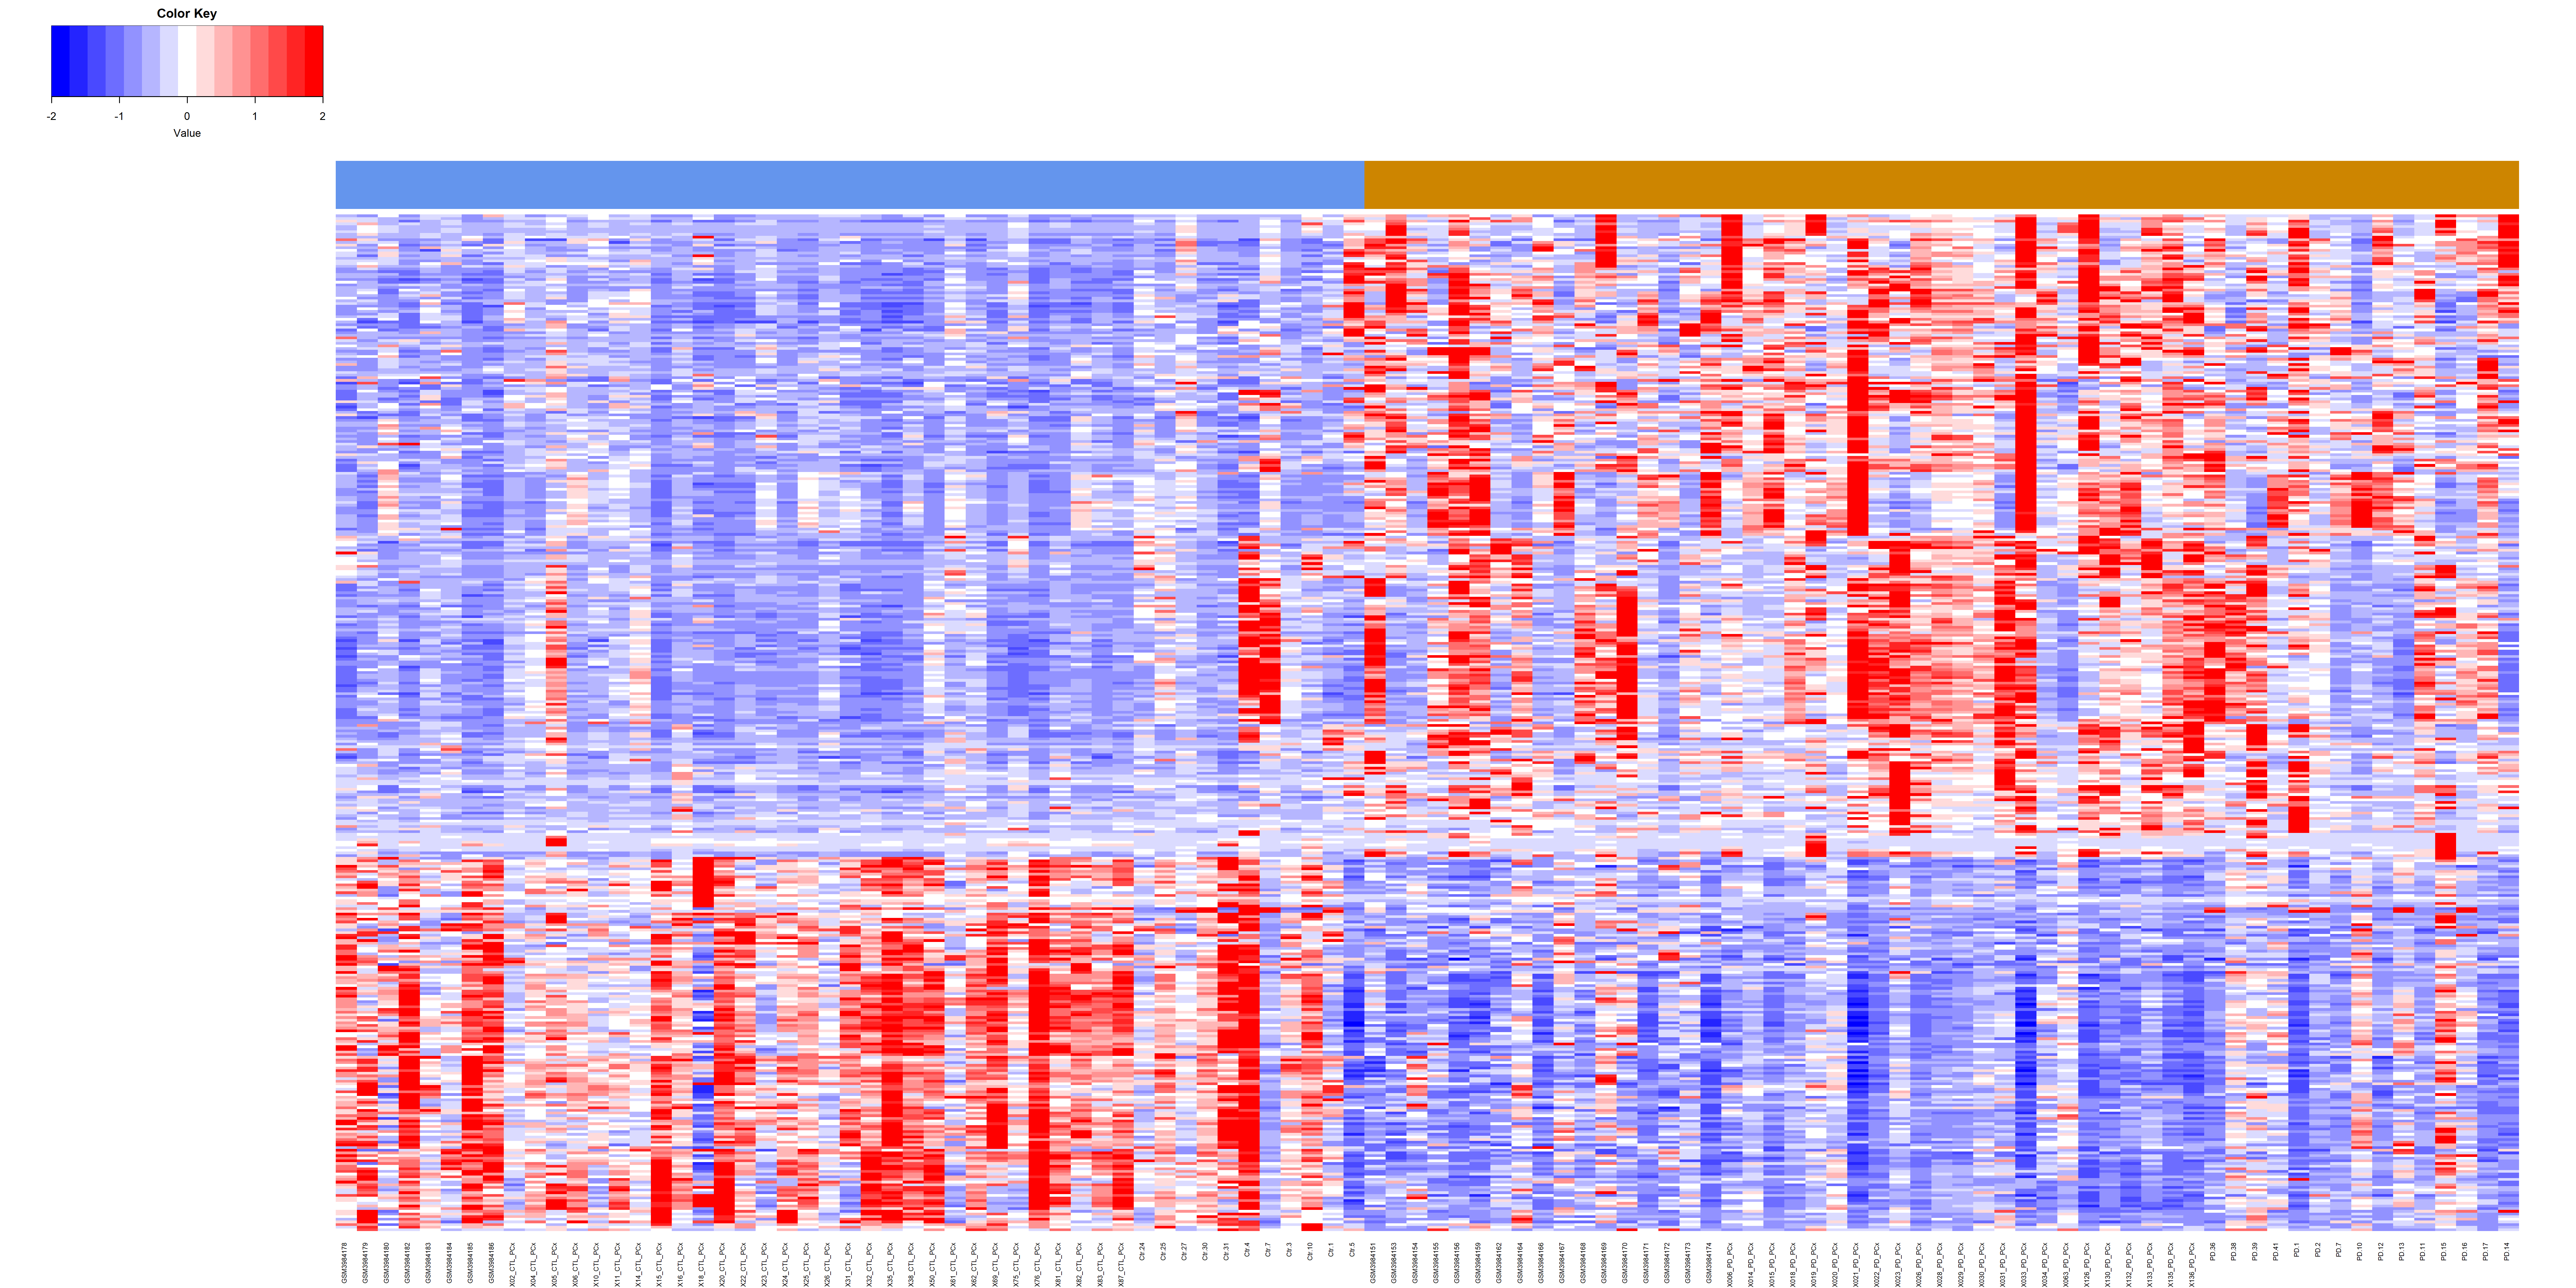
\includegraphics[width = 11cm]{Figures/DE heatmap/CTLvsPD-PCx_all.png}}
\caption{Heatmap of PCx-PD dataset for all the differentially expressed genes.}
\label{DE-pcx-pd}
\footnotesize $|$LFC$| >$ 1; PD is the contrast reference. Blue bar: control samples; golden bar: PD samples.
\end{figure}

\begin{figure}[!ht]
    \centerline{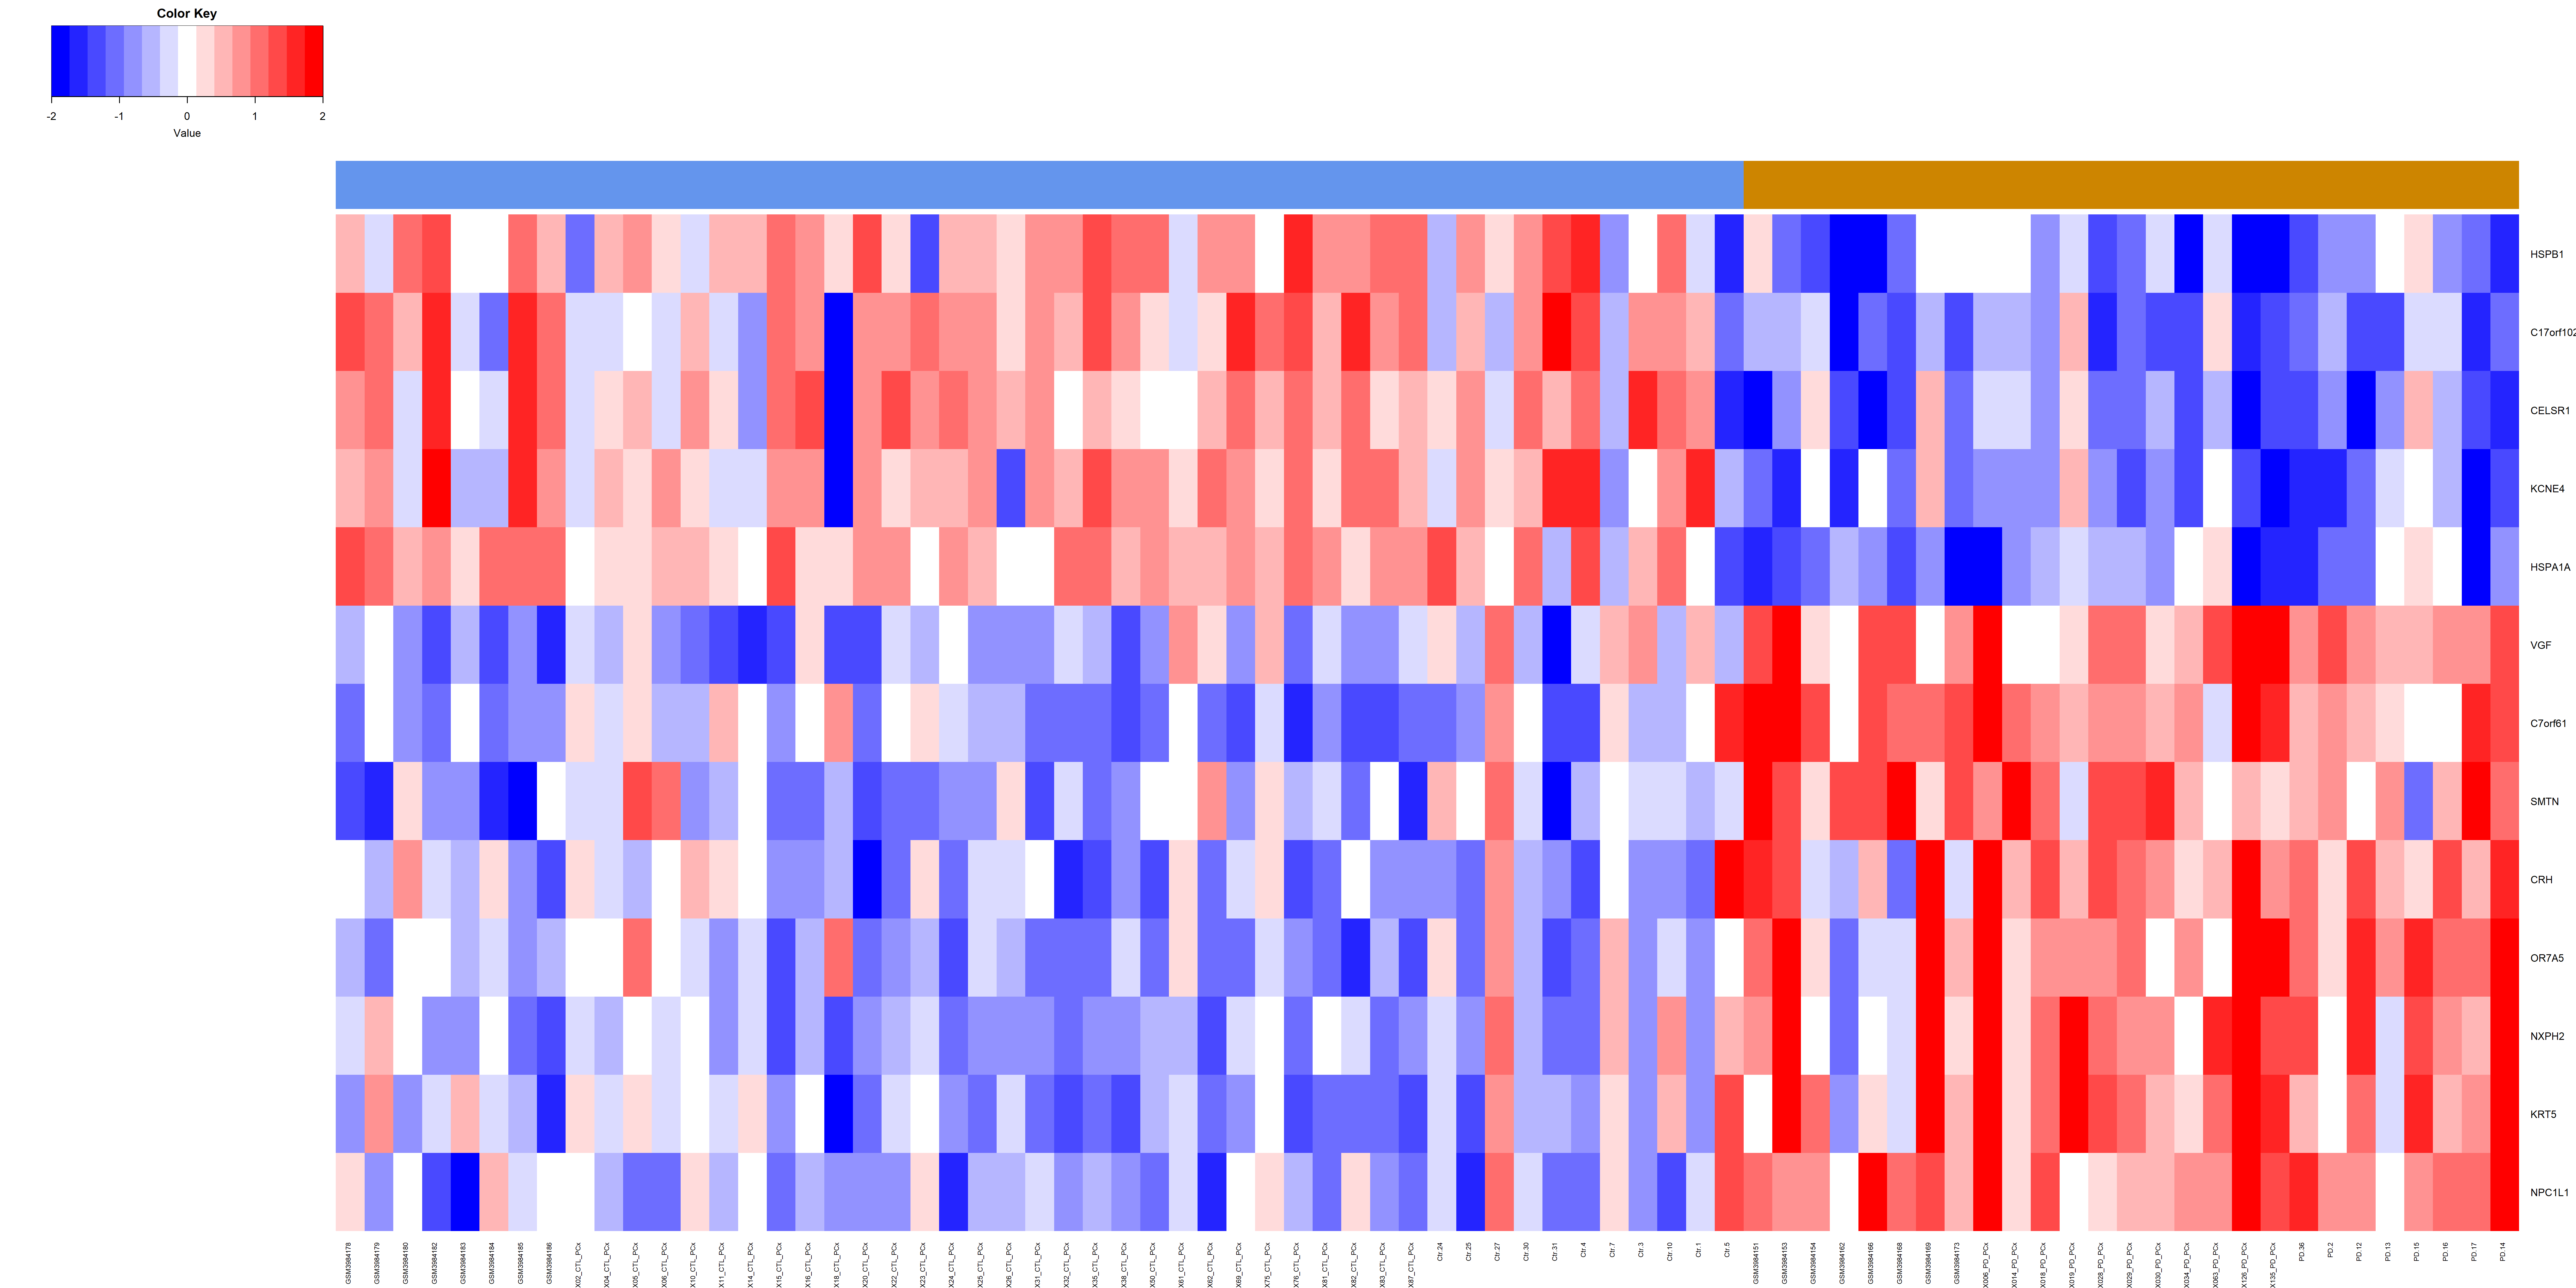
\includegraphics[width = 11cm]{Figures/DE heatmap/CTLvs1_PD-PCx.png}}
\caption{Heatmap of PCx-PD dataset for all the differentially expressed genes between control and subtype 1.}
\footnotesize $|$LFC$| >$ 1.6; case is the contrast reference. Blue bar: control samples; golden bar: S1 samples.
\end{figure}

\begin{figure}[!ht]
    \centerline{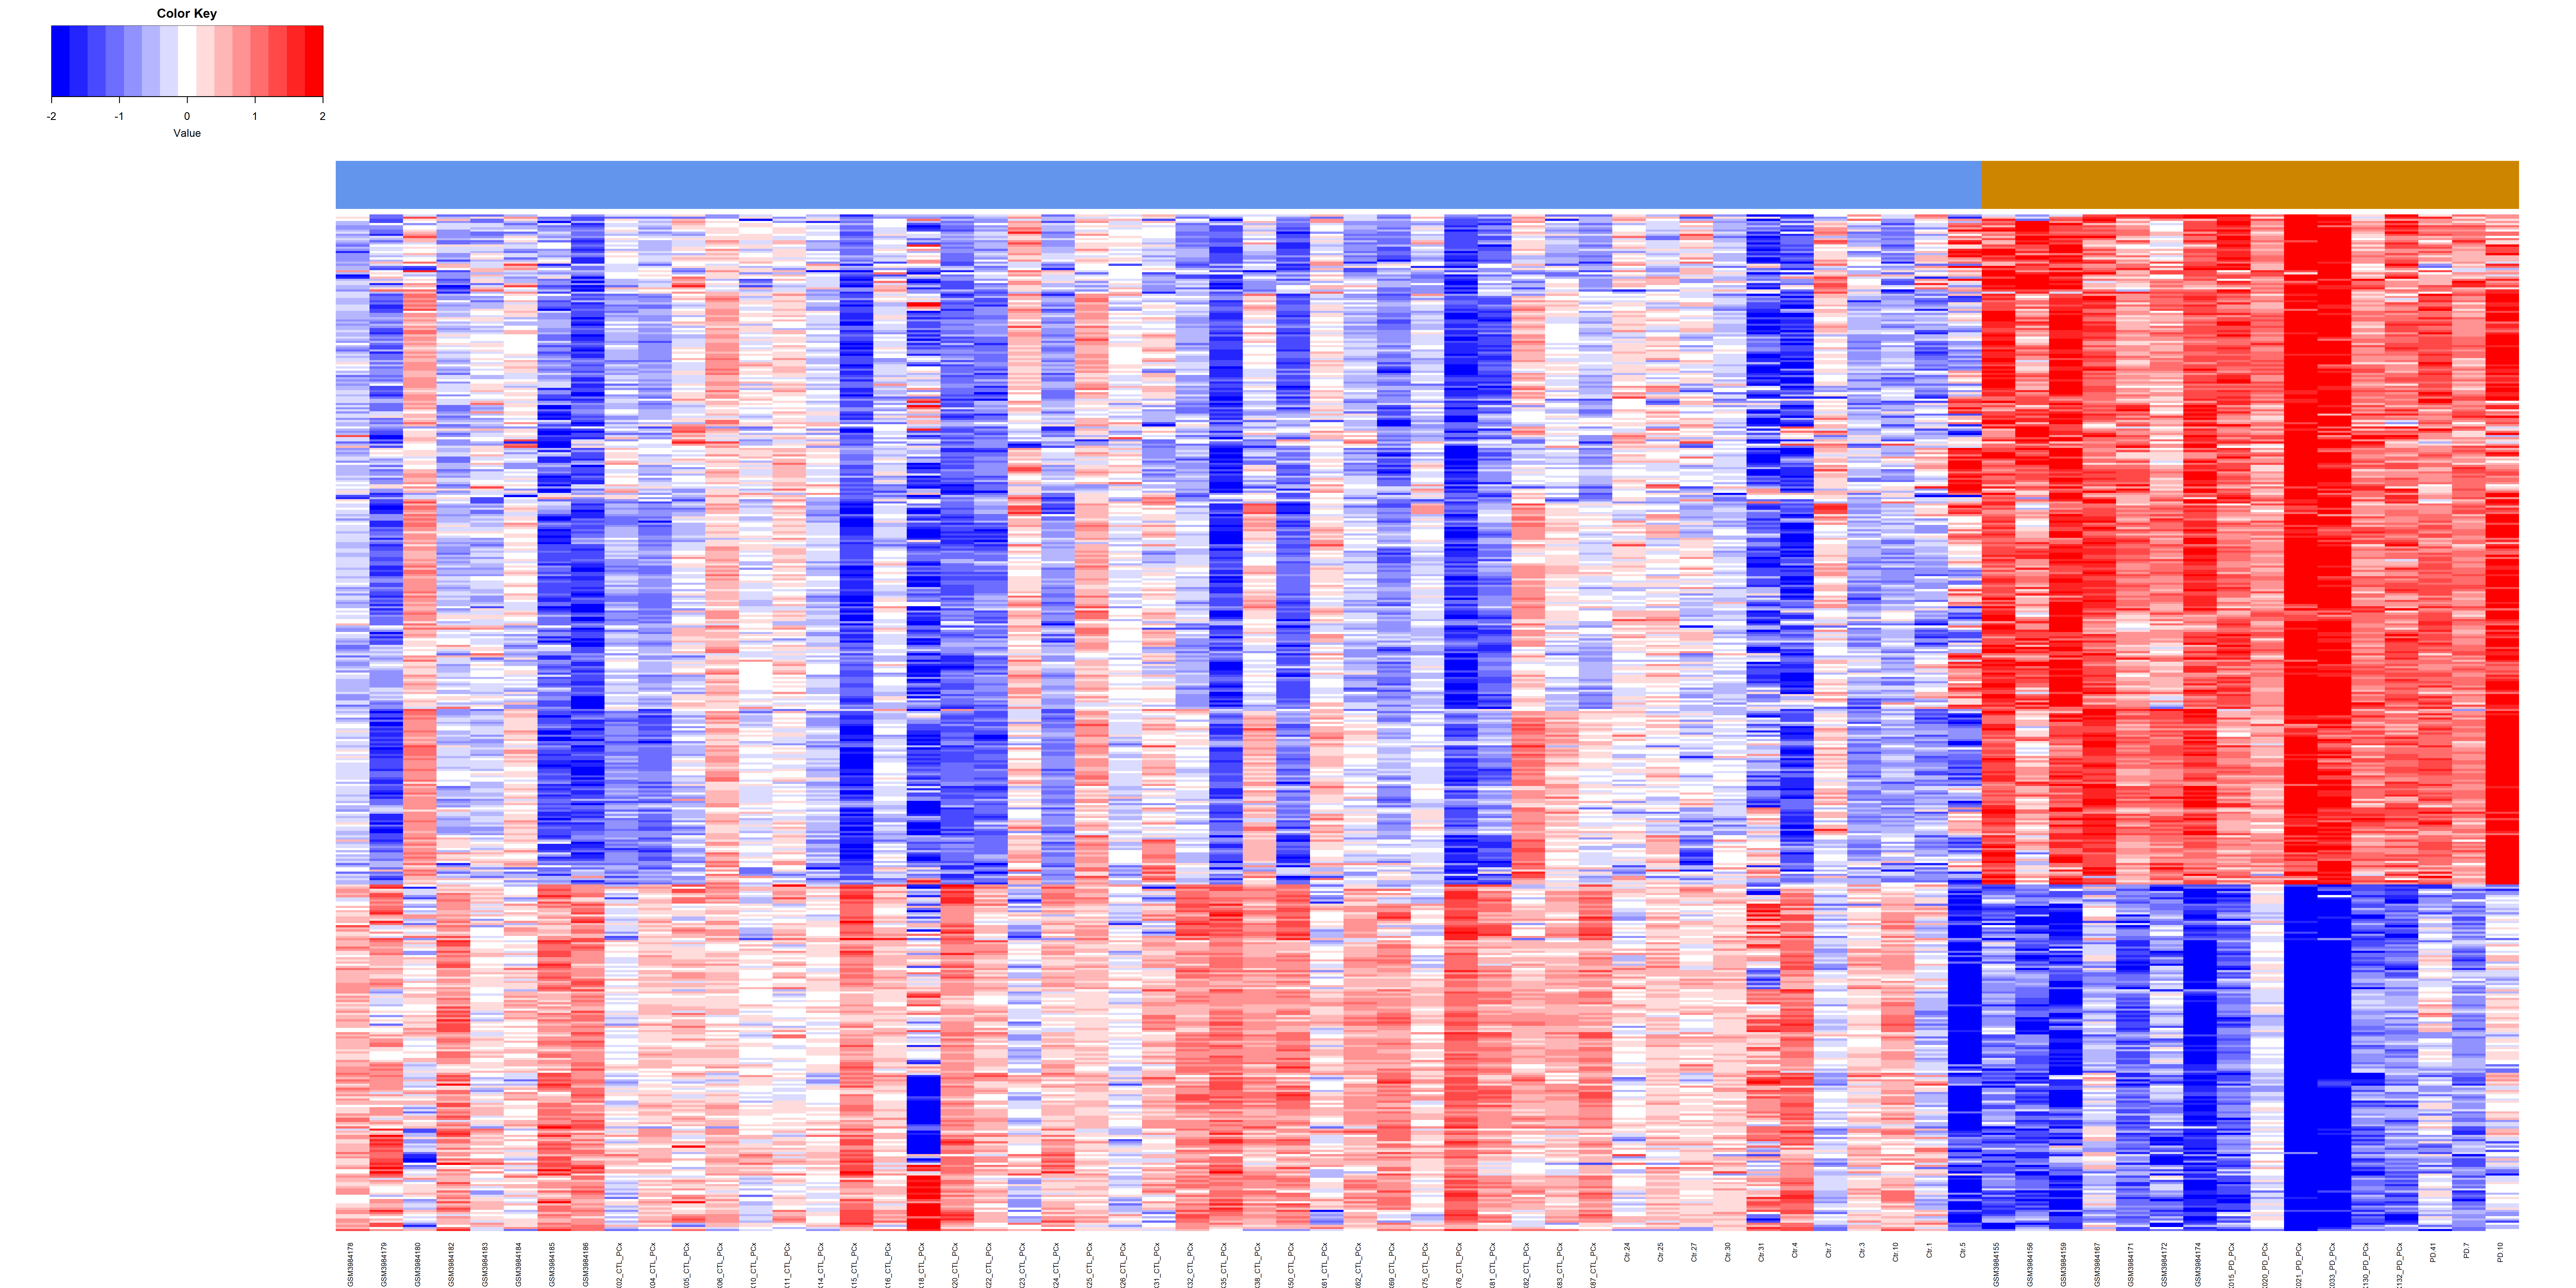
\includegraphics[width = 11cm]{Figures/DE heatmap/CTLvs2_PD-PCx_all.png}}
\caption{Heatmap of PCx-PD dataset for all the differentially expressed genes between control and subtype 2.}
\footnotesize $|$LFC$| >$ 1.6; case is the contrast reference. Blue bar: control samples; golden bar: S2 samples.
\end{figure}

\begin{figure}[!ht]
    \centerline{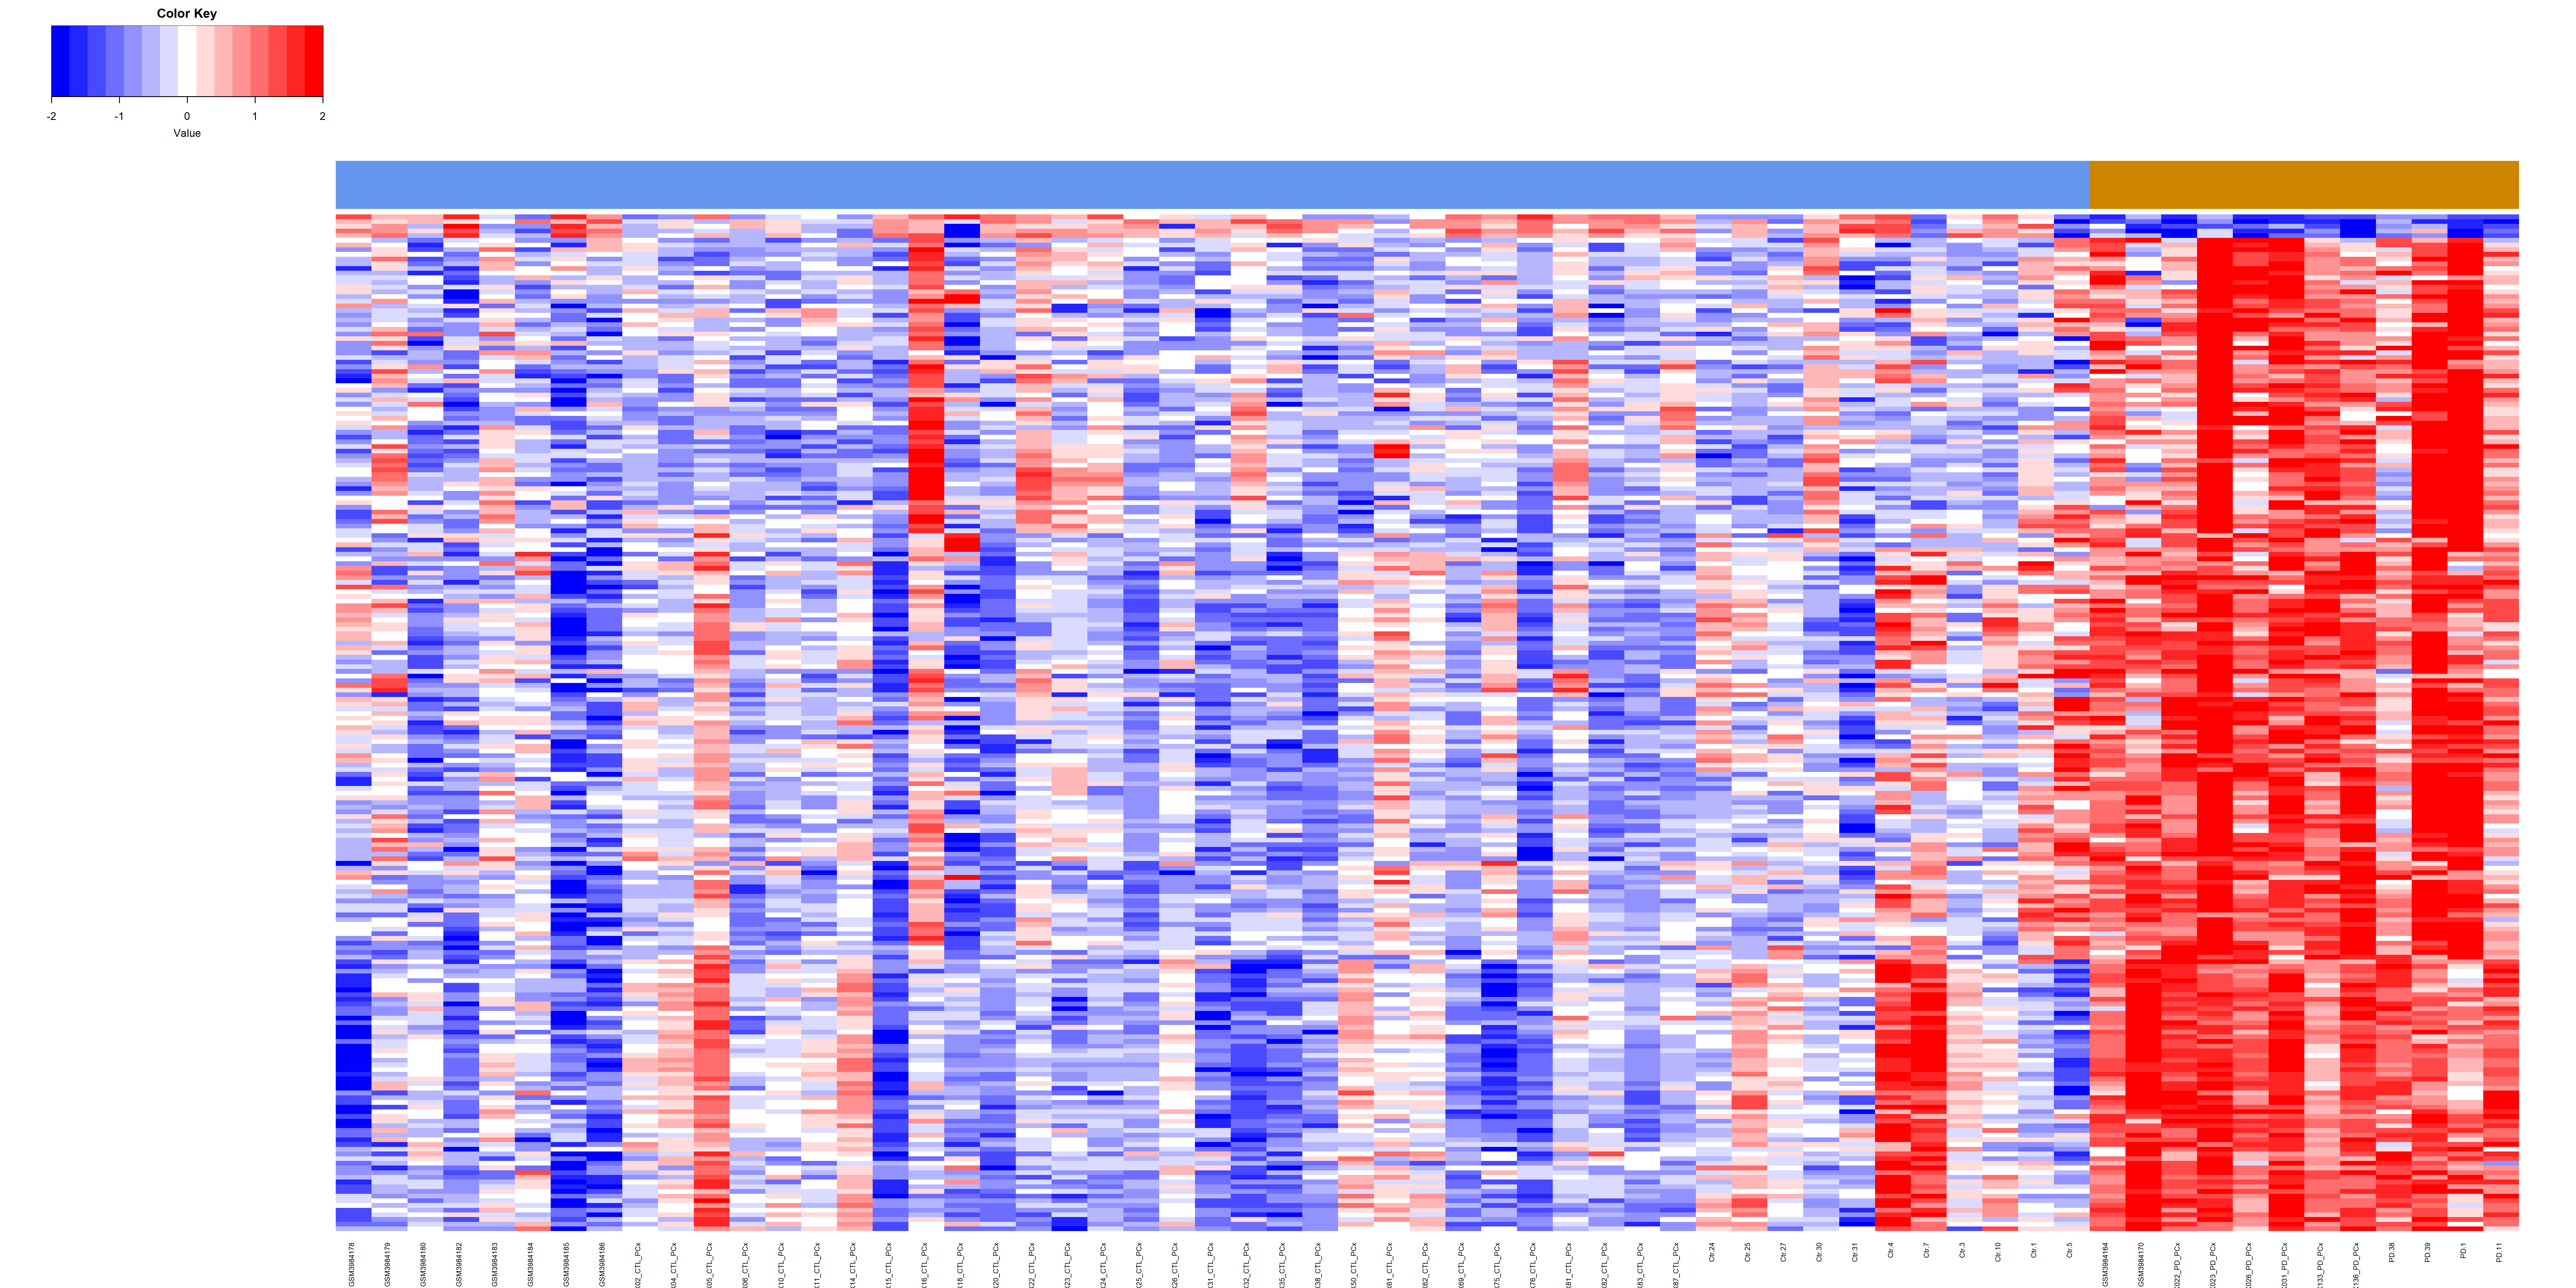
\includegraphics[width = 11cm]{Figures/DE heatmap/CTLvs3_PD-PCx_all.png}}
\caption{Heatmap of PCx-PD dataset for all the differentially expressed genes between control and subtype 3.}
\footnotesize $|$LFC$| >$ 1.6; case is the contrast reference. Blue bar: control samples; golden bar: S3 samples.
\end{figure}

%\section{Heatmaps for PCx-HD comparisons} 

\begin{figure}[!ht]
    \centerline{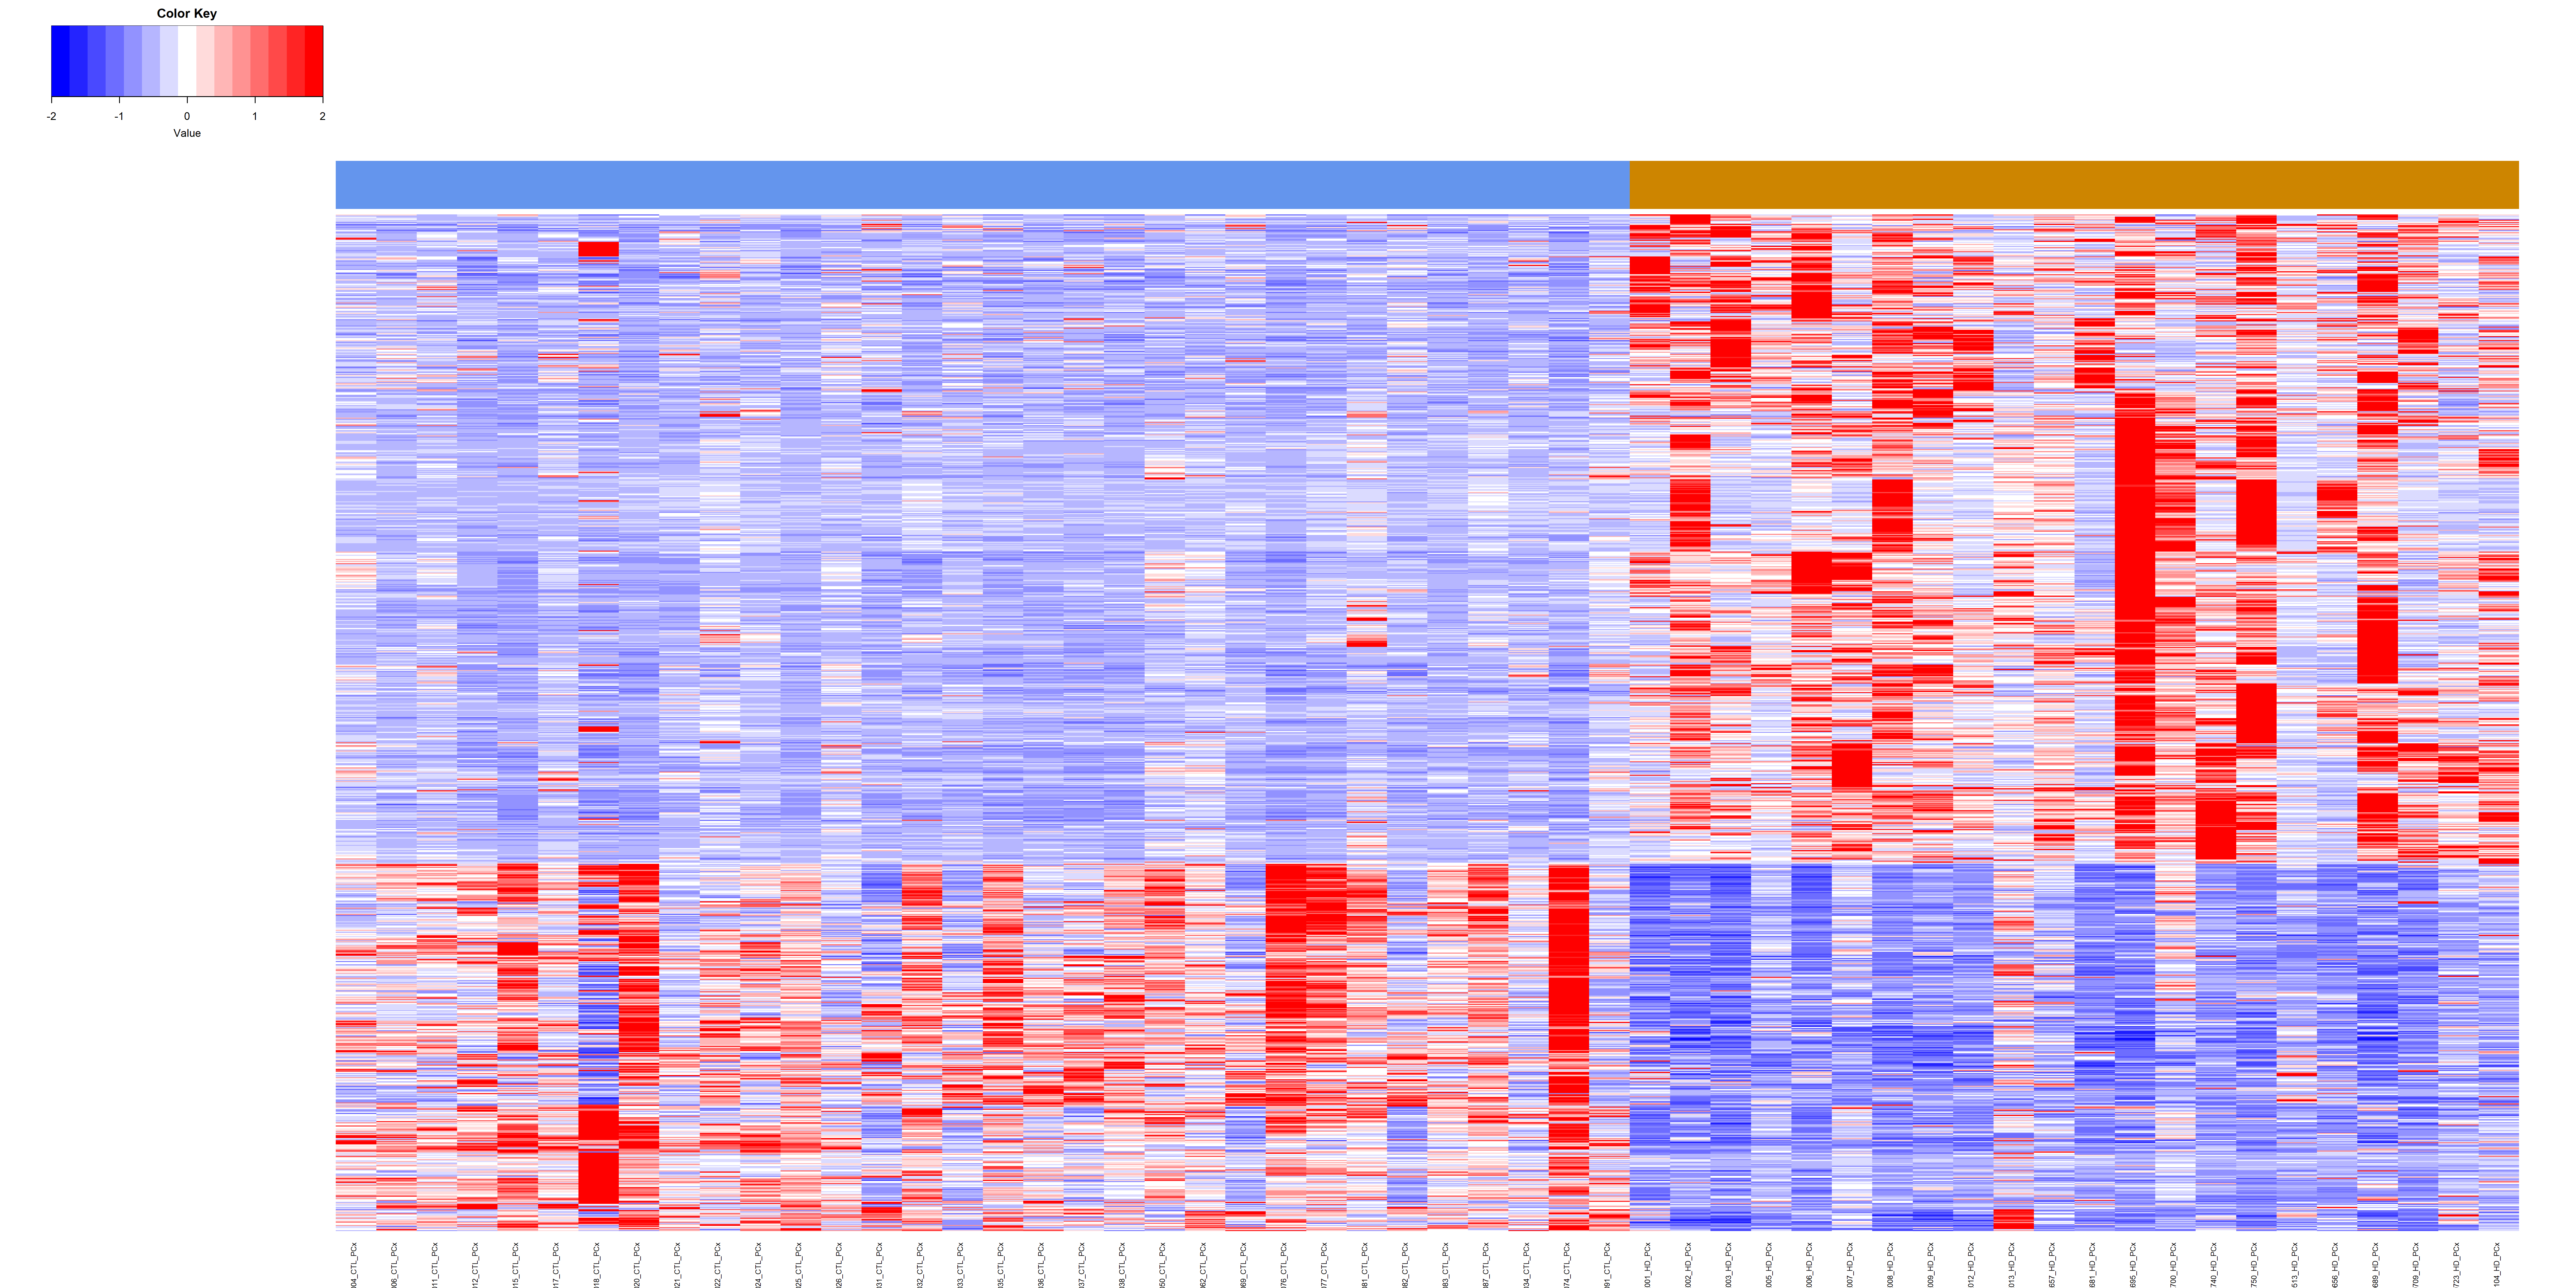
\includegraphics[width = 11cm]{Figures/DE heatmap/CTLvsHD-PCx_all.png}}
\caption{Heatmap of PCx-HD dataset for all the differentially expressed genes.}
\label{DE-pcx-hd}
\footnotesize $|$LFC$| >$ 1; HD is the contrast reference. Blue bar: control samples; golden bar: HD samples.
\end{figure}

%\section{Heatmaps for Blood-HD-f comparisons} 

\begin{figure}[!ht]
    \centerline{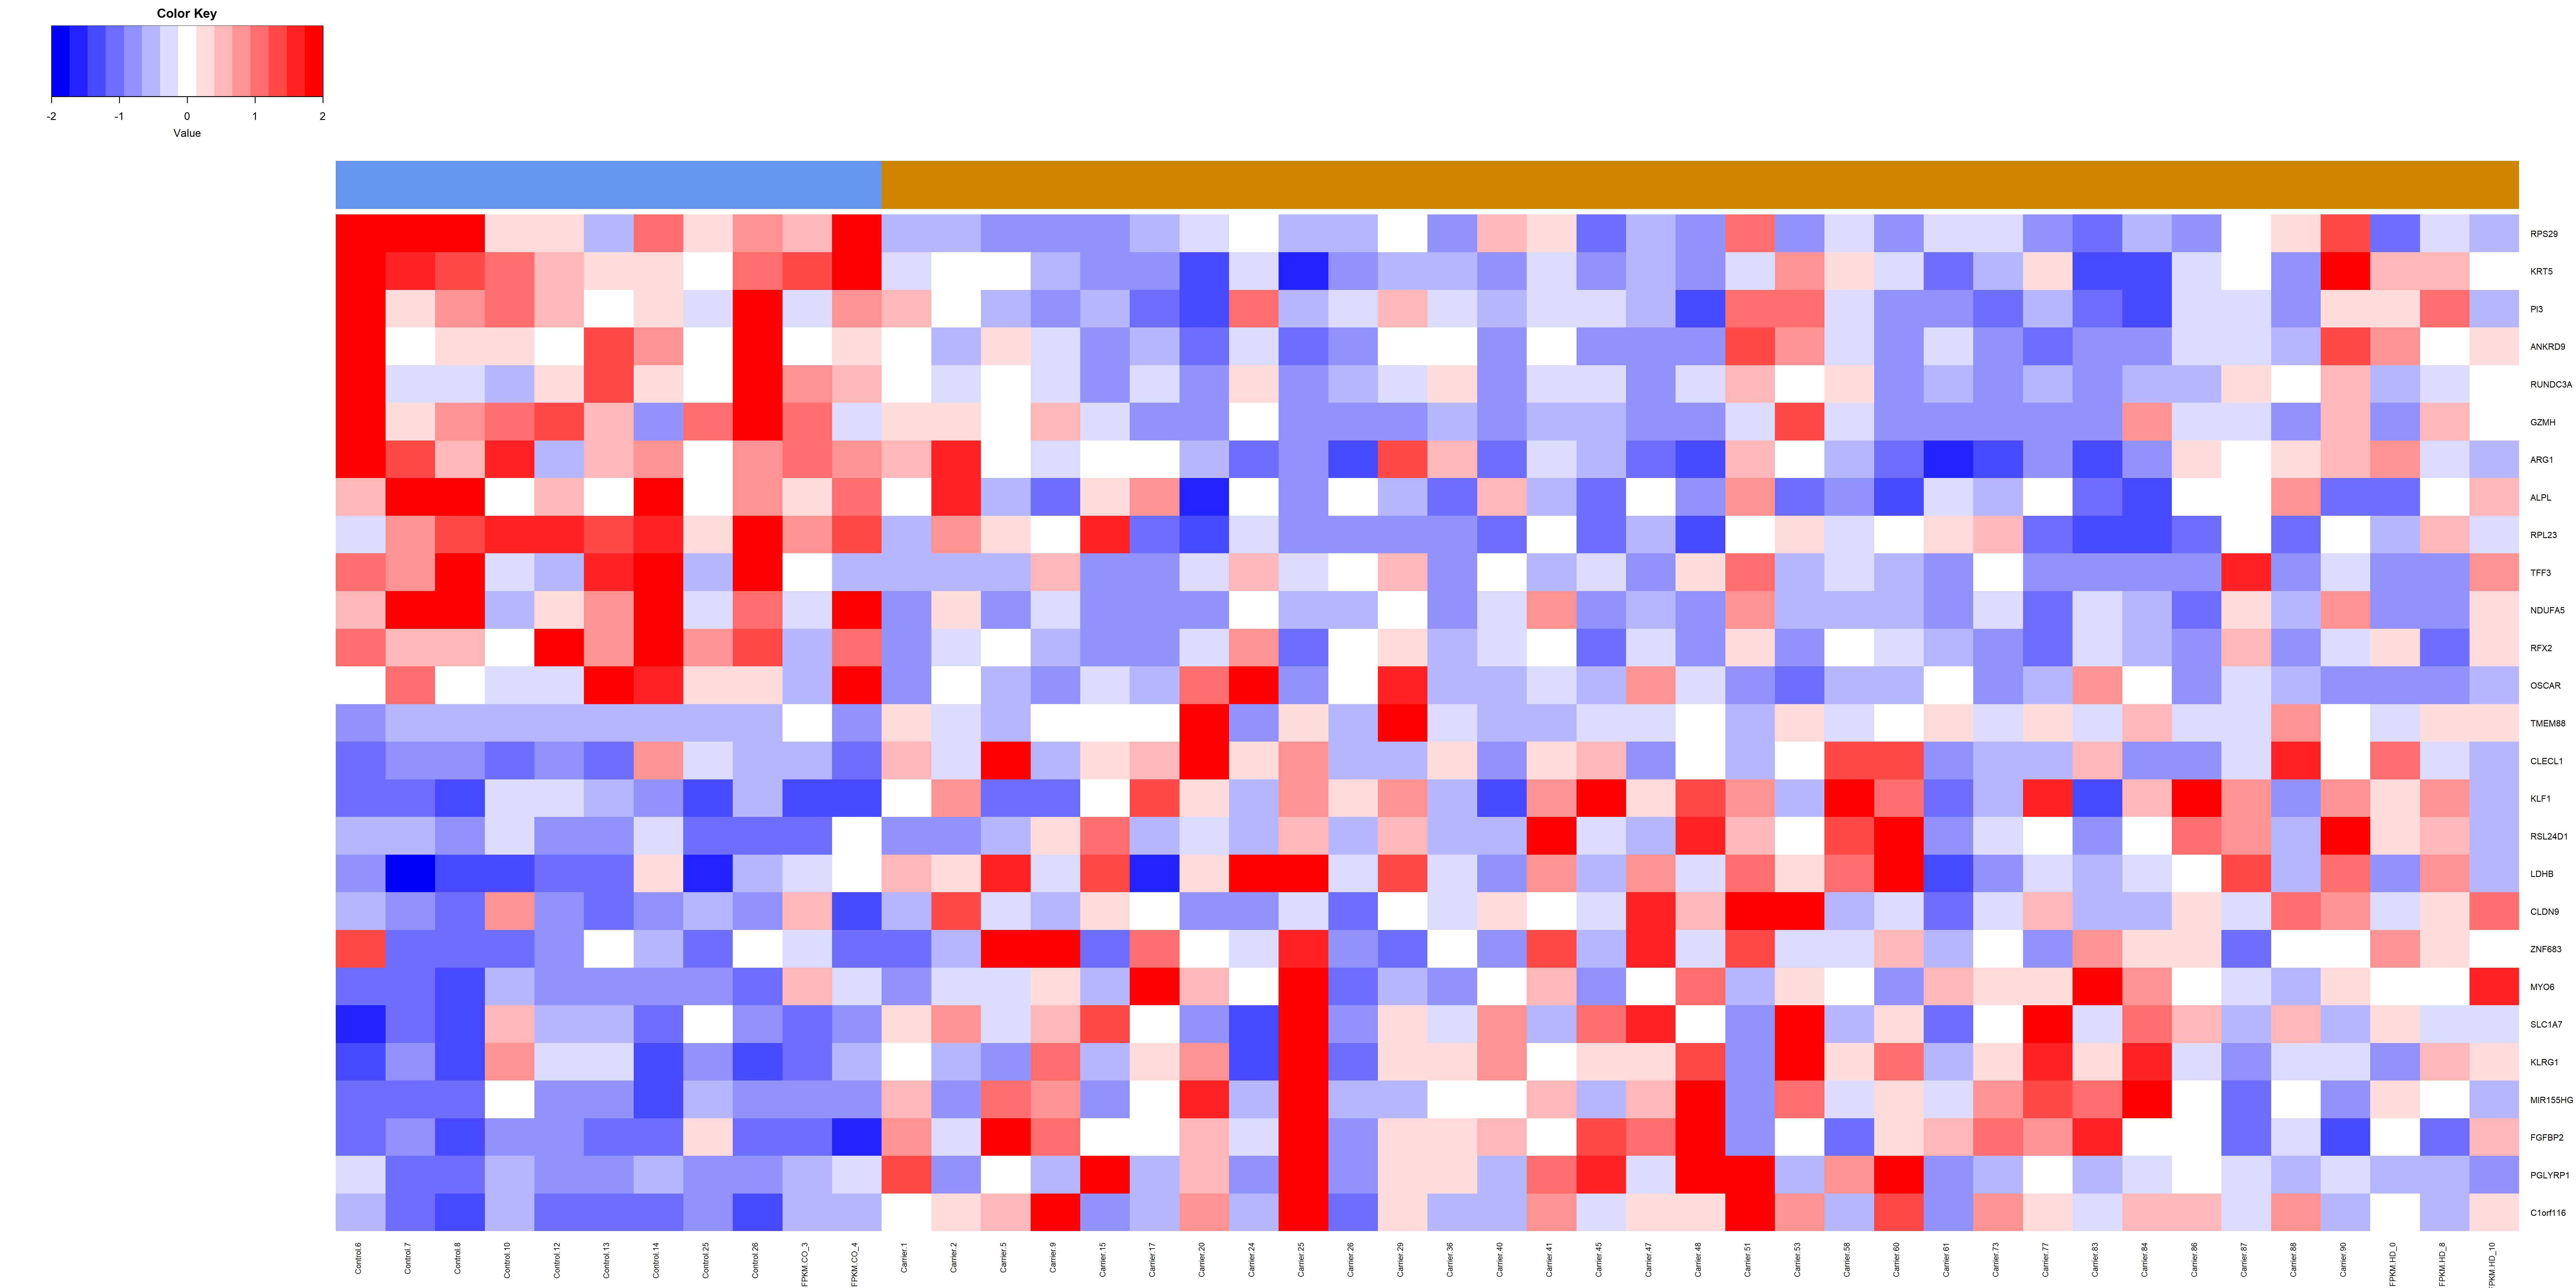
\includegraphics[width = 11cm]{Figures/DE heatmap/CTLvsHD-Blood-f_27.png}}
\caption{Heatmap of Blood-HD-f dataset for all the differentially expressed genes (27 genes).}
\label{DE-blood-hd-f}
\footnotesize $|$LFC$| >$ 1; HD is the contrast reference. Blue bar: control samples; golden bar: HD samples.
\end{figure}

\begin{figure}[!ht]
    \centerline{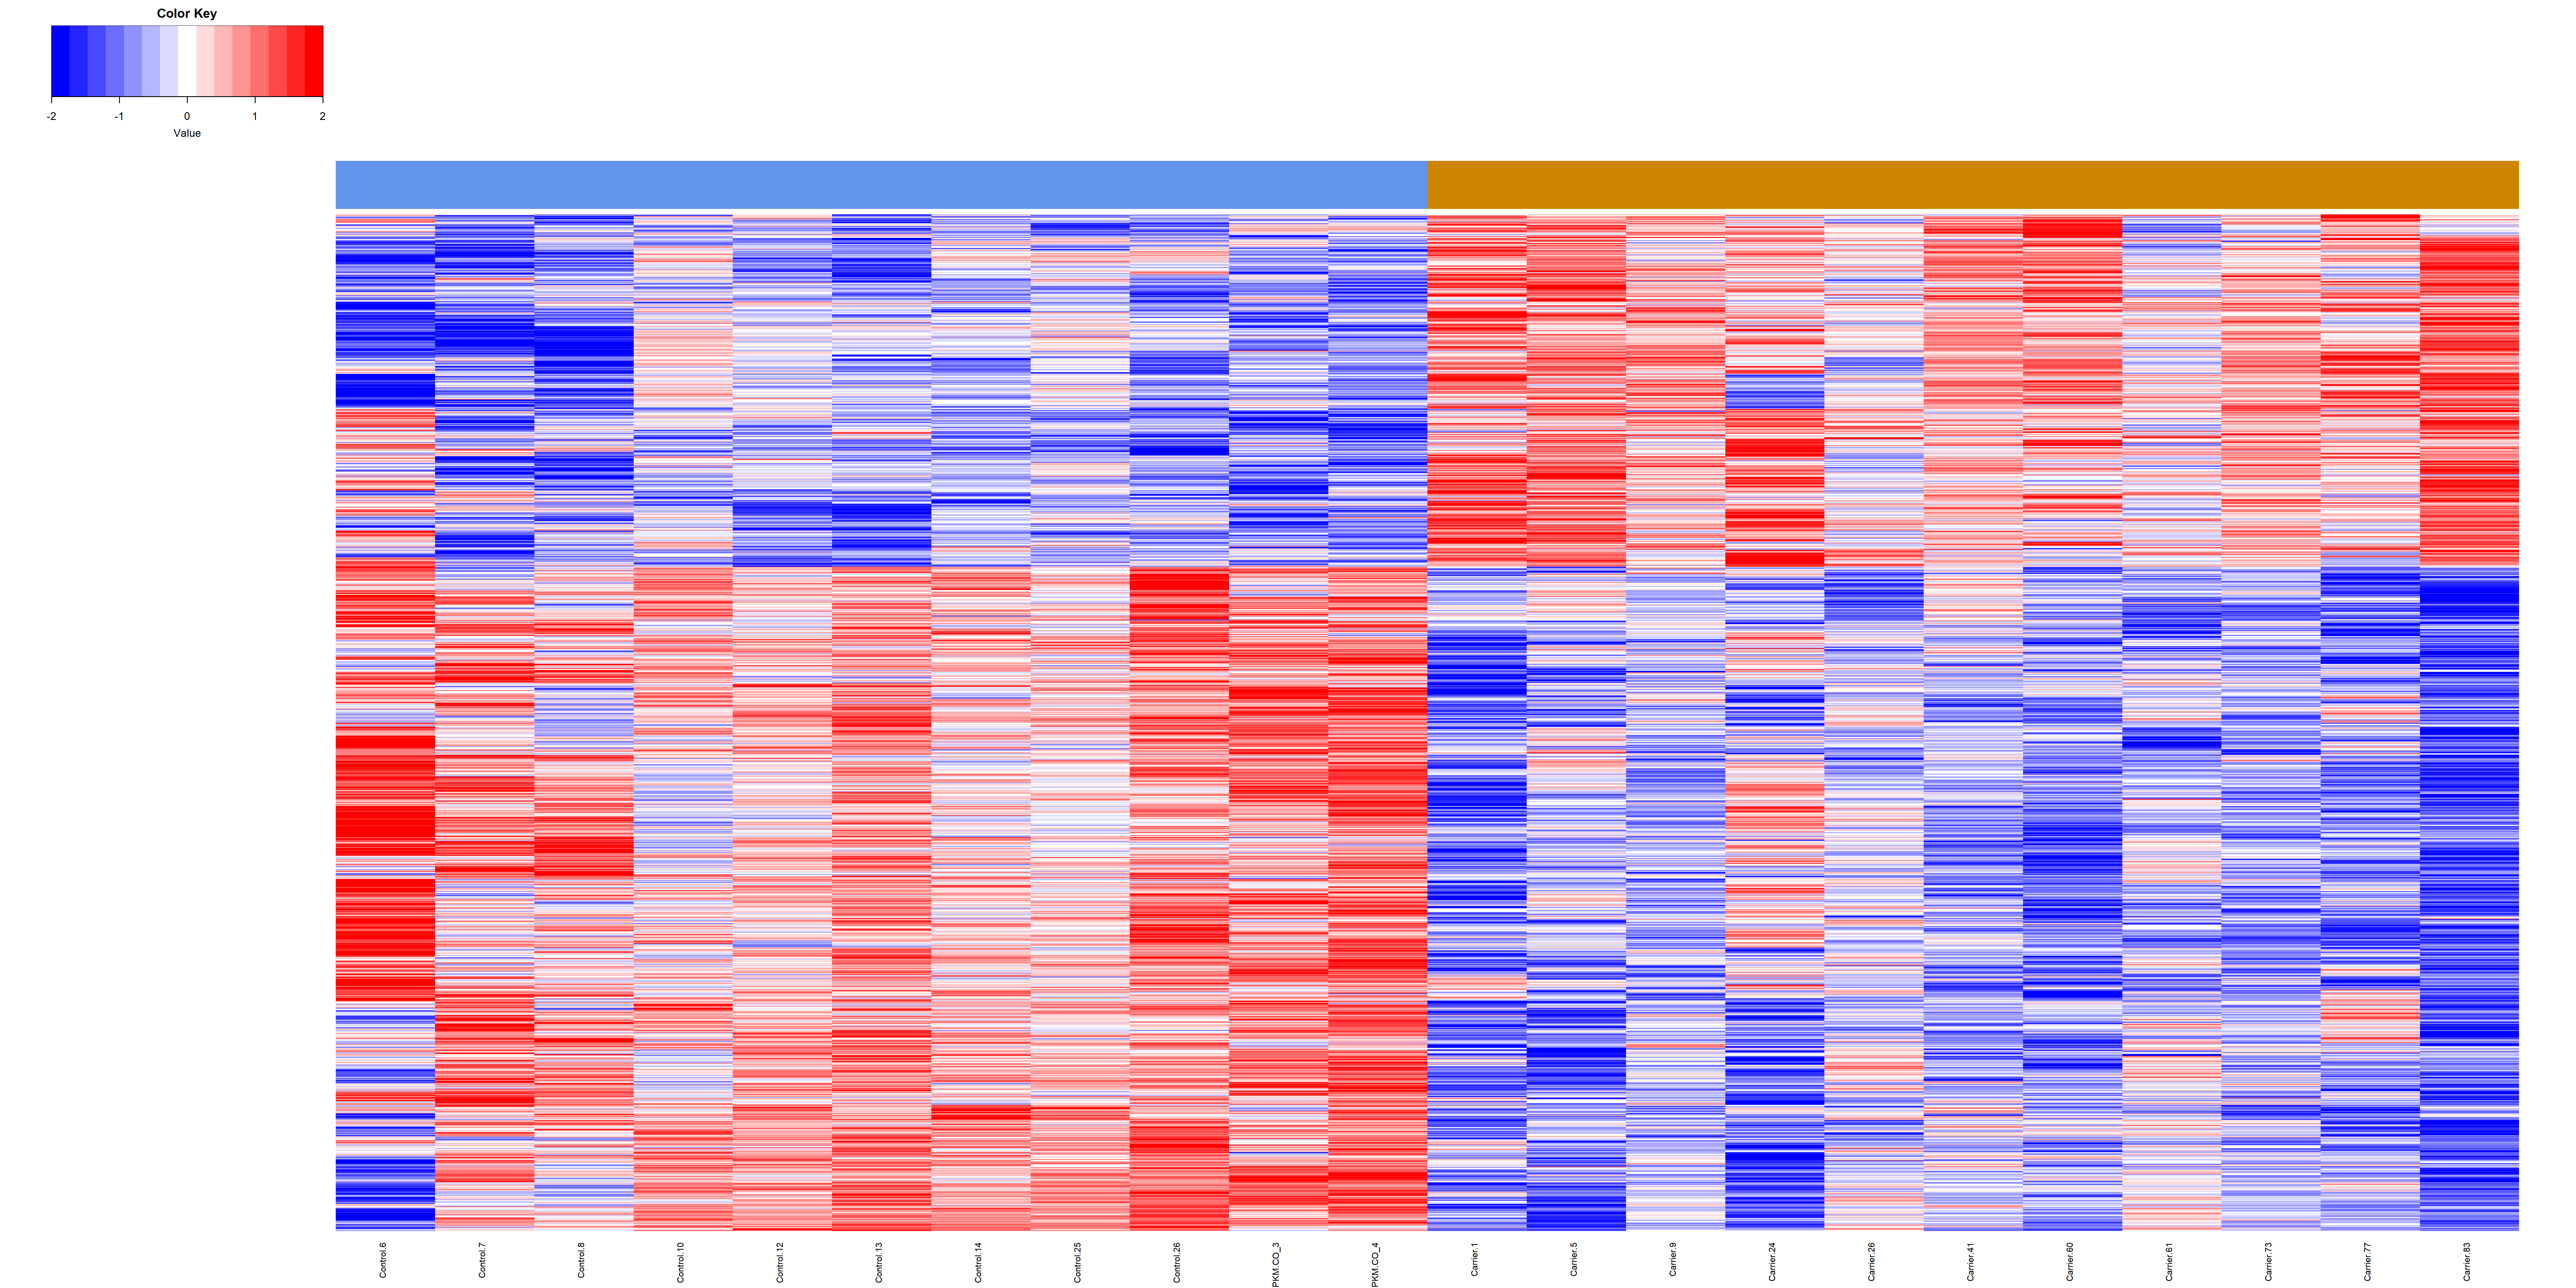
\includegraphics[width = 11cm]{Figures/DE heatmap/CTLvs1_HD-Blood-f_all.png}}
\caption{Heatmap of Blood-HD-f dataset for all the differentially expressed genes between control and subtype 1.}
\footnotesize $|$LFC$| >$ 1; case is the contrast reference. Blue bar: control samples; golden bar: S1 samples.
\end{figure}

\begin{figure}[!ht]
    \centerline{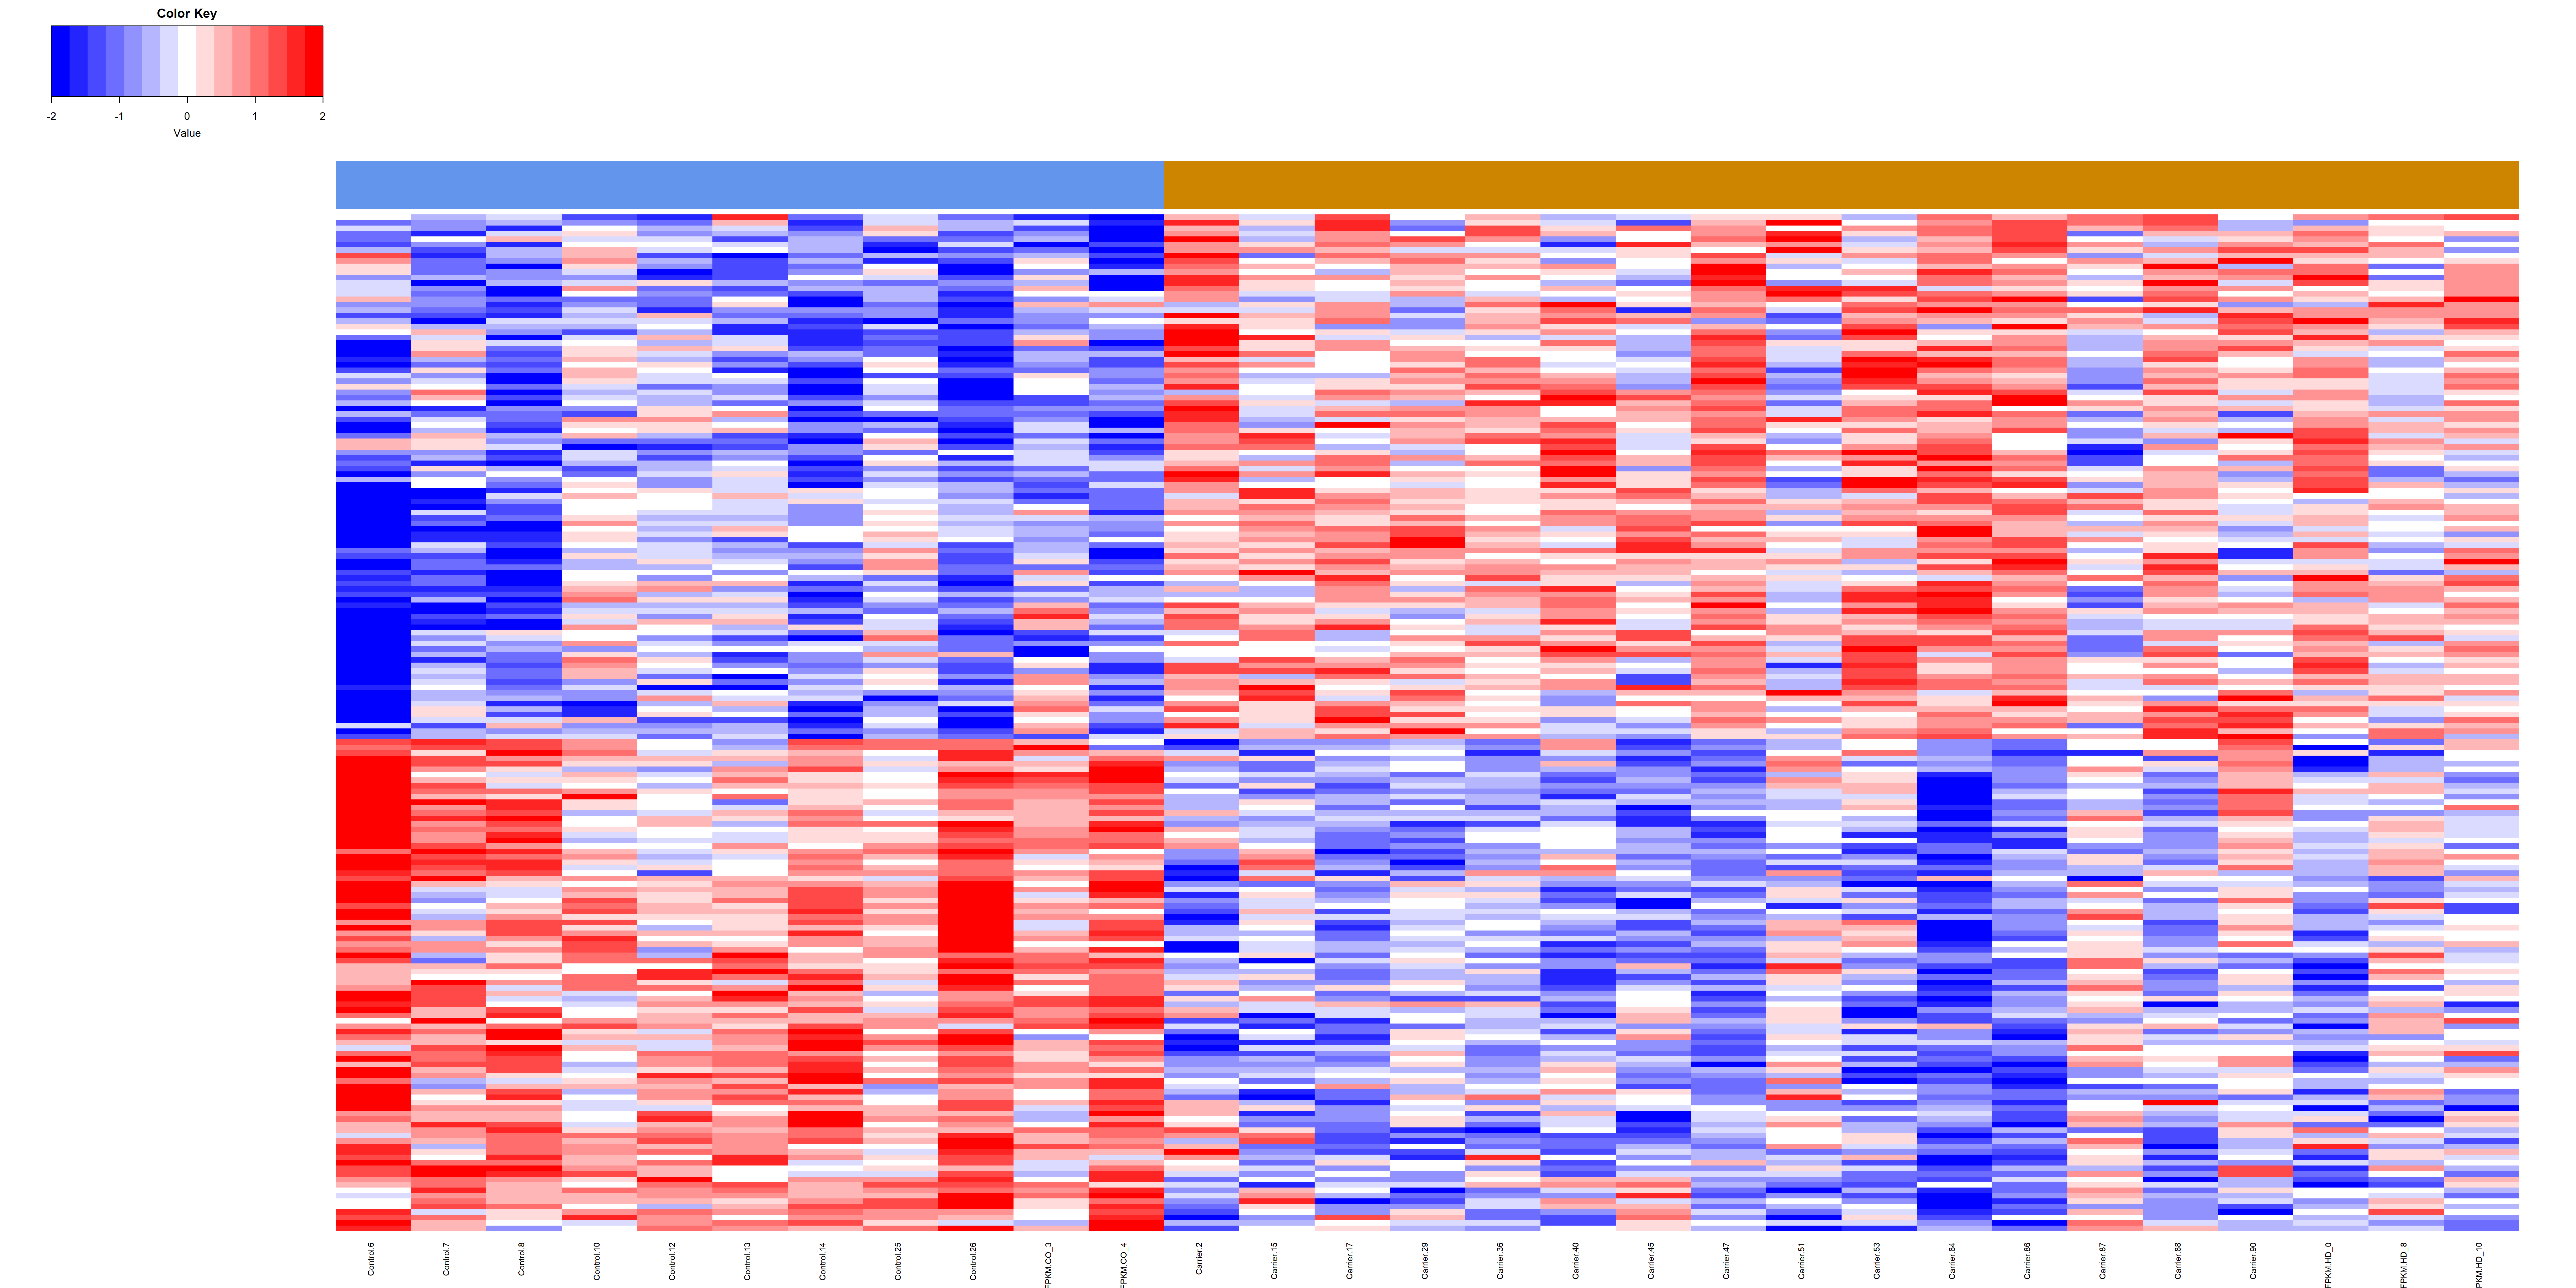
\includegraphics[width = 11cm]{Figures/DE heatmap/CTLvs2_HD-Blood-f_all.png}}
\caption{Heatmap of Blood-HD-f dataset for all the differentially expressed genes between control and subtype 2.}
\footnotesize $|$LFC$| >$ 1; case is the contrast reference. Blue bar: control samples; golden bar: S2 samples.
\end{figure}

\begin{figure}[!ht]
    \centerline{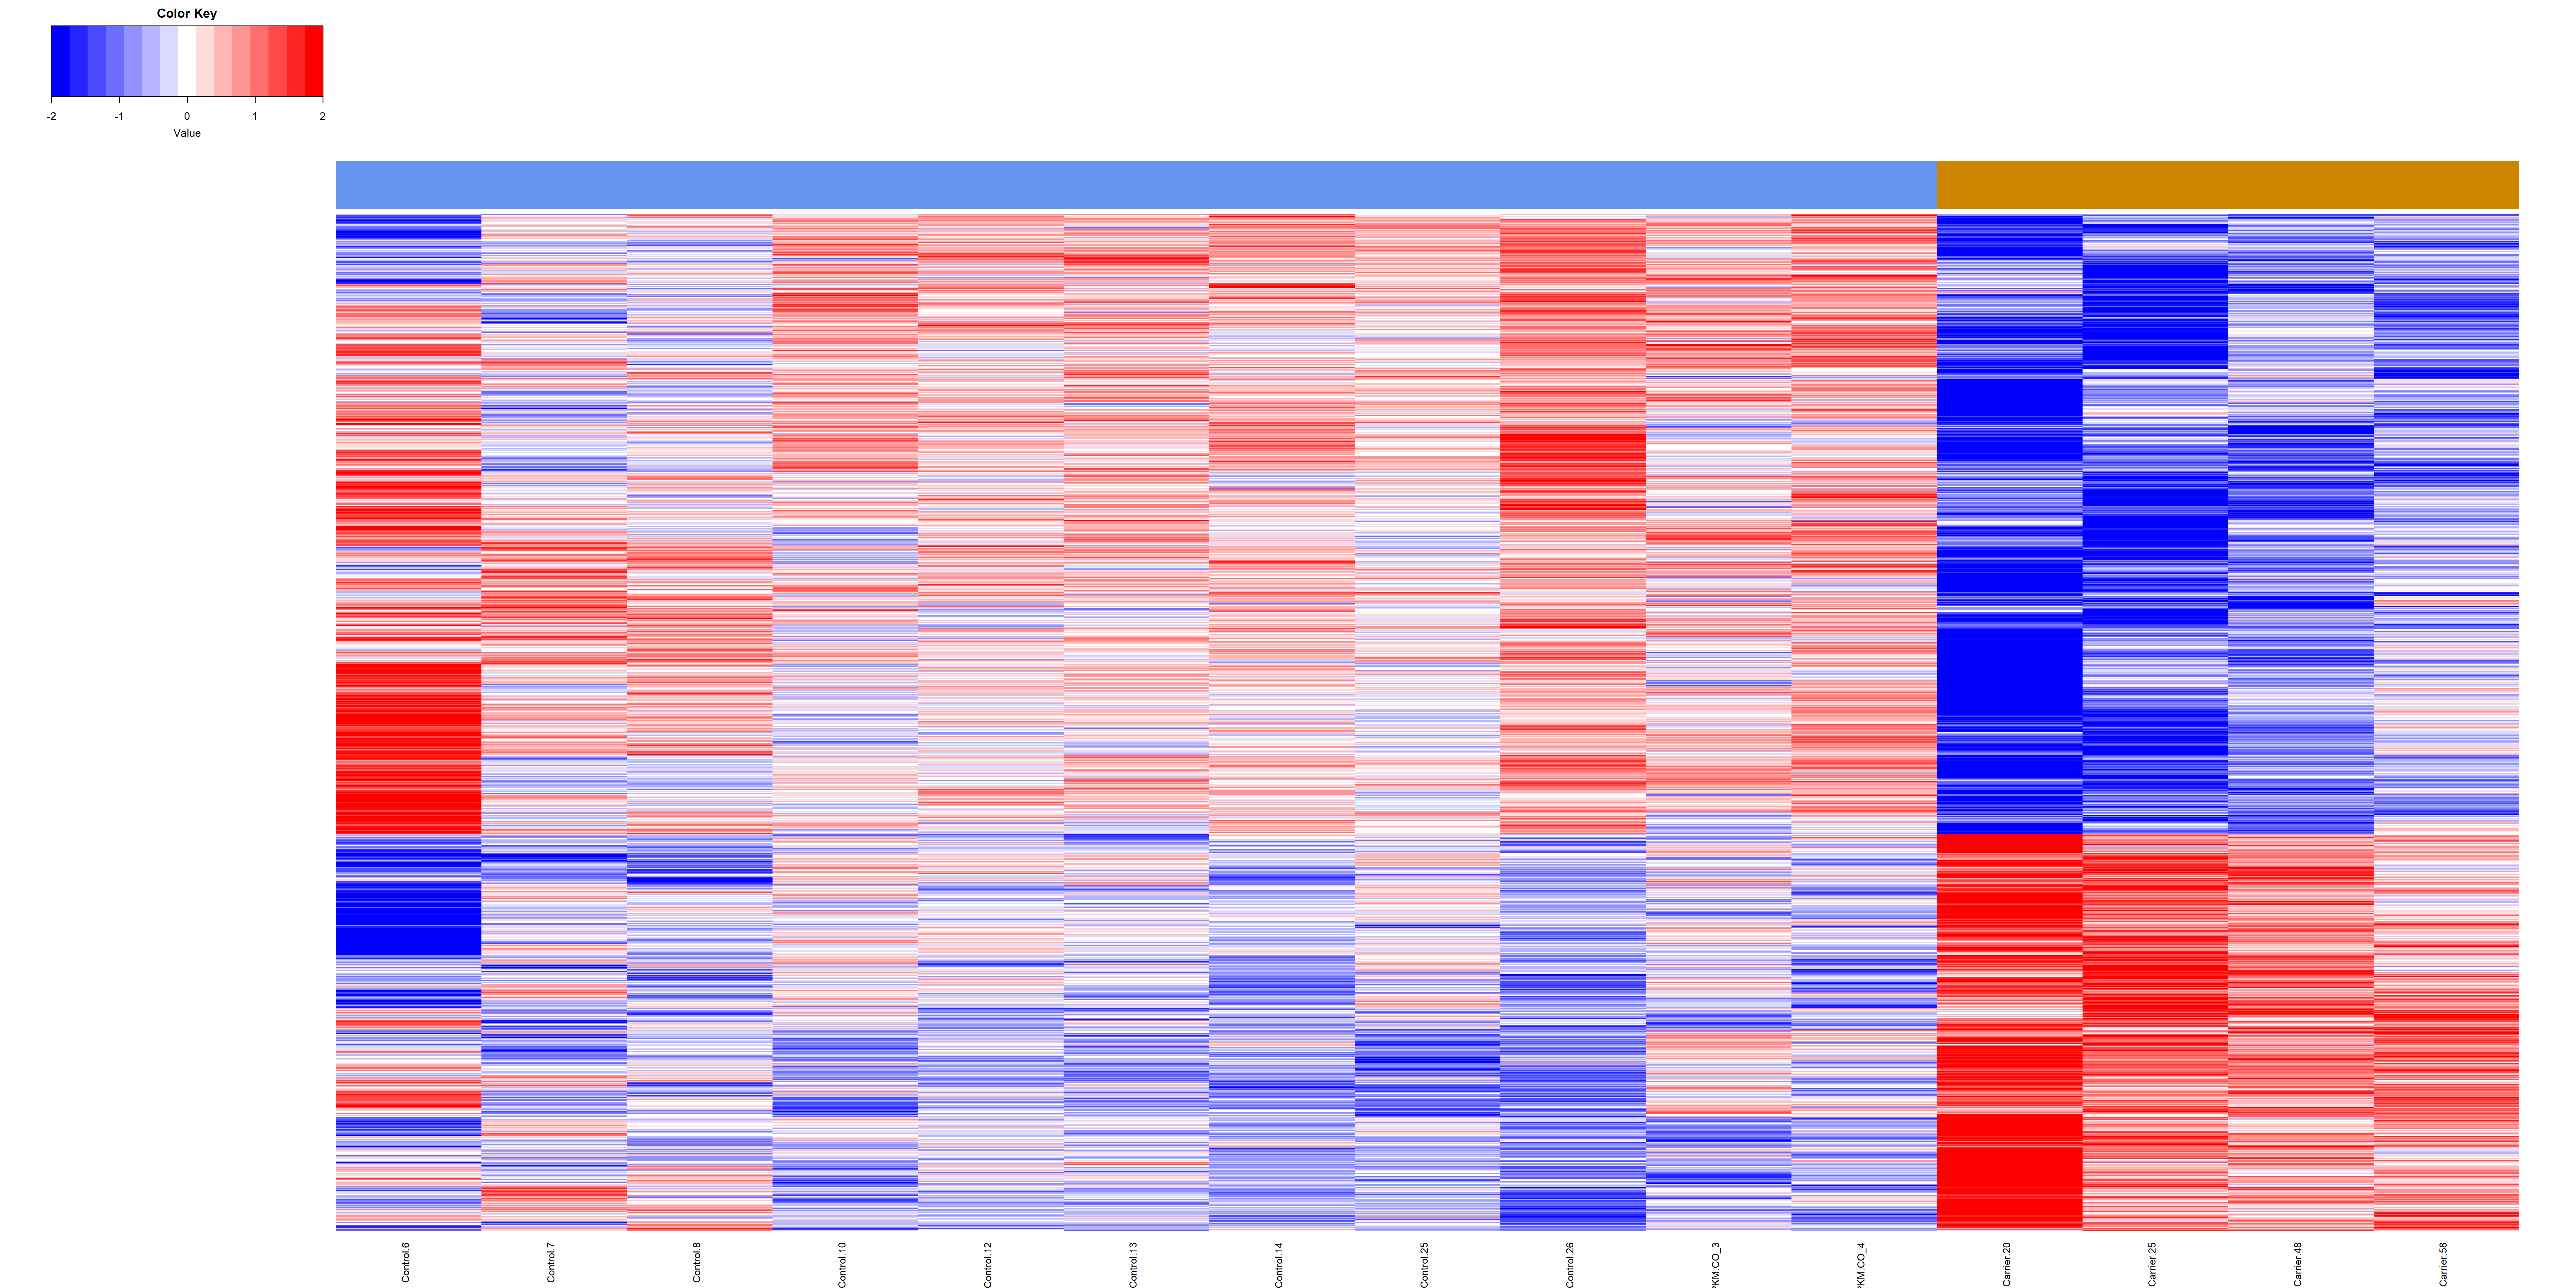
\includegraphics[width = 11cm]{Figures/DE heatmap/CTLvs3_HD-Blood-f_all.png}}
\caption{Heatmap of Blood-HD-f dataset for all the differentially expressed genes between control and subtype 3.}
\footnotesize $|$LFC$| >$ 1; case is the contrast reference. Blue bar: control samples; golden bar: S3 samples.
\end{figure}

%\section{Heatmaps for Blood-HD-m comparisons} 

\begin{figure}[!ht]
    \centerline{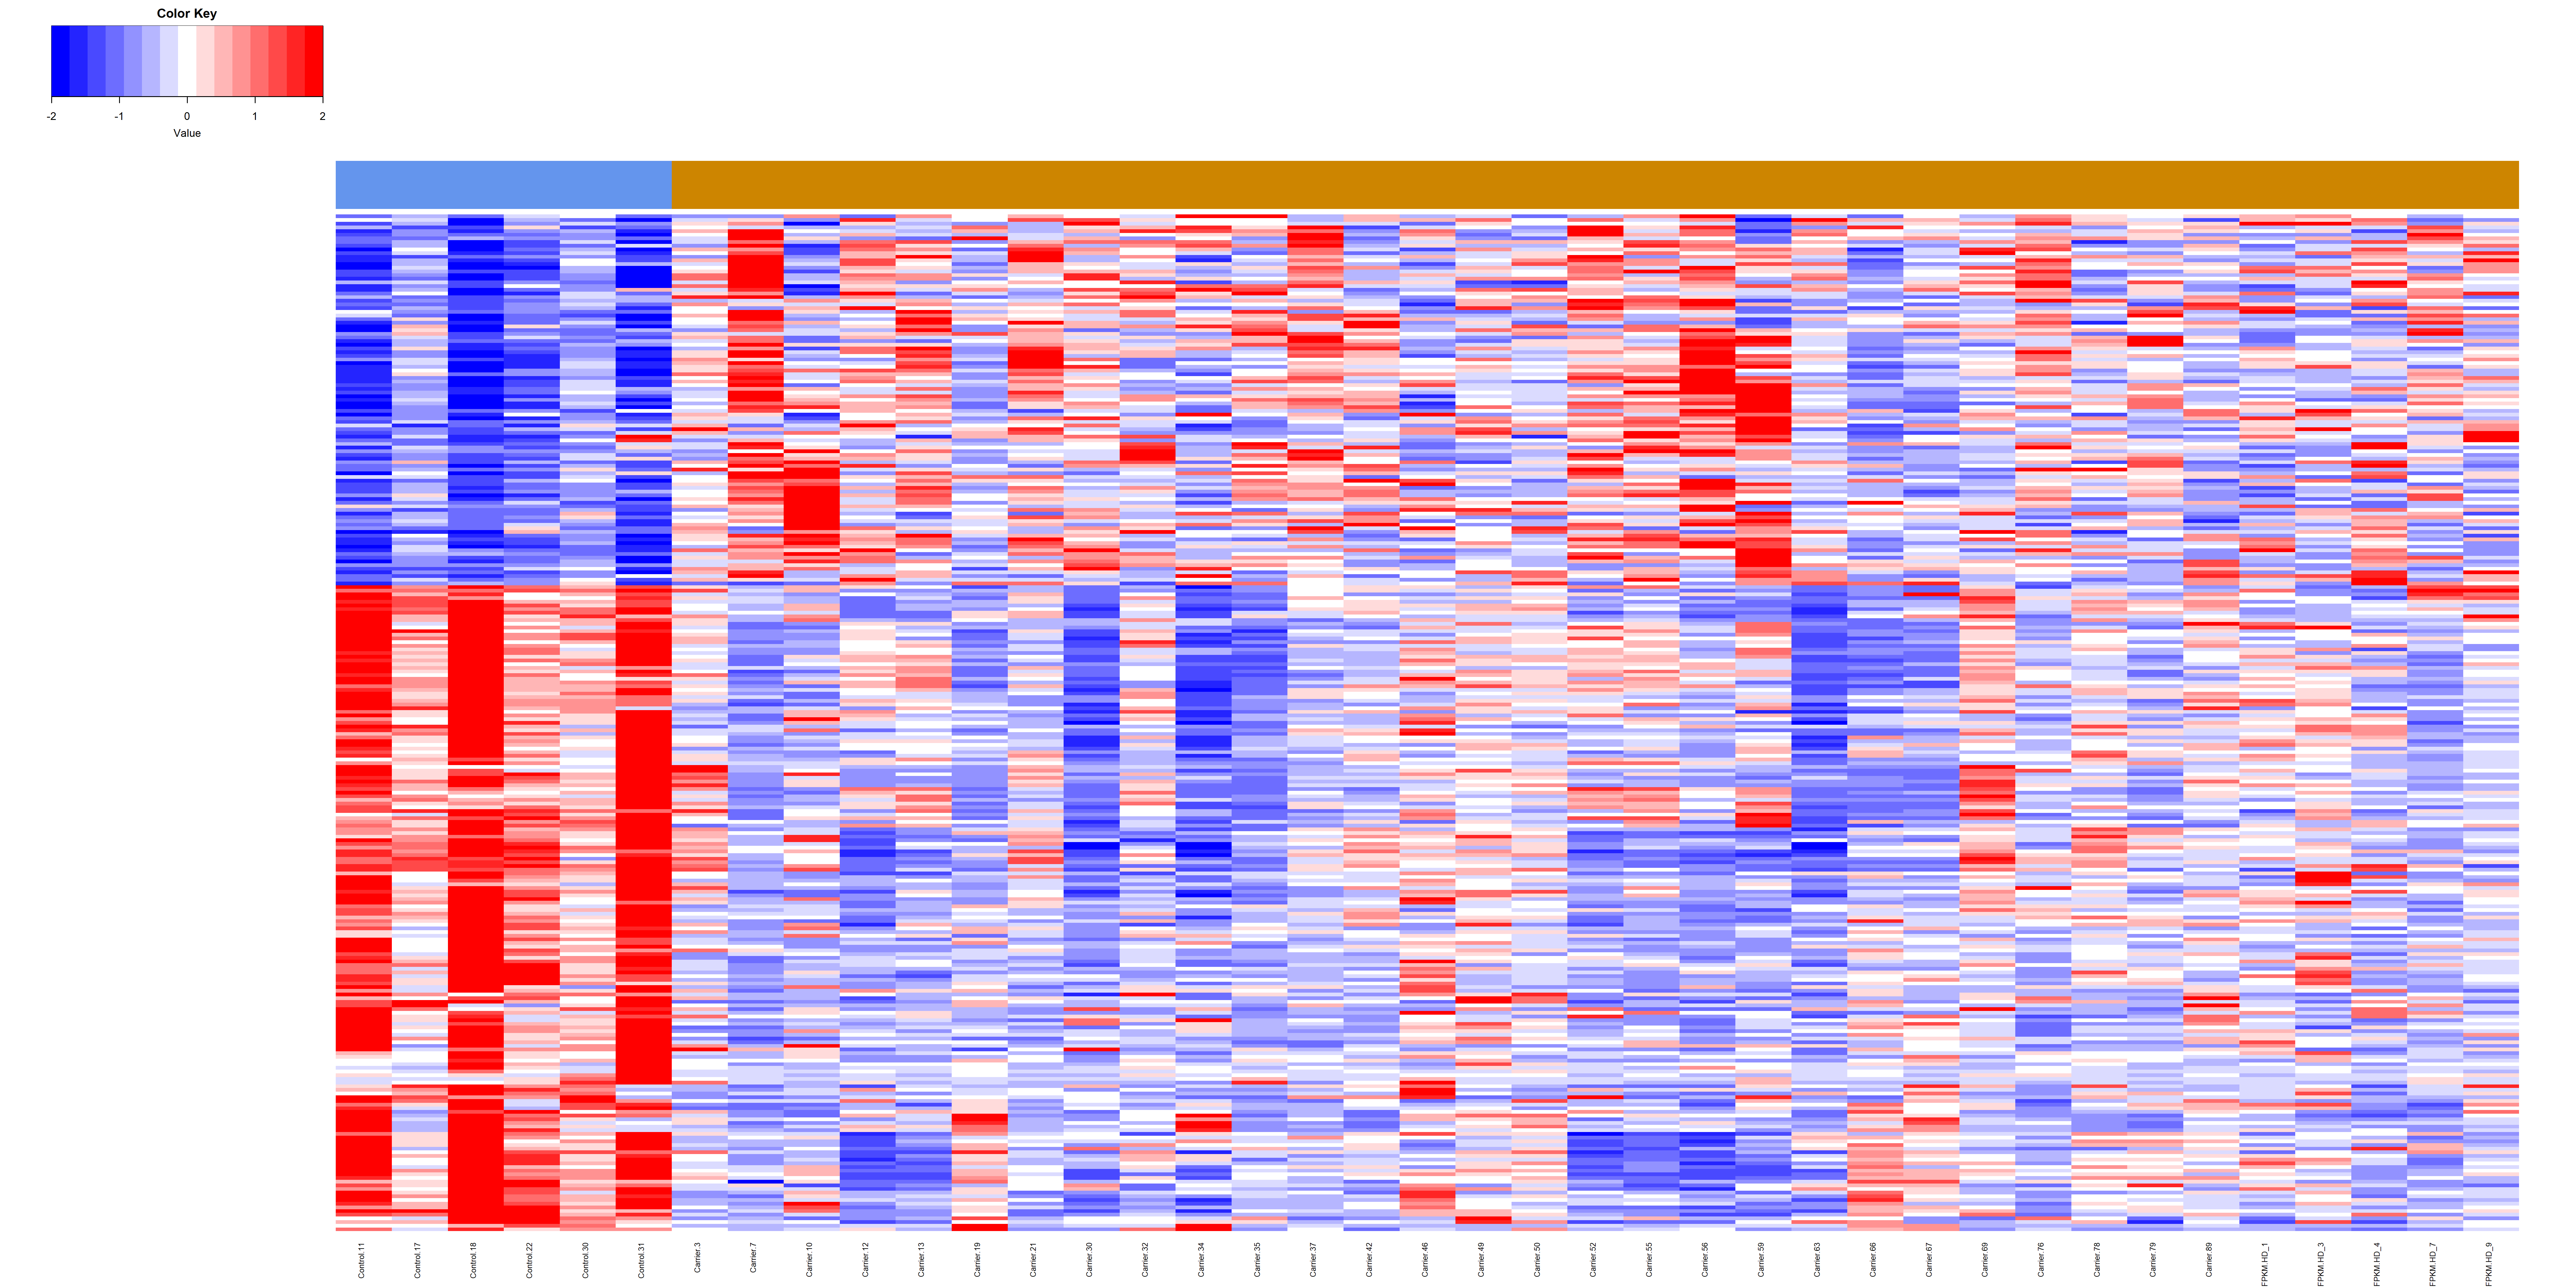
\includegraphics[width = 11cm]{Figures/DE heatmap/CTLvsHD-blood-m_all.png}}
\caption{Heatmap of Blood-HD-m dataset for all the differentially expressed genes.}
\label{DE-blood-hd-m}
\footnotesize $|$LFC$| >$ 1; HD is the contrast reference. Blue bar: control samples; golden bar: HD samples.
\end{figure}

\begin{figure}[!ht]
    \centerline{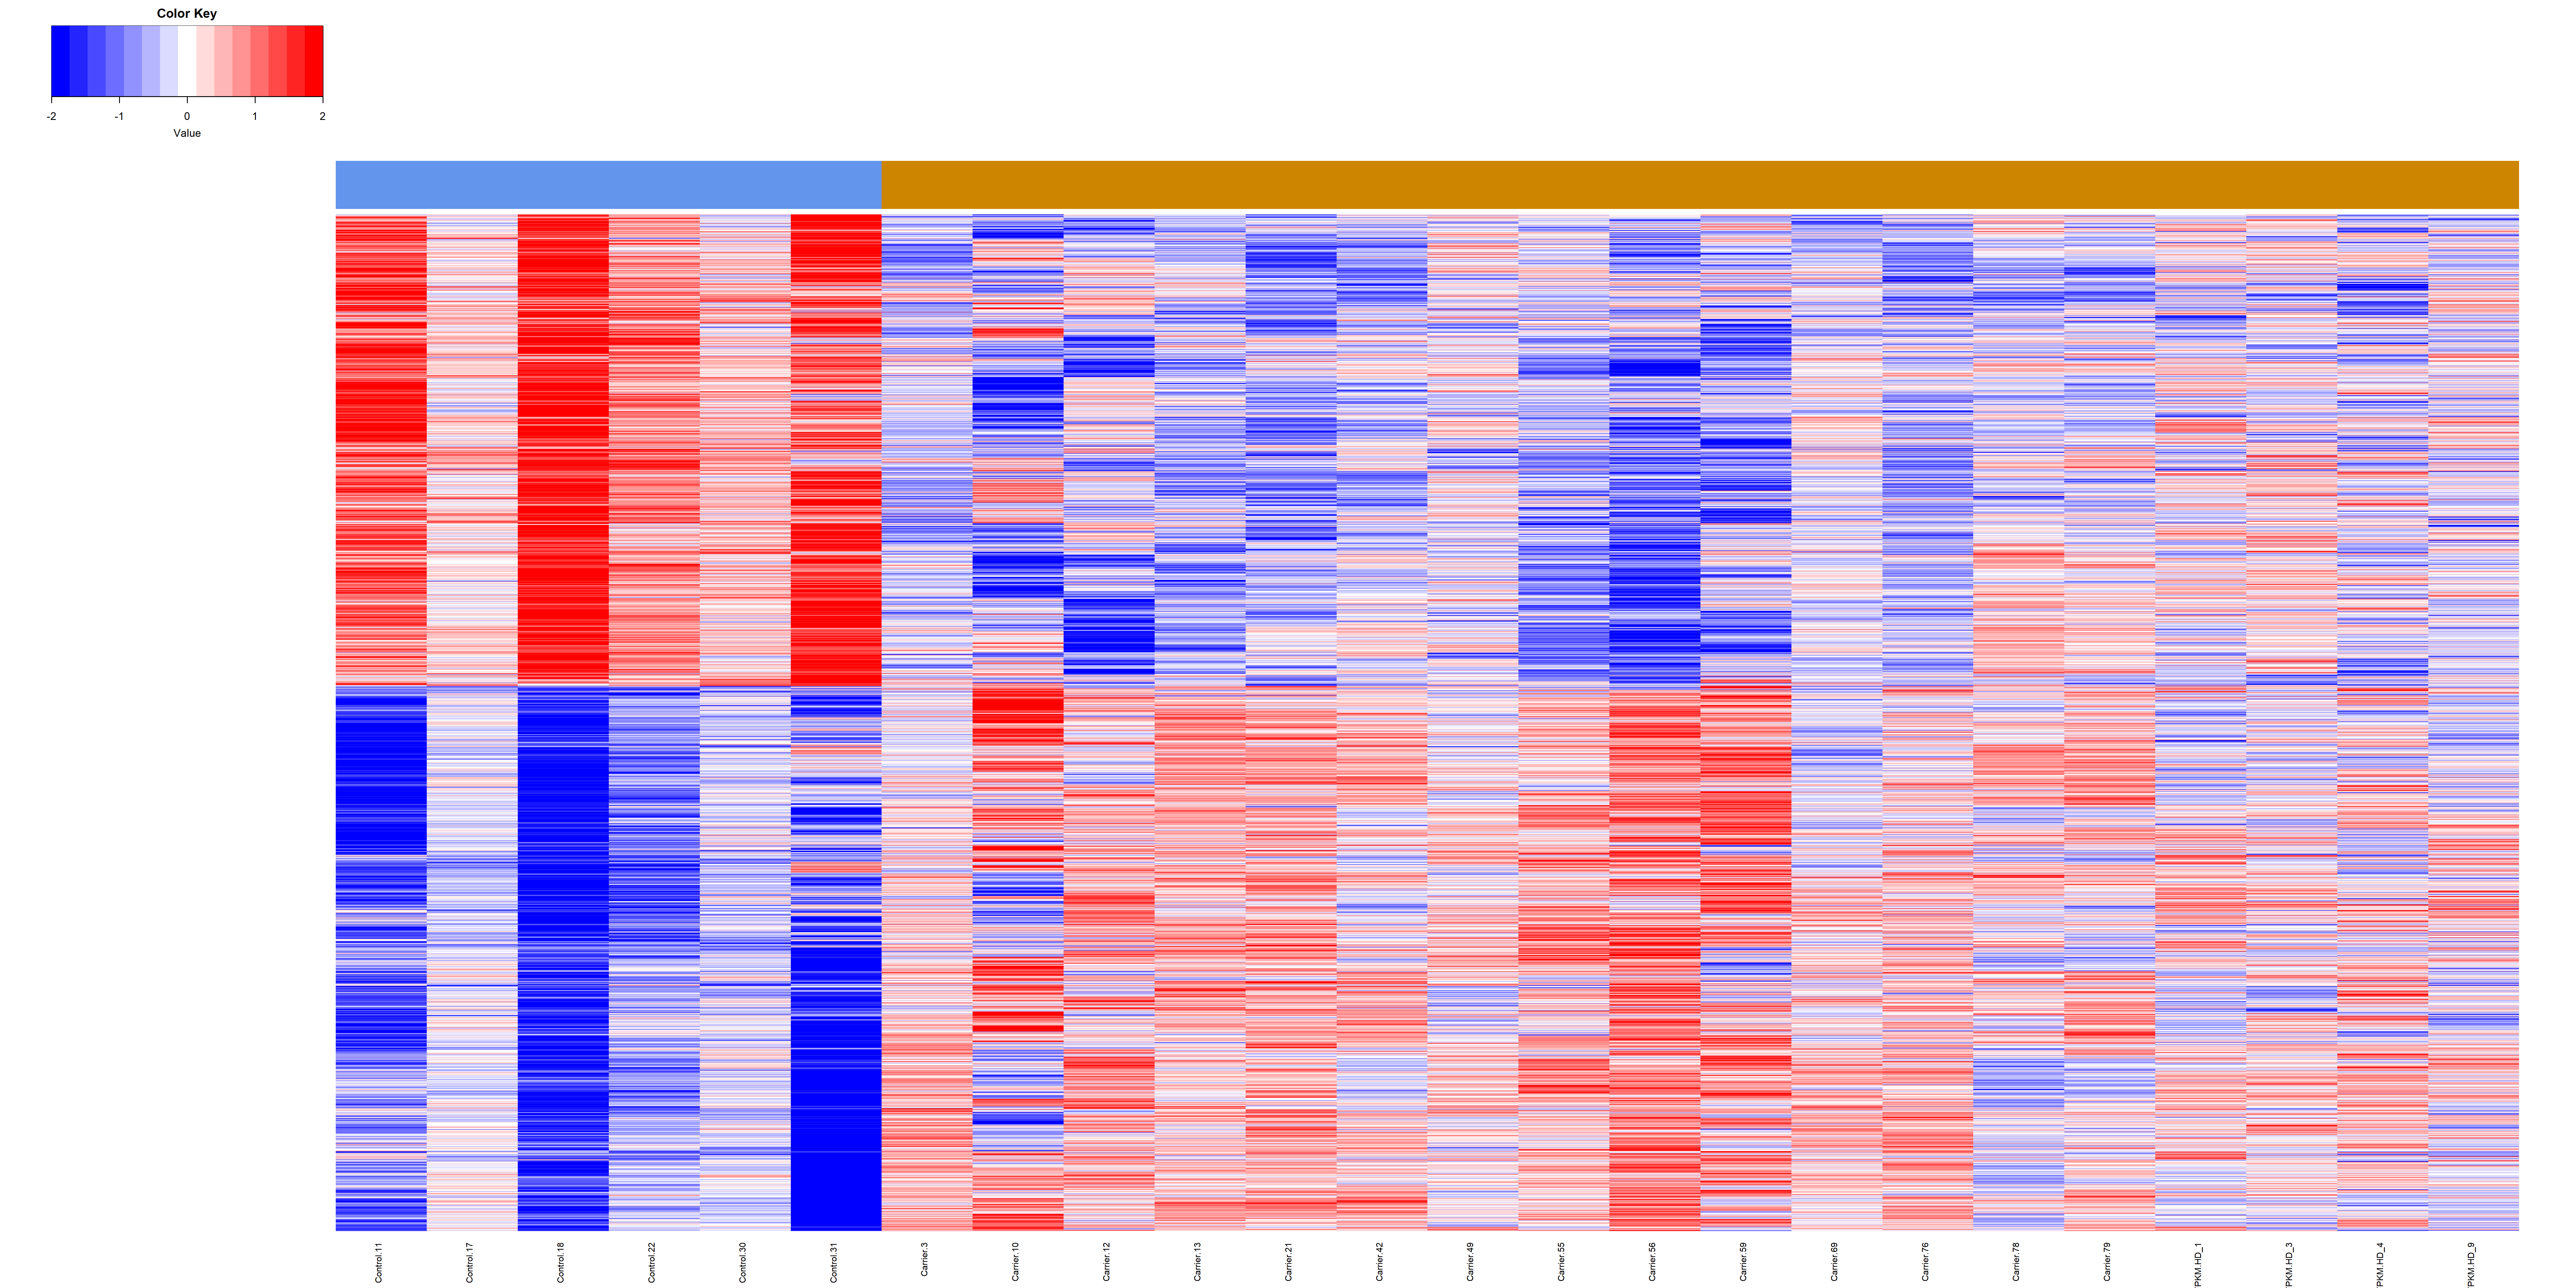
\includegraphics[width = 11cm]{Figures/DE heatmap/CTLvs1_HD-Blood-m_all.png}}
\caption{Heatmap of Blood-HD-m dataset for all the differentially expressed genes between control and sutbype 1.}
\footnotesize $|$LFC$| >$ 1.25; case is the contrast reference. Blue bar: control samples; golden bar: S1 samples.
\end{figure}

\begin{figure}[!ht]
    \centerline{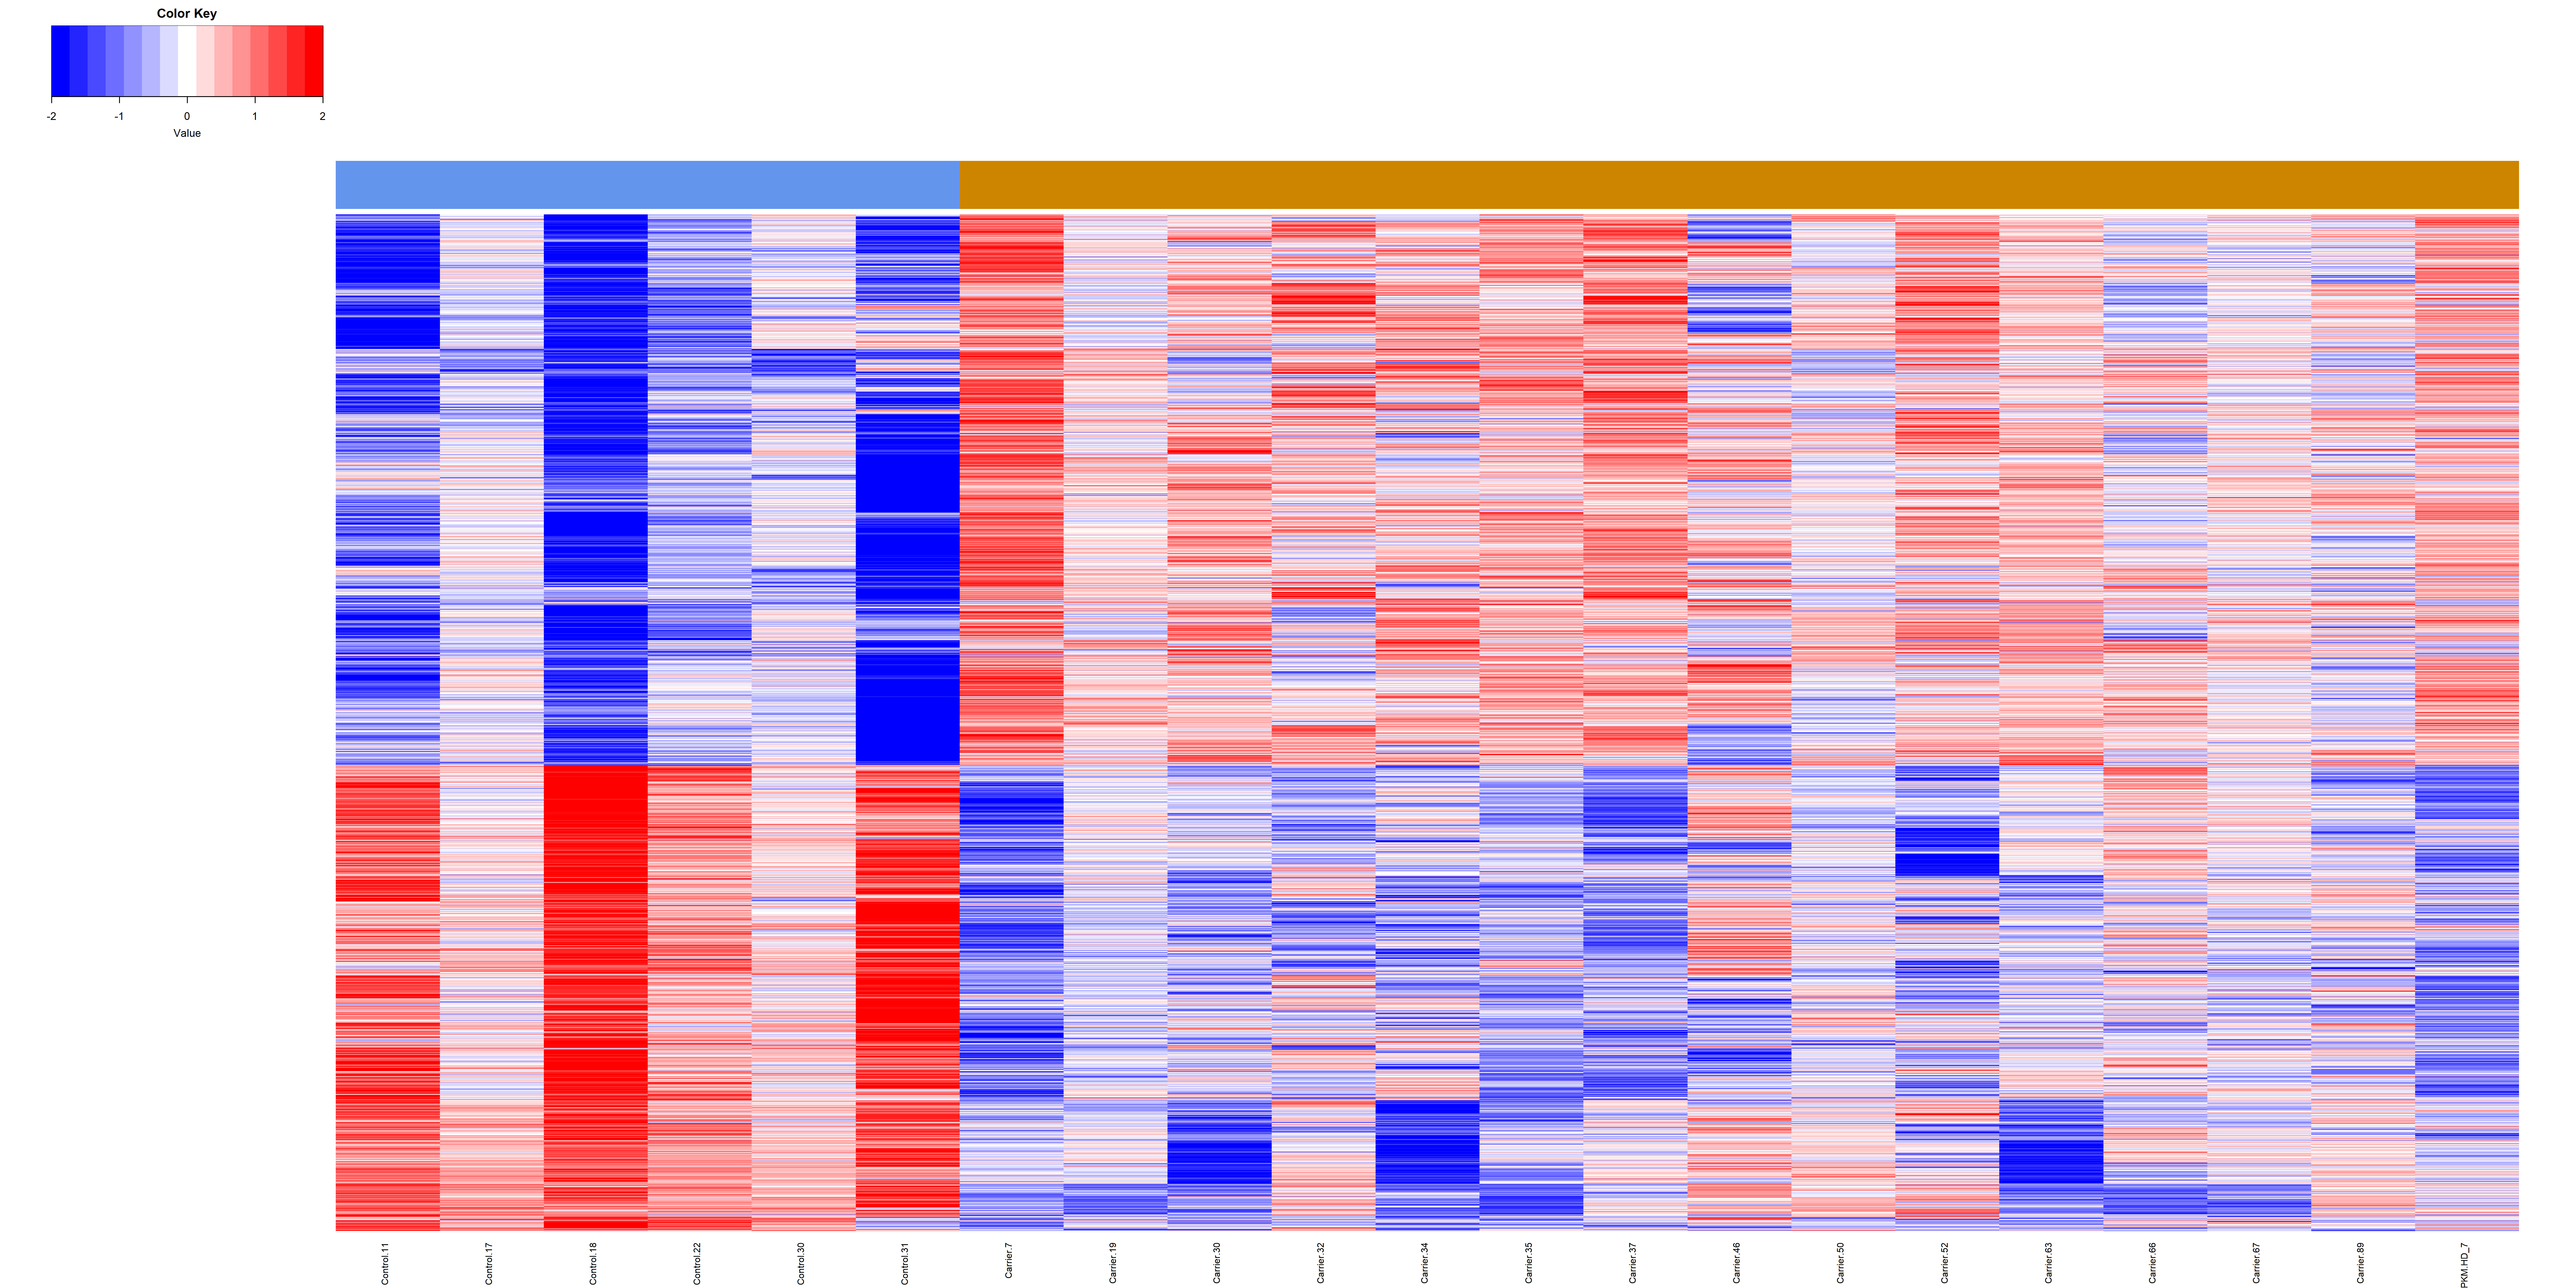
\includegraphics[width = 11cm]{Figures/DE heatmap/CTLvs2_HD-Blood-m_all.png}}
\caption{Heatmap of Blood-HD-m dataset for all the differentially expressed genes between control and sutbype 2.}
\footnotesize $|$LFC$| >$ 1.25; case is the contrast reference. Blue bar: control samples; golden bar: S2 samples.
\end{figure}

%\section{Heatmaps for Pa-AD-f comparisons}

\begin{figure}[!ht]
    \centerline{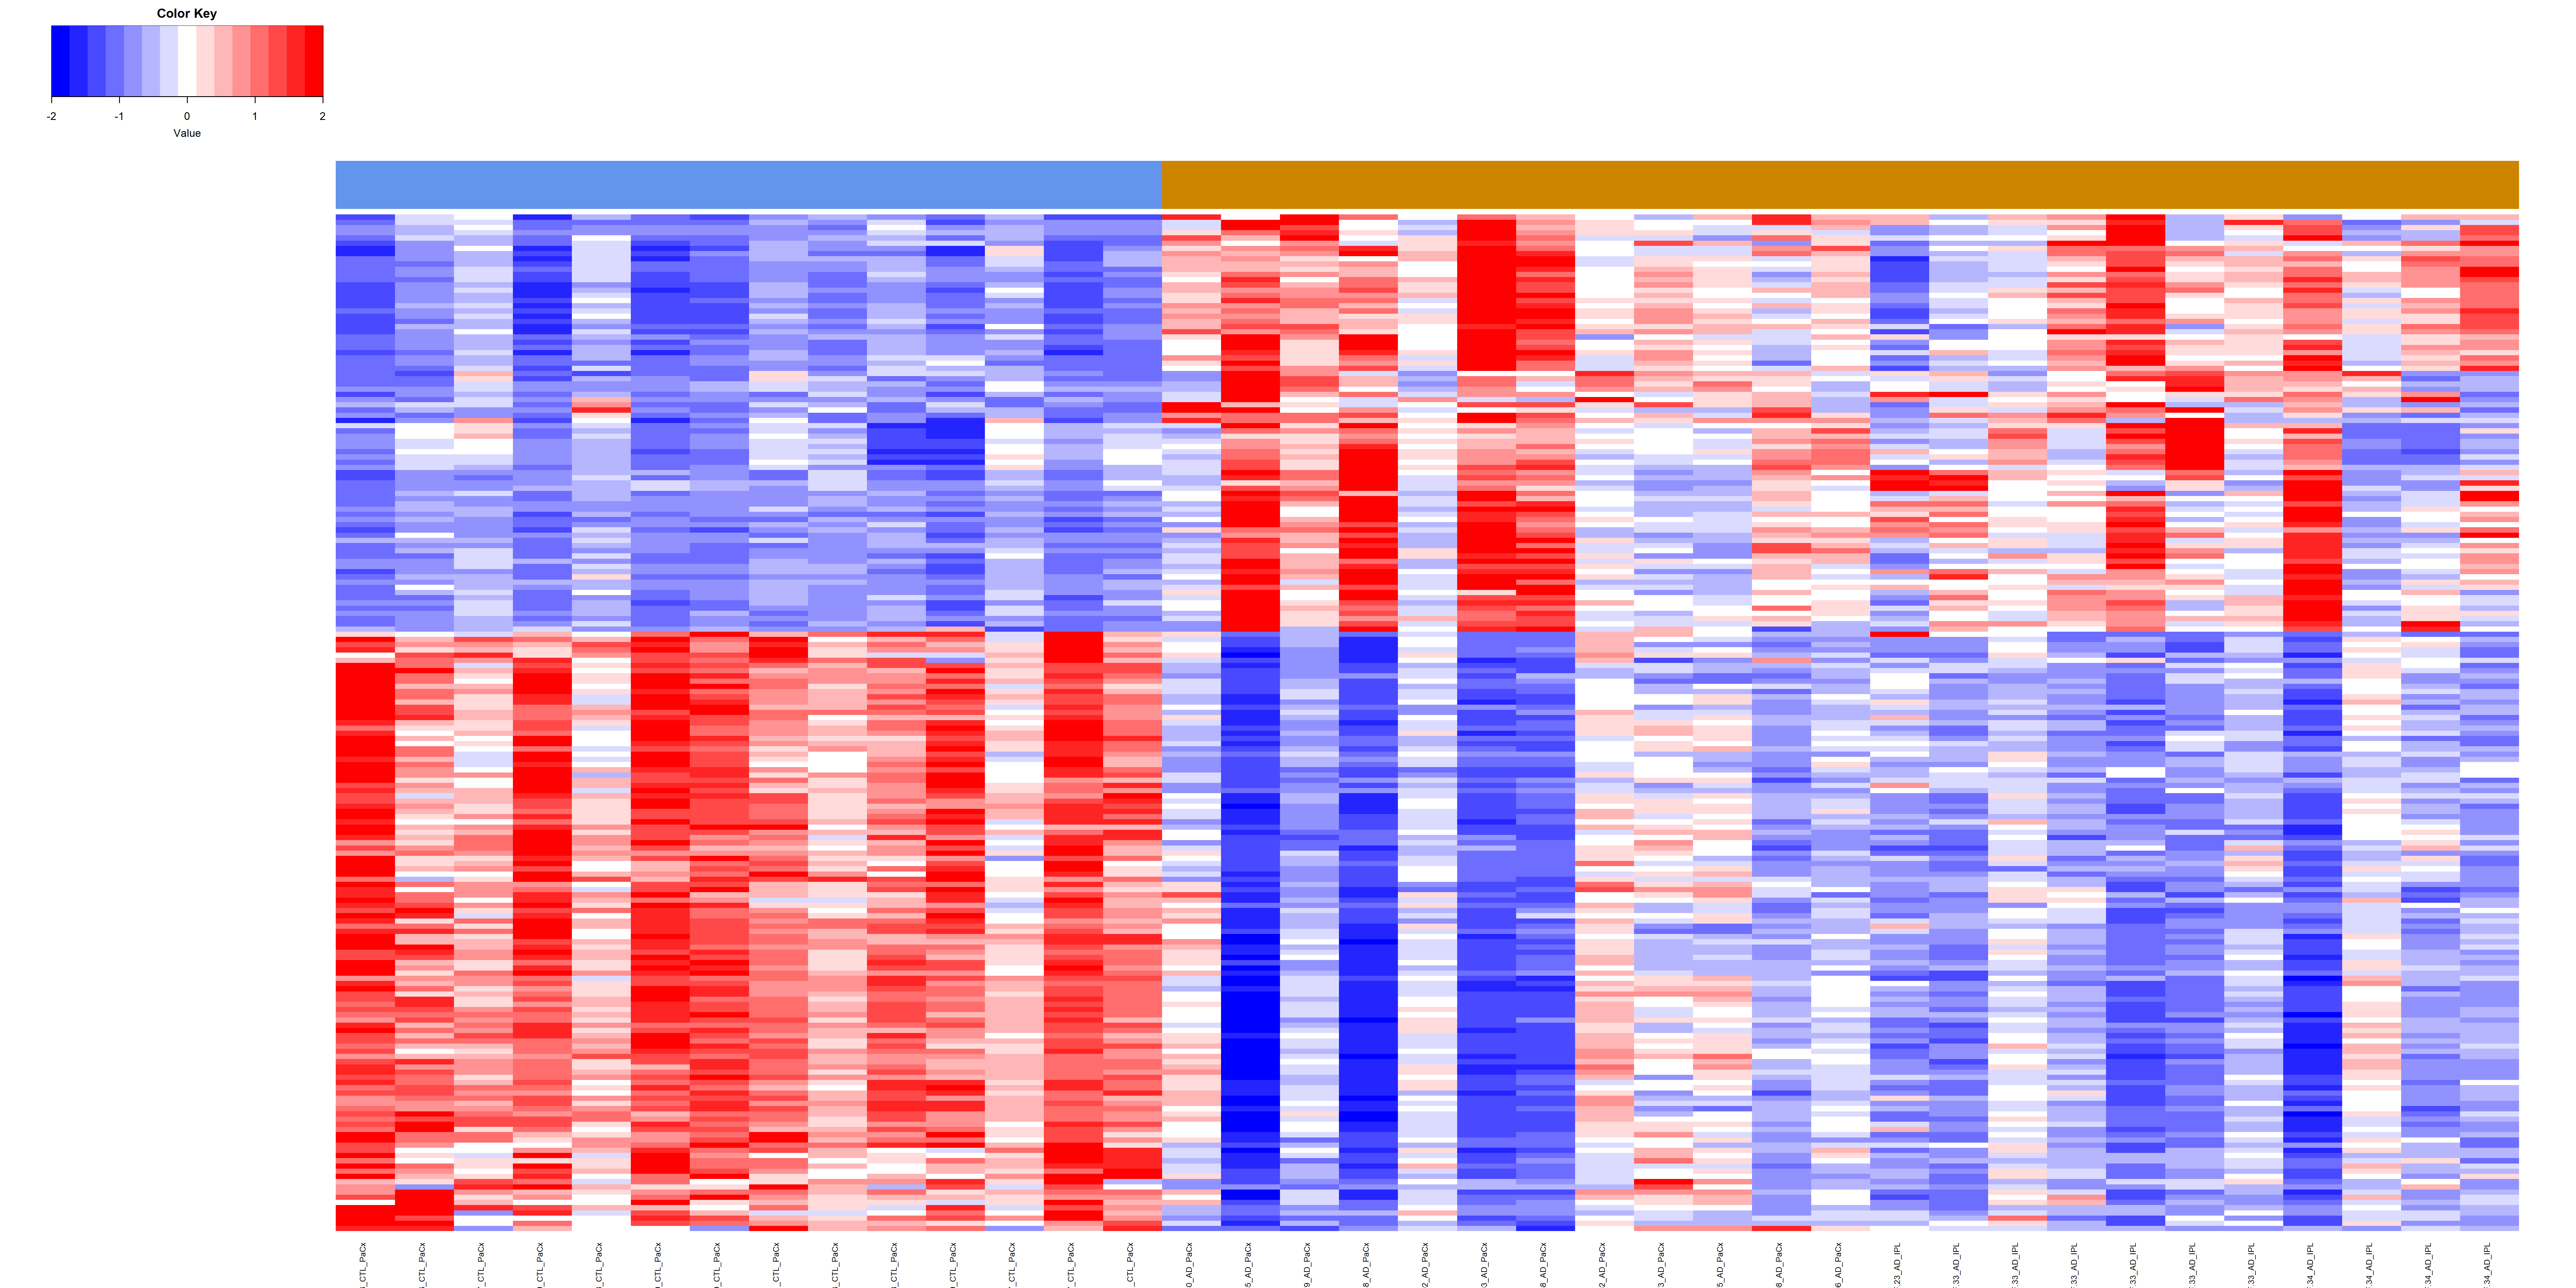
\includegraphics[width = 11cm]{Figures/DE heatmap/CTLvsAD-Pa-f_all.png}}
\caption{Heatmap of Pa-AD-f dataset for all the differentially expressed genes.}
\label{DE-pa-ad-f}
\footnotesize $|$LFC$| >$ 1; AD is the contrast reference. Blue bar: control samples; golden bar: AD samples.
\end{figure}

%\section{Heatmaps for Pa-AD-m comparisons} 

\begin{figure}[!ht]
    \centerline{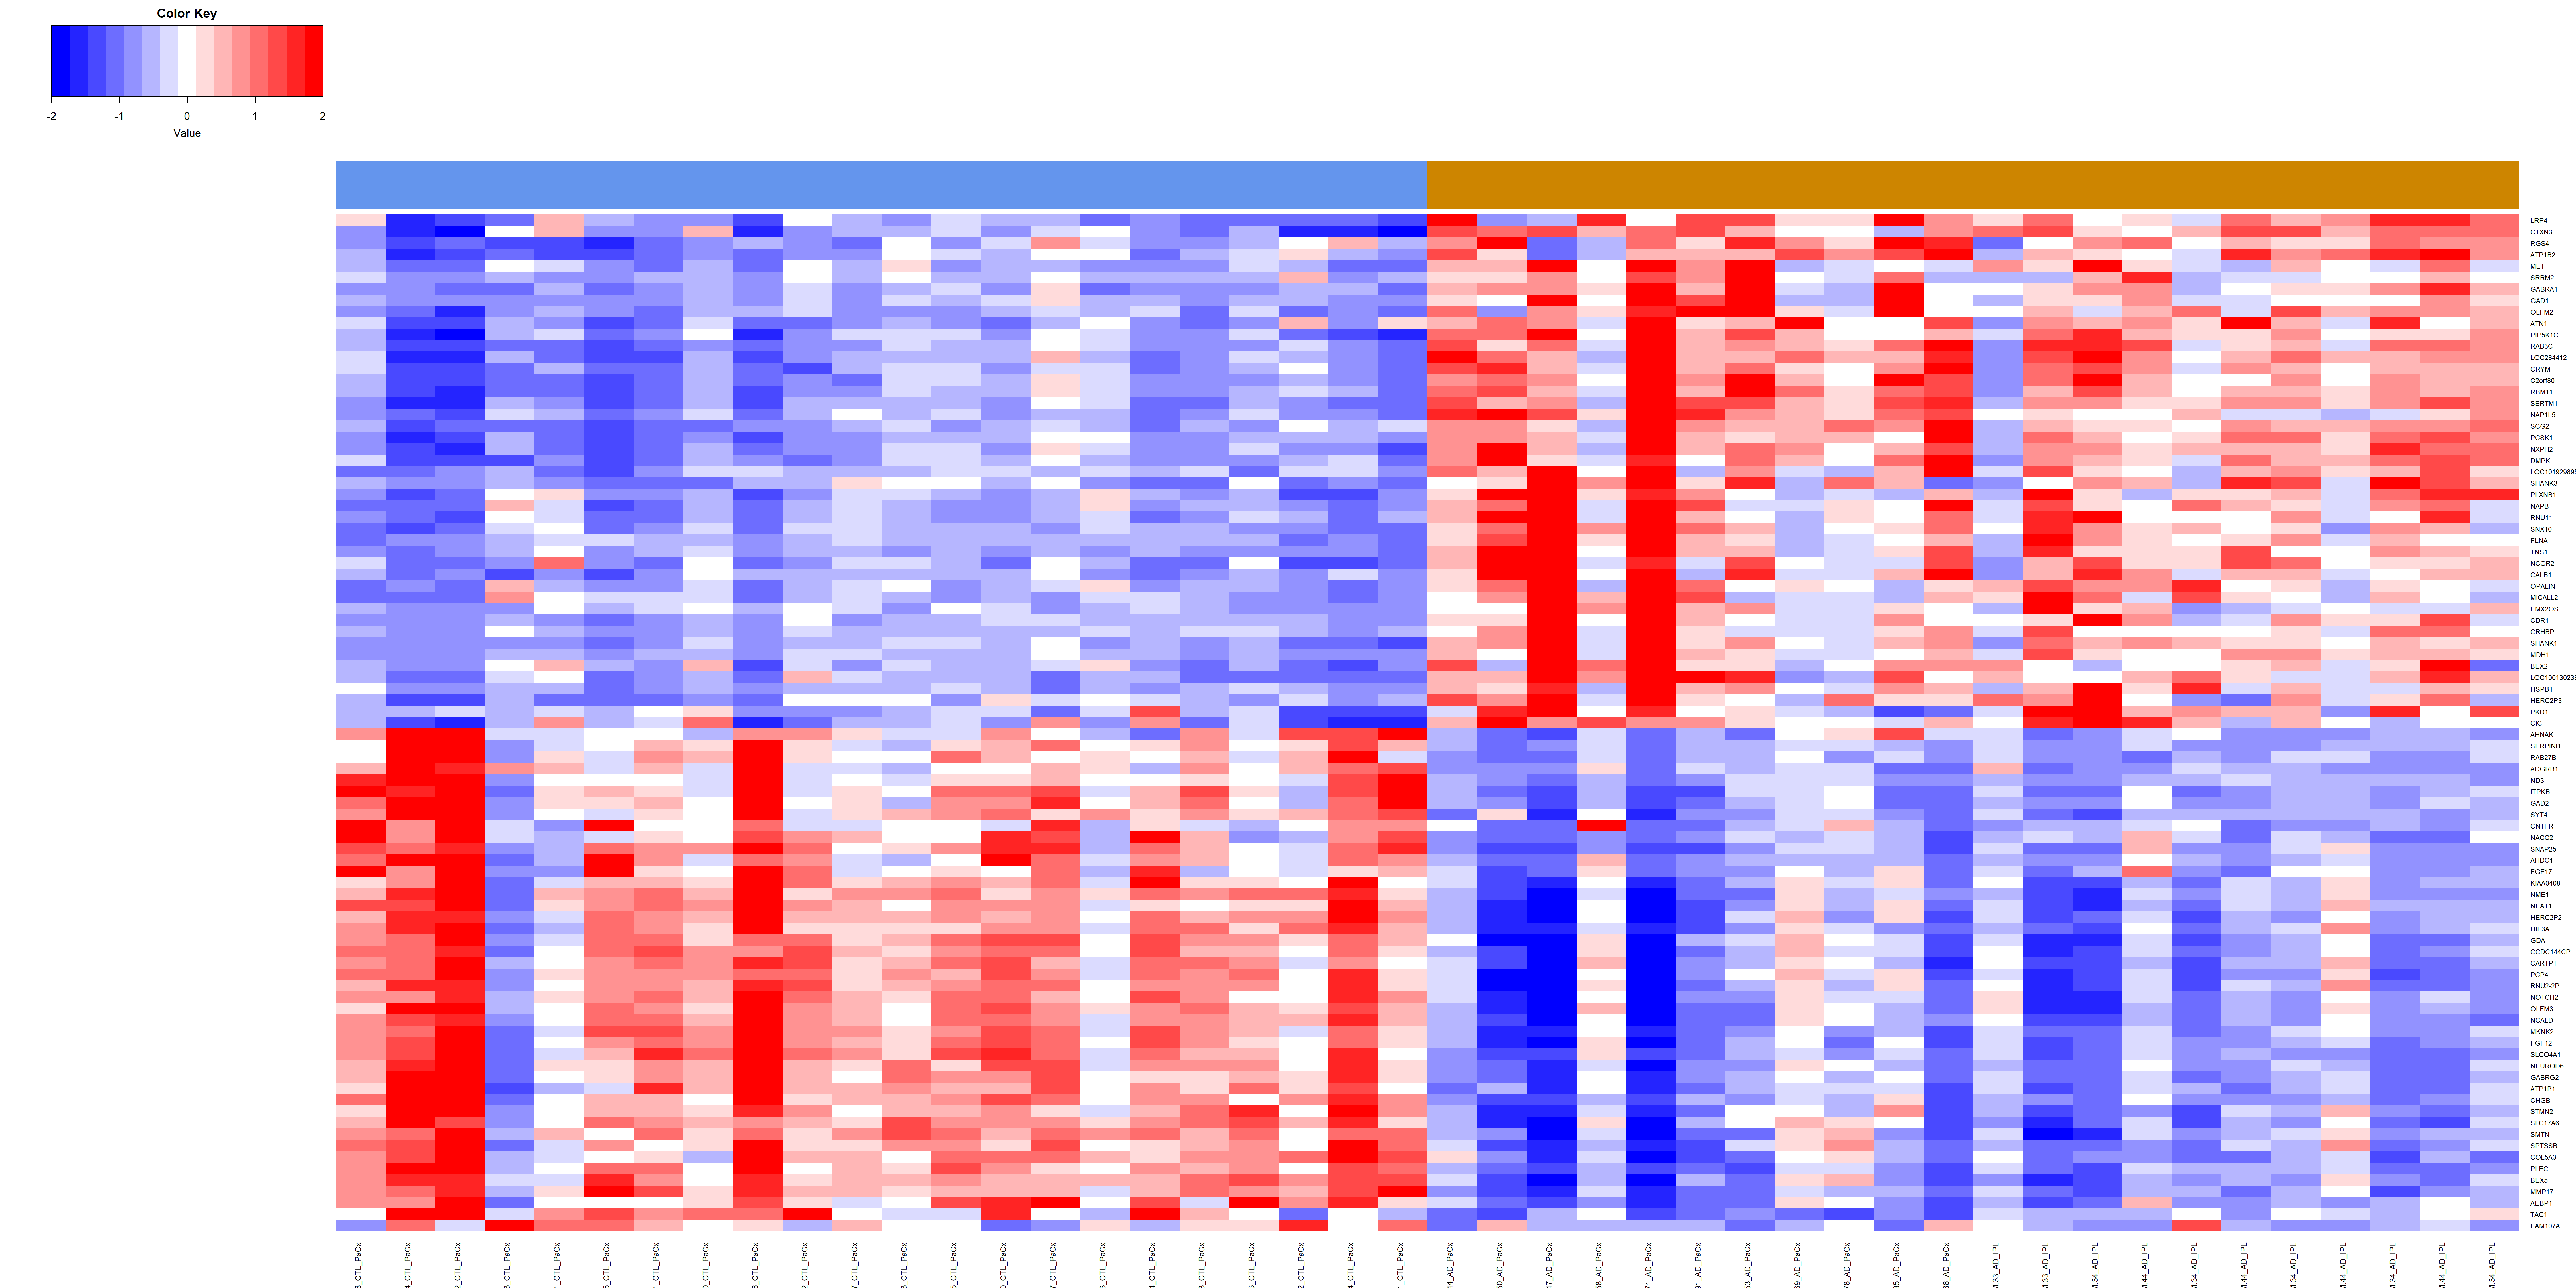
\includegraphics[width = 11cm]{Figures/DE heatmap/CTLvsAD-Pa-m_89.png}}
\caption{Heatmap of Pa-AD-m dataset for all the differentially expressed genes (89 genes).}
\label{DE-pa-ad-m}
\footnotesize $|$LFC$| >$ 1; AD is the contrast reference. Blue bar: control samples; golden bar: AD samples.
\end{figure}

%\section{Heatmaps for Temp-AD-f comparisons} 

\begin{figure}[!ht]
    \centerline{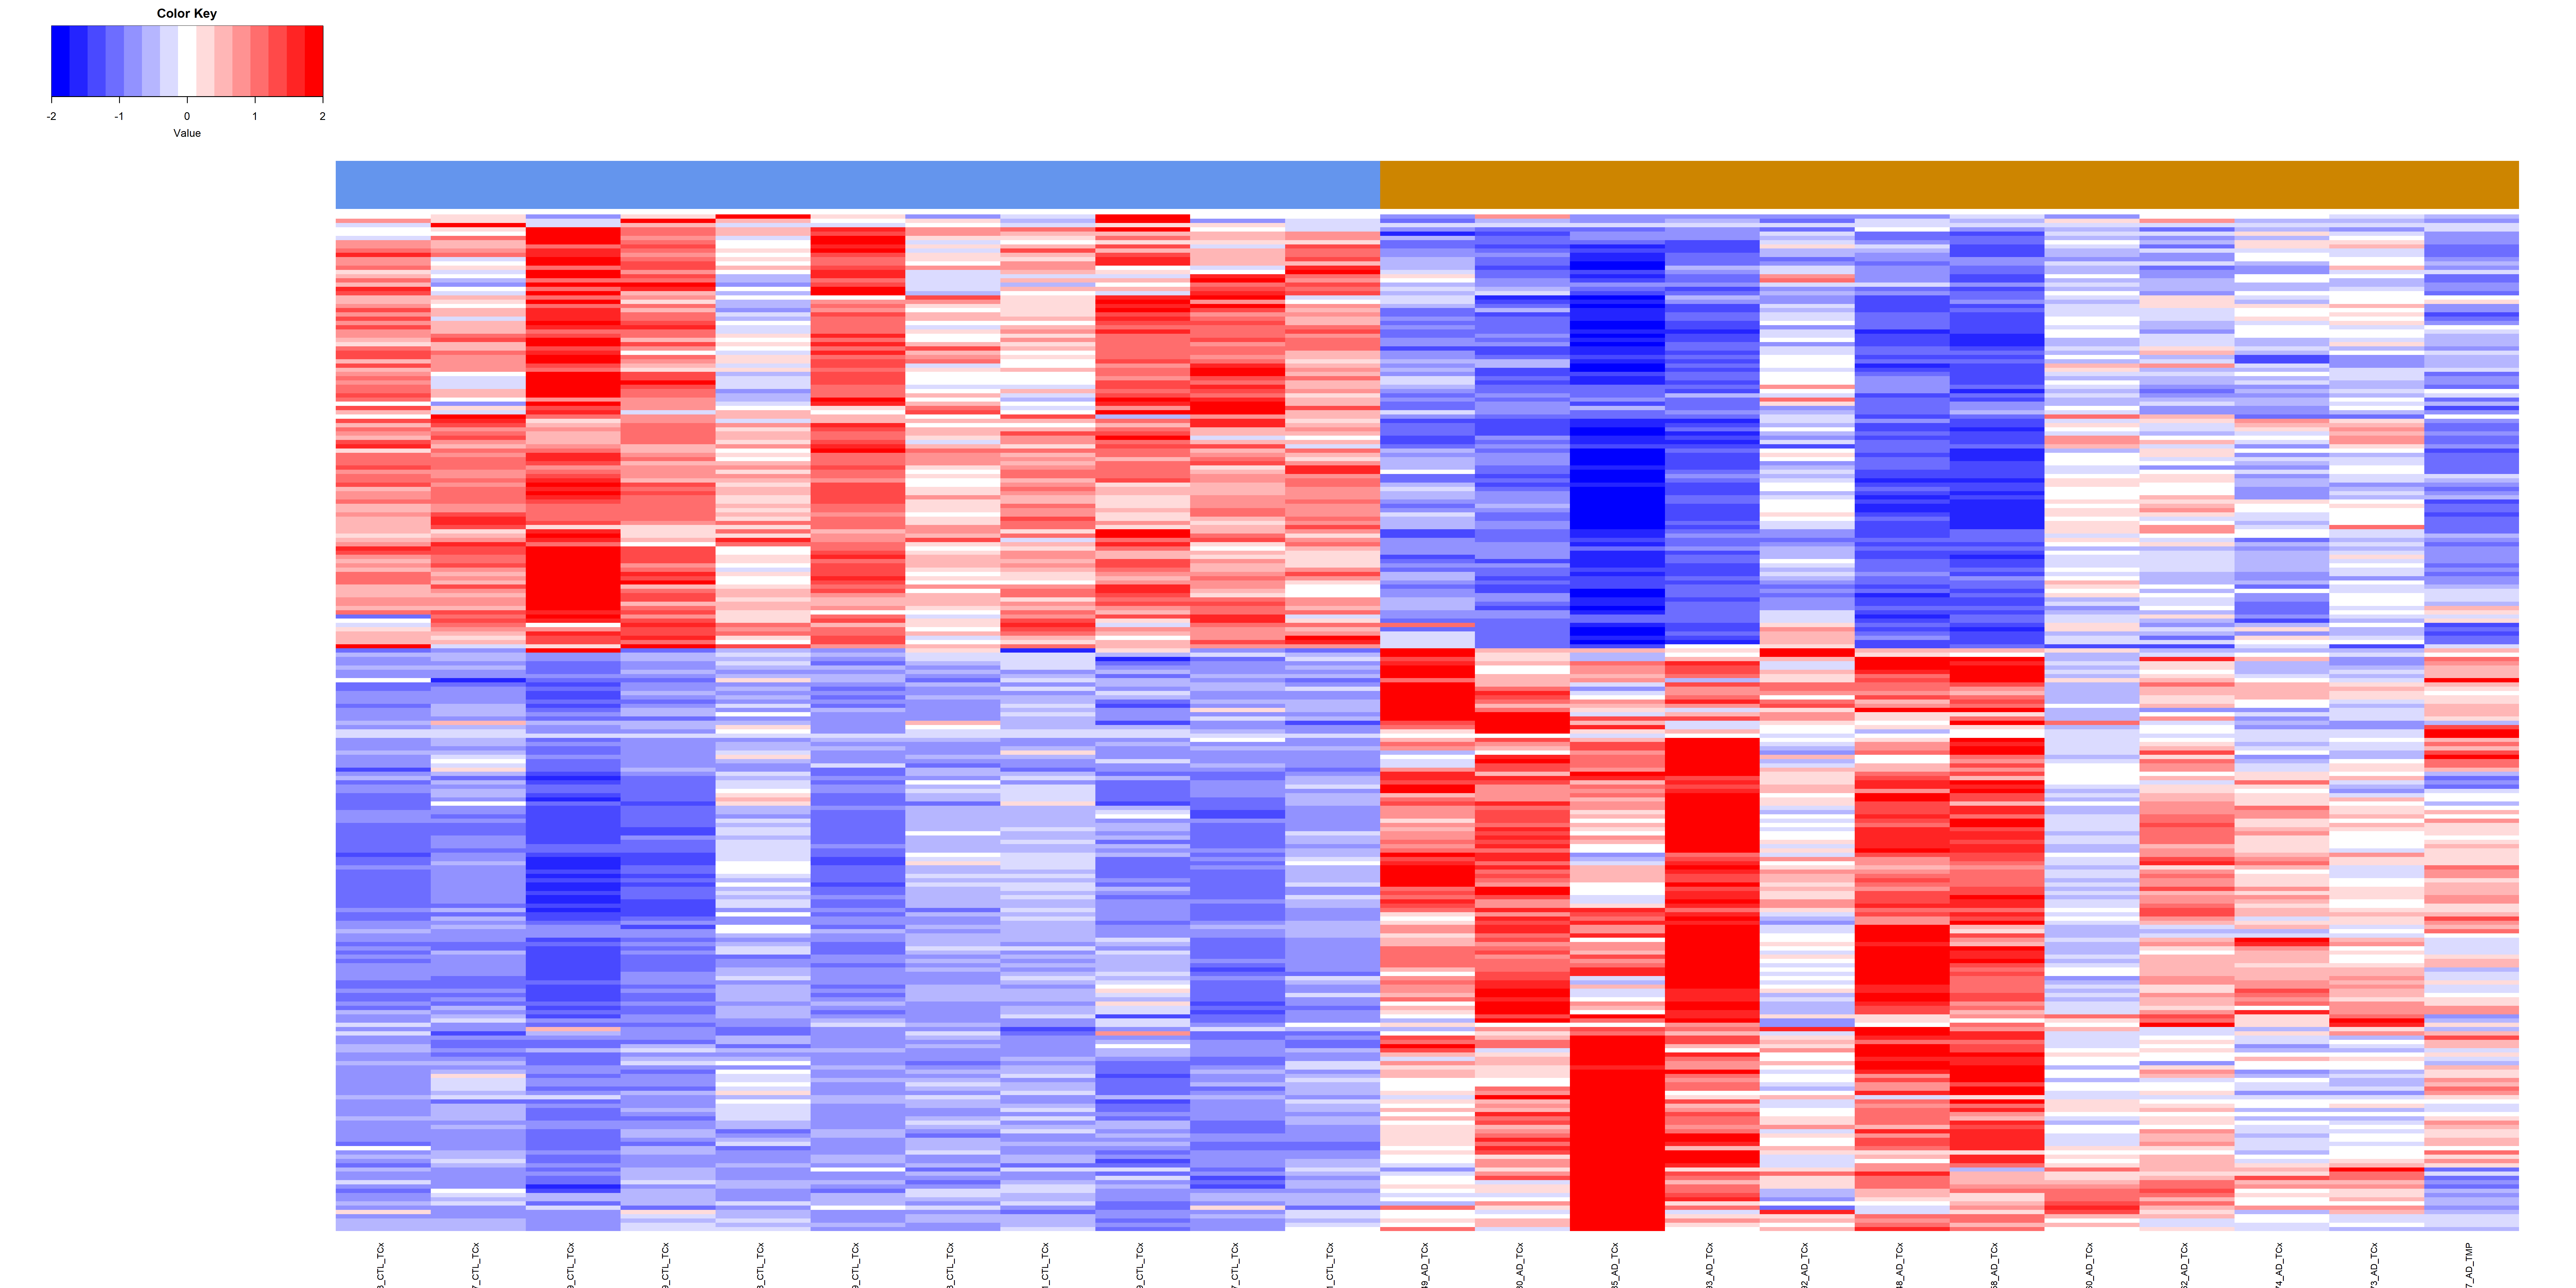
\includegraphics[width = 11cm]{Figures/DE heatmap/CTLvsAD-TCx-f_all.png}}
\caption{Heatmap of Temp-AD-f dataset for all the differentially expressed genes.}
\label{DE-temp-ad-f}
\footnotesize $|$LFC$| >$ 1; AD is the contrast reference. Blue bar: control samples; golden bar: AD samples.
\end{figure}

%\section{Heatmaps for Temp-AD-m comparisons}

\begin{figure}[!ht]
    \centerline{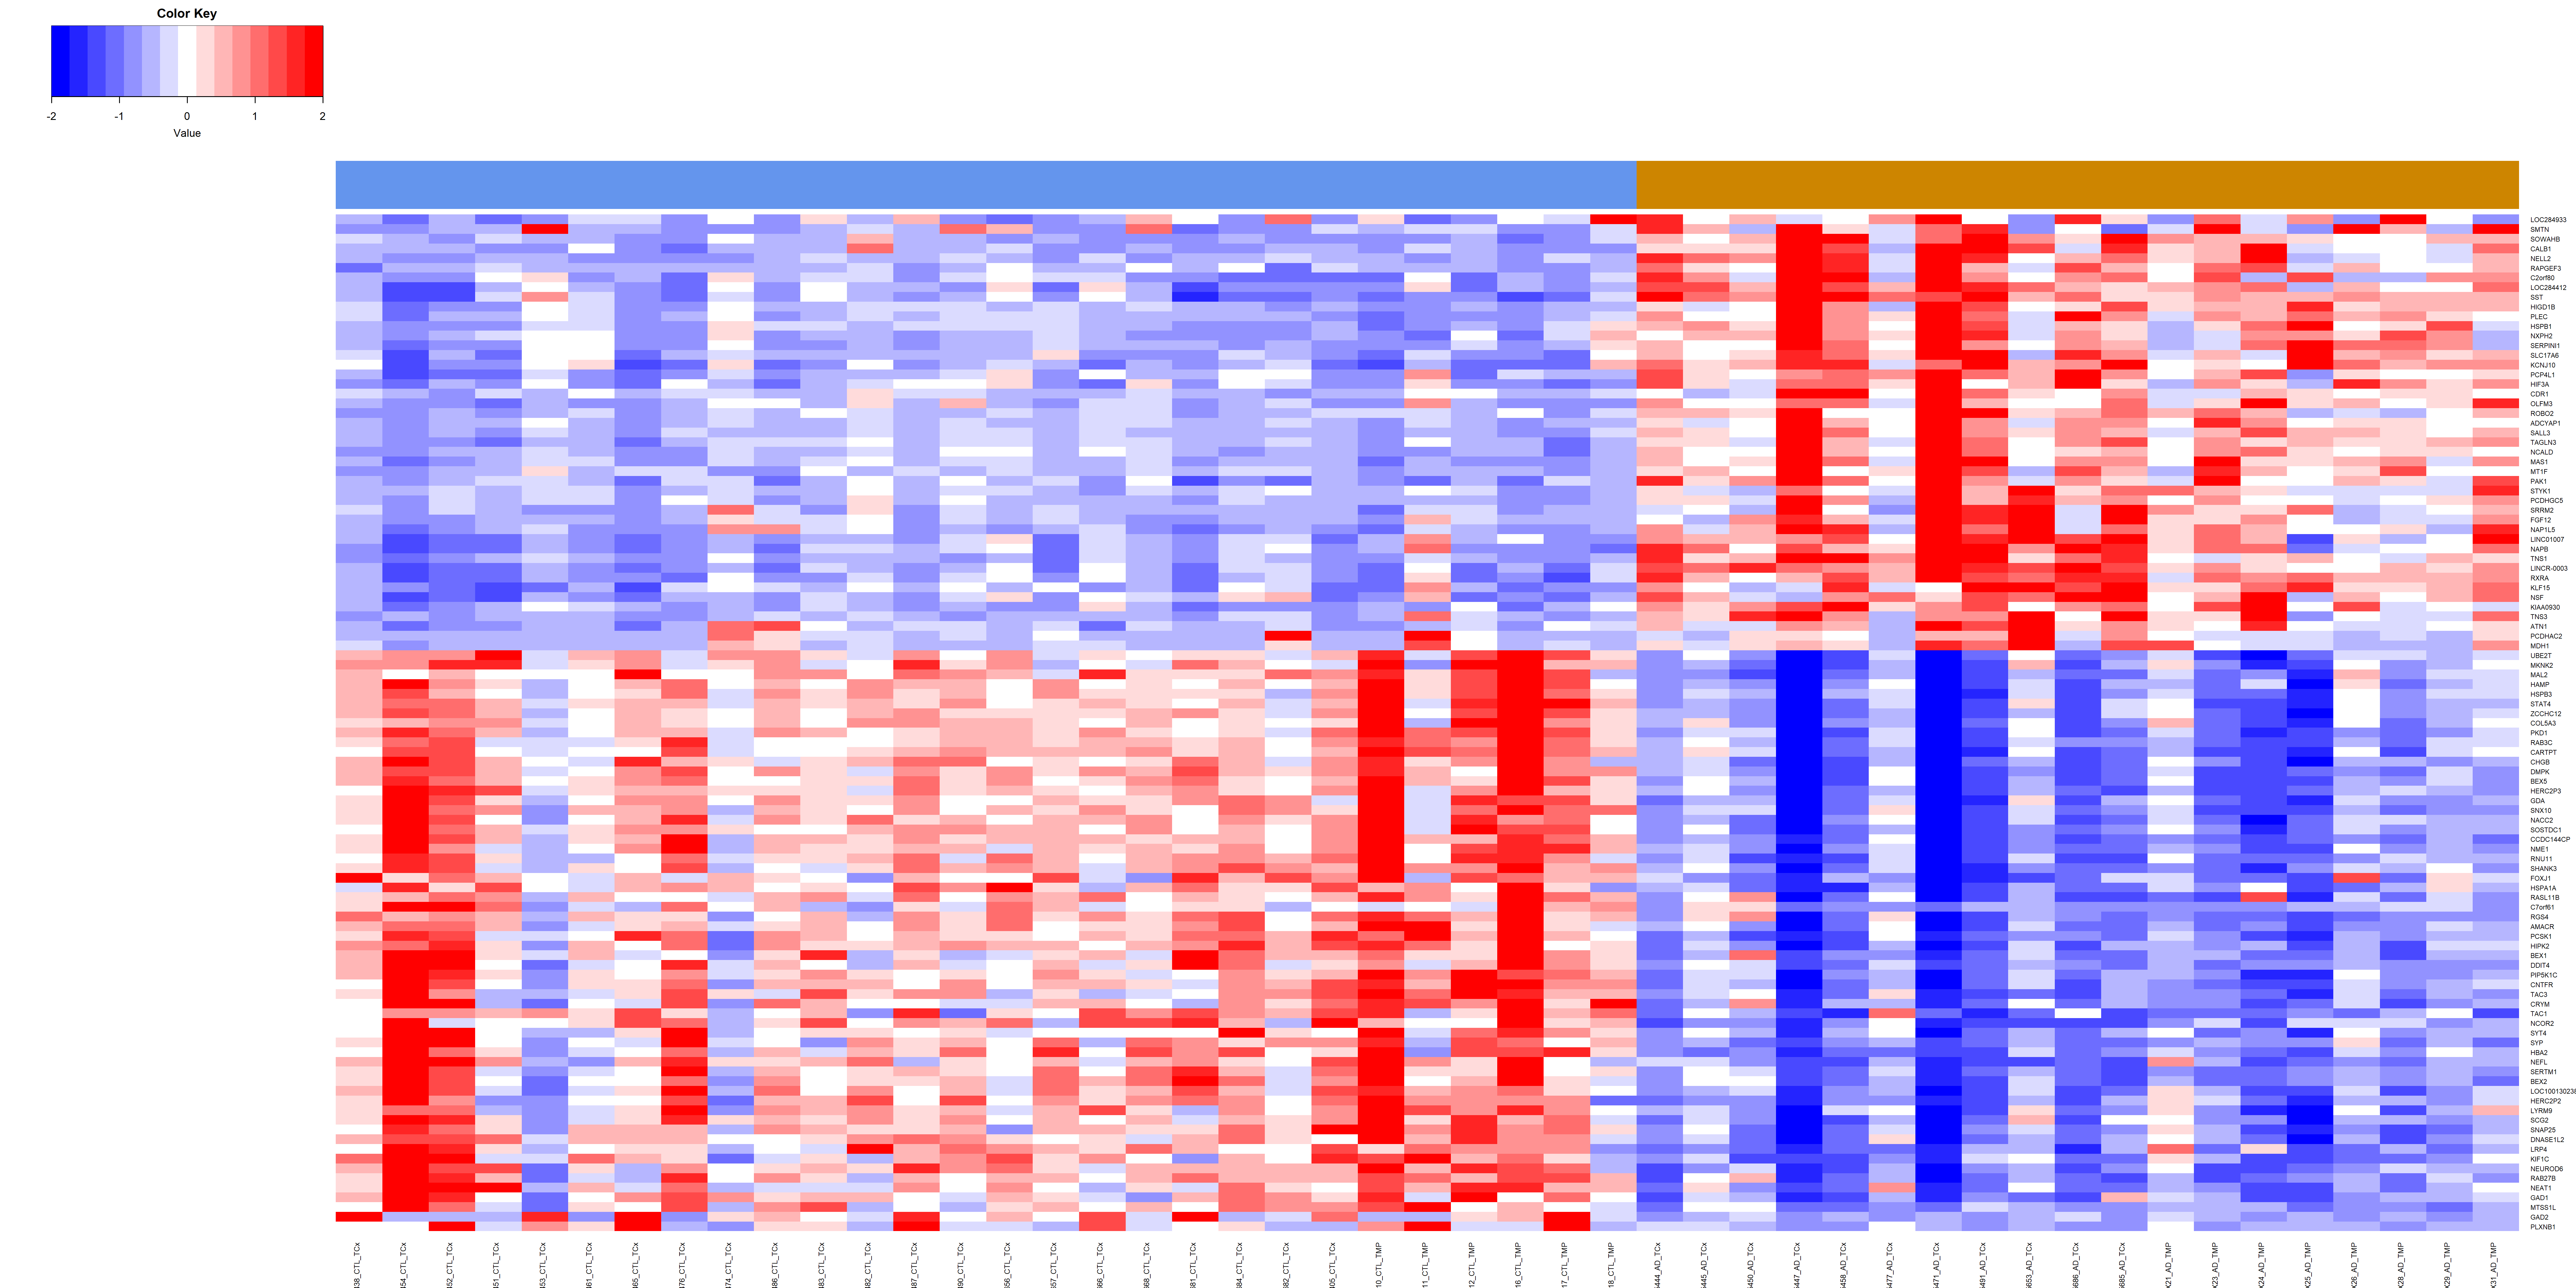
\includegraphics[width = 11cm]{Figures/DE heatmap/CTLvsAD-TCx-m_105.png}}
\caption{Heatmap of Temp-AD-m dataset for all the differentially expressed genes (105 genes).}
\label{DE-temp-ad-m}
\footnotesize $|$LFC$| >$ 1; AD is the contrast reference. Blue bar: control samples; golden bar: AD samples.
\end{figure}

%\section{Heatmaps for Hip-AD-f comparisons} 

\begin{figure}[!ht]
    \centerline{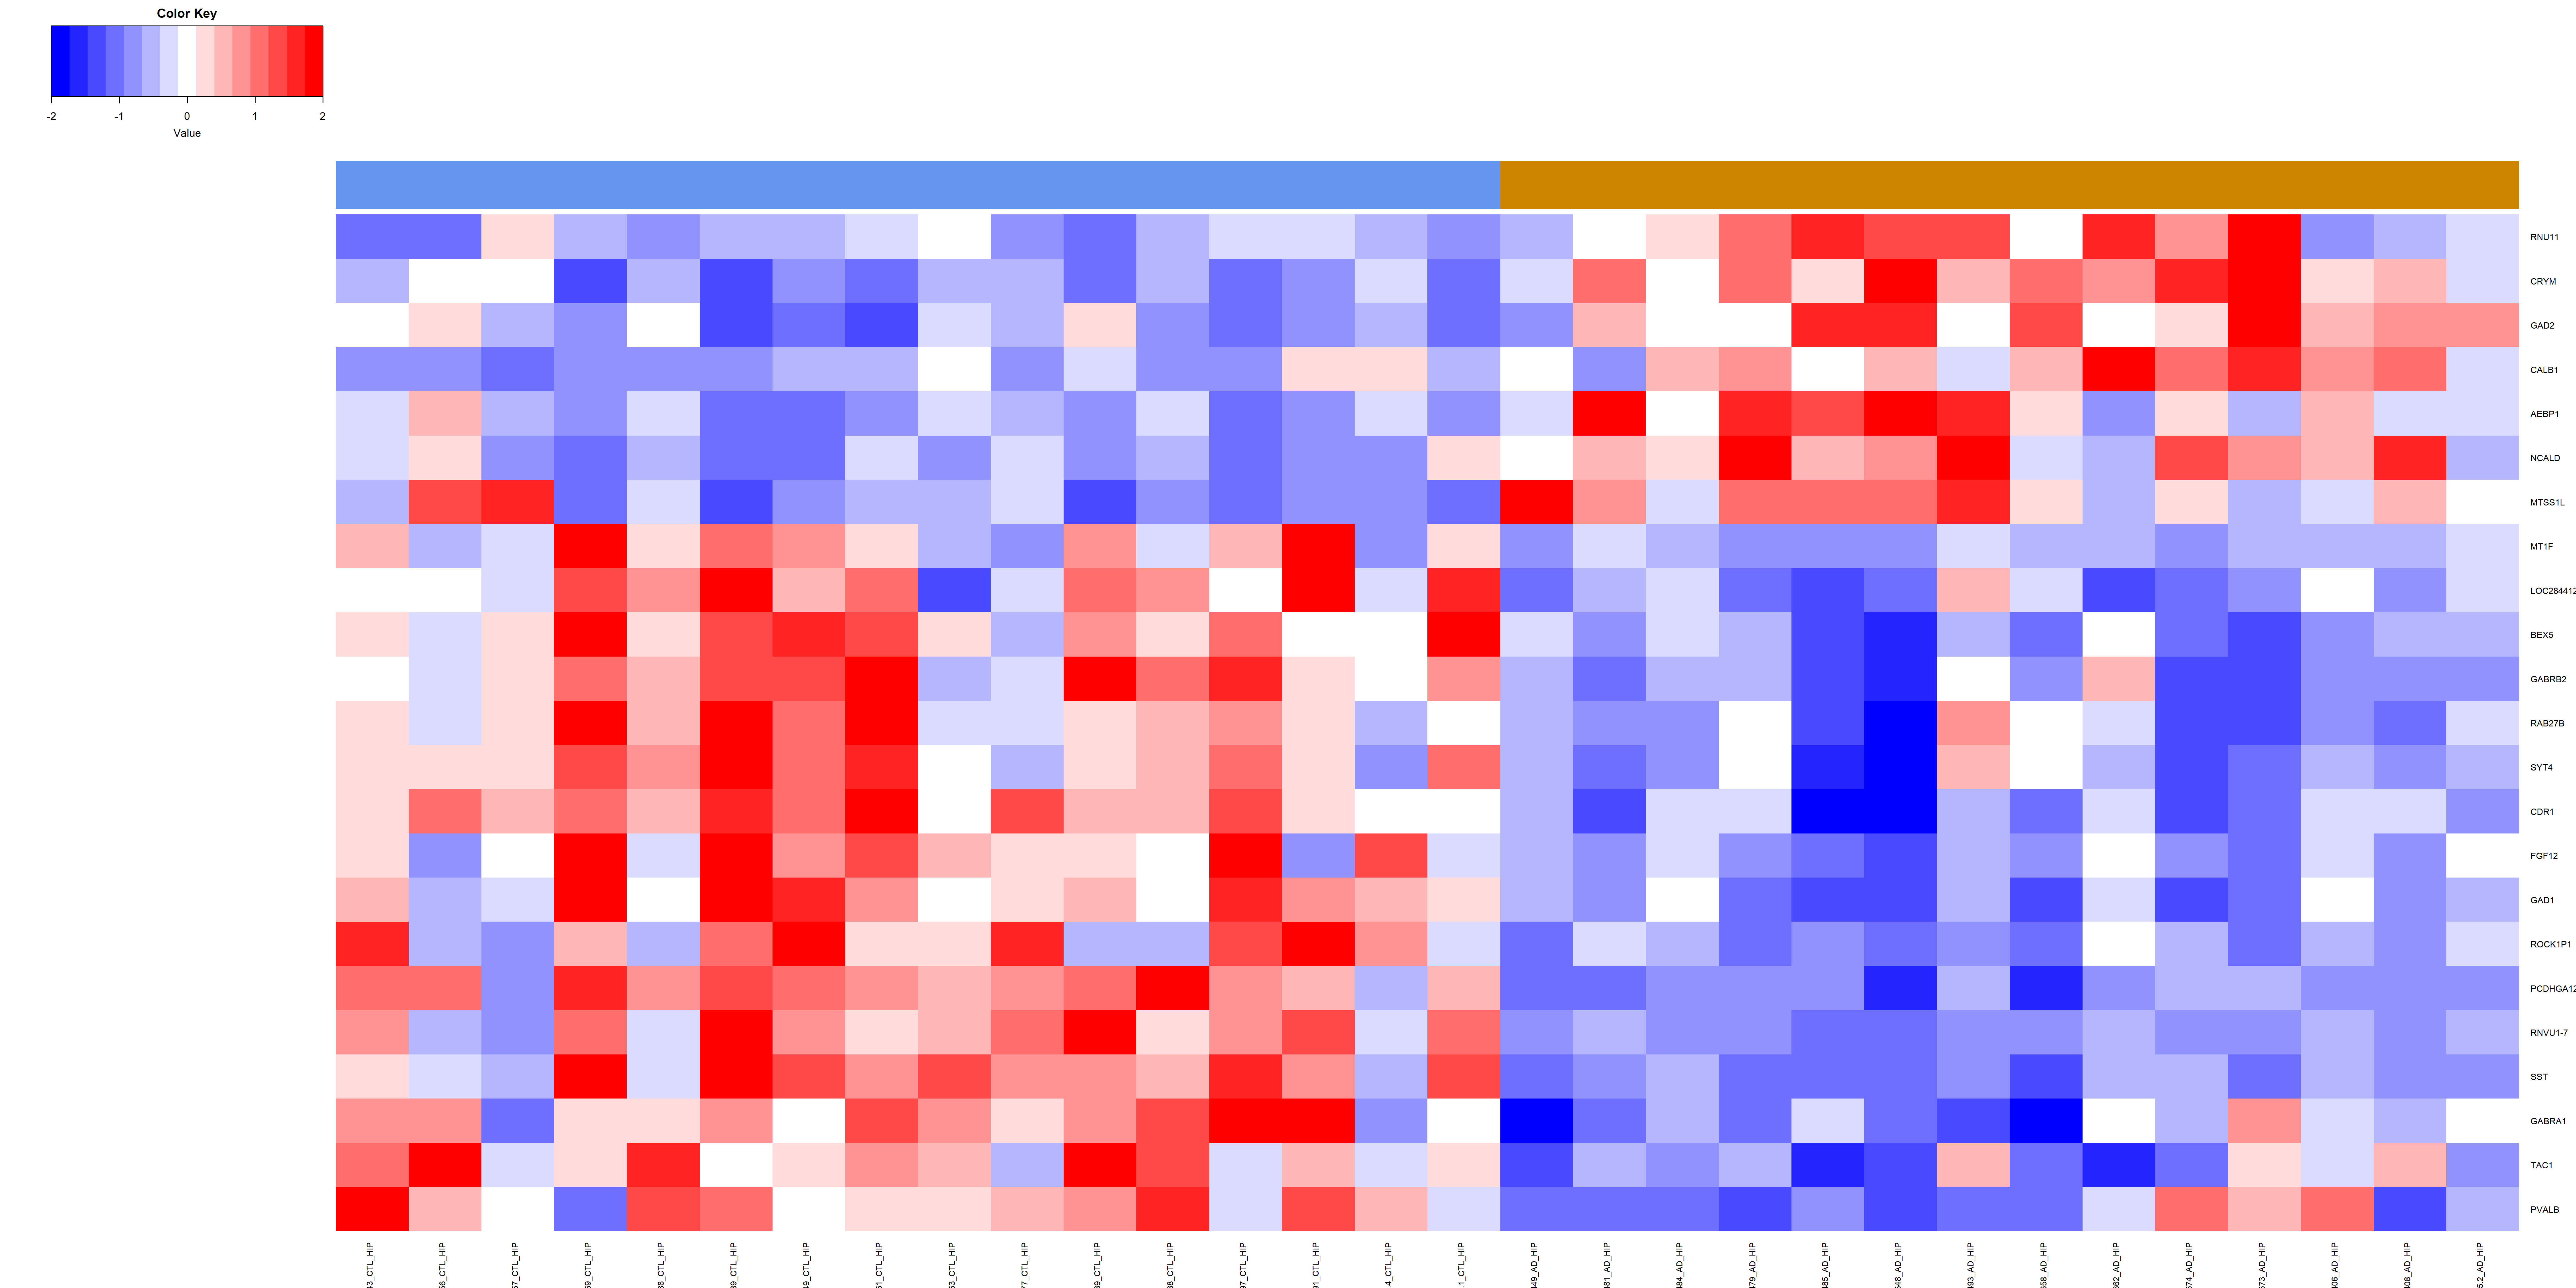
\includegraphics[width = 11cm]{Figures/DE heatmap/CTLvsAD-HIP-f_23.png}}
\caption{Heatmap of Hip-AD-f dataset for all the differentially expressed genes (23 genes).}
\label{DE-hip-ad-f}
\footnotesize $|$LFC$| >$ 1; AD is the contrast reference. Blue bar: control samples; golden bar: AD samples.
\end{figure}

%\section{Heatmaps for Hip-AD-m comparisons} 

\begin{figure}[!ht]
    \centerline{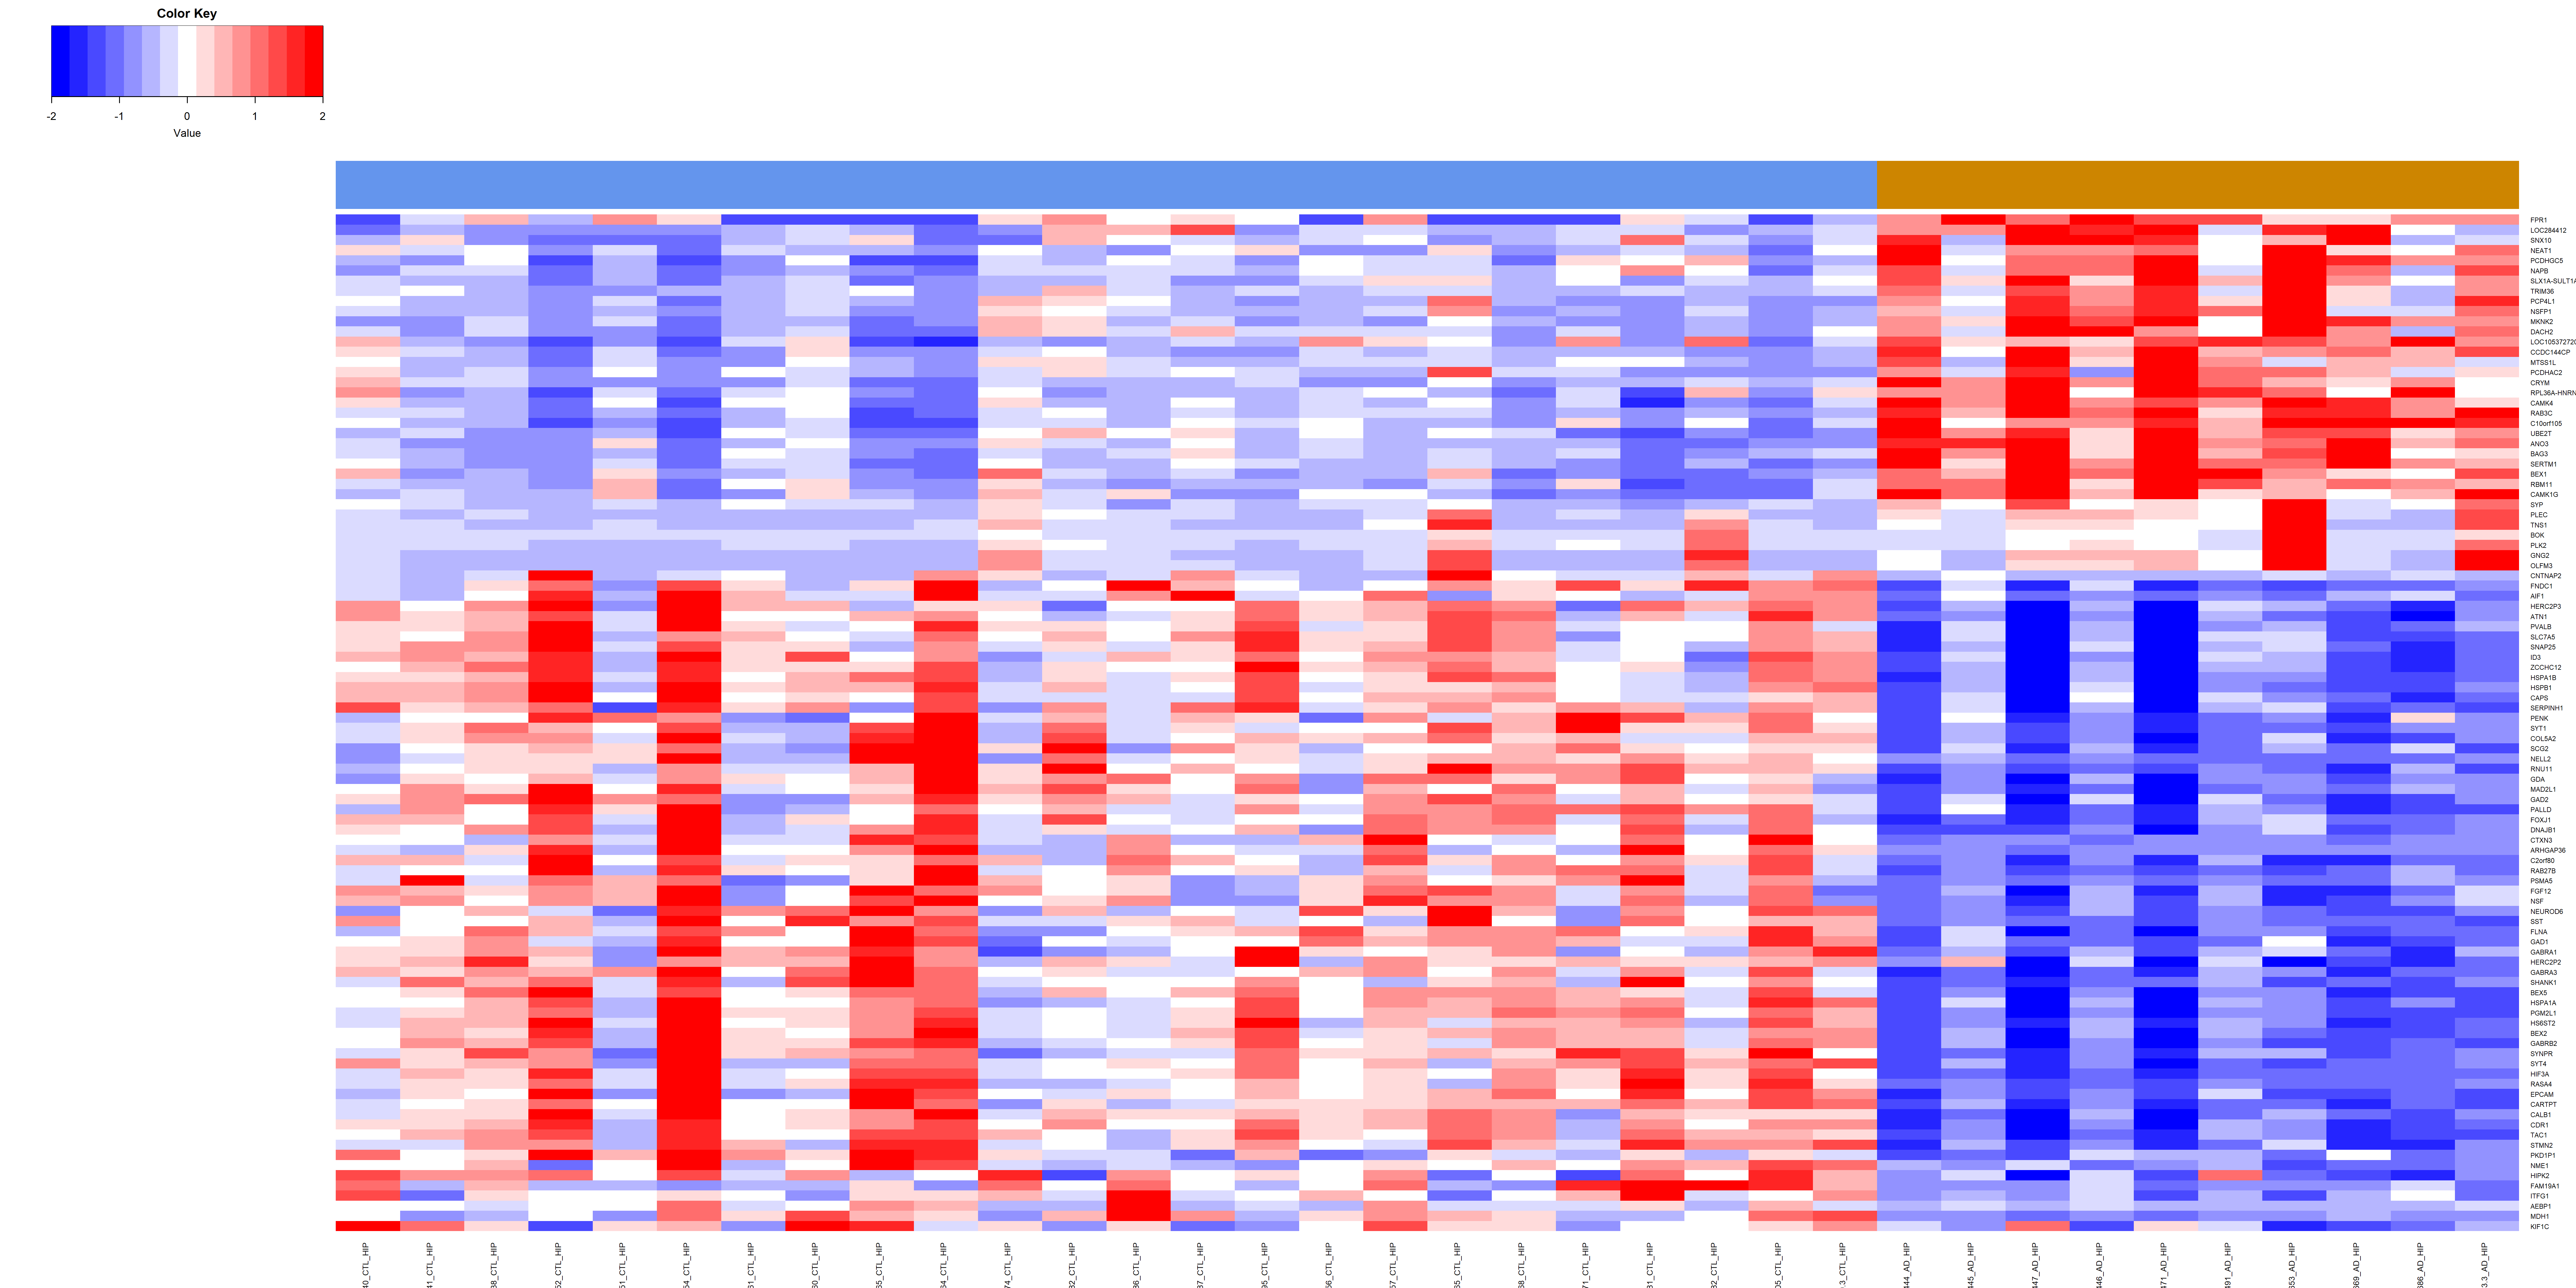
\includegraphics[width = 11cm]{Figures/DE heatmap/CTLvsAD-HIP-m_100.png}}
\caption{Heatmap of Hip-AD-m dataset for all the differentially expressed genes (100 genes).}
\label{DE-hip-ad-m}
\footnotesize $|$LFC$| >$ 1; AD is the contrast reference. Blue bar: control samples; golden bar: AD samples.
\end{figure}

%\section{Heatmaps for Front-AD-f comparisons} 

\begin{figure}[!ht]
    \centerline{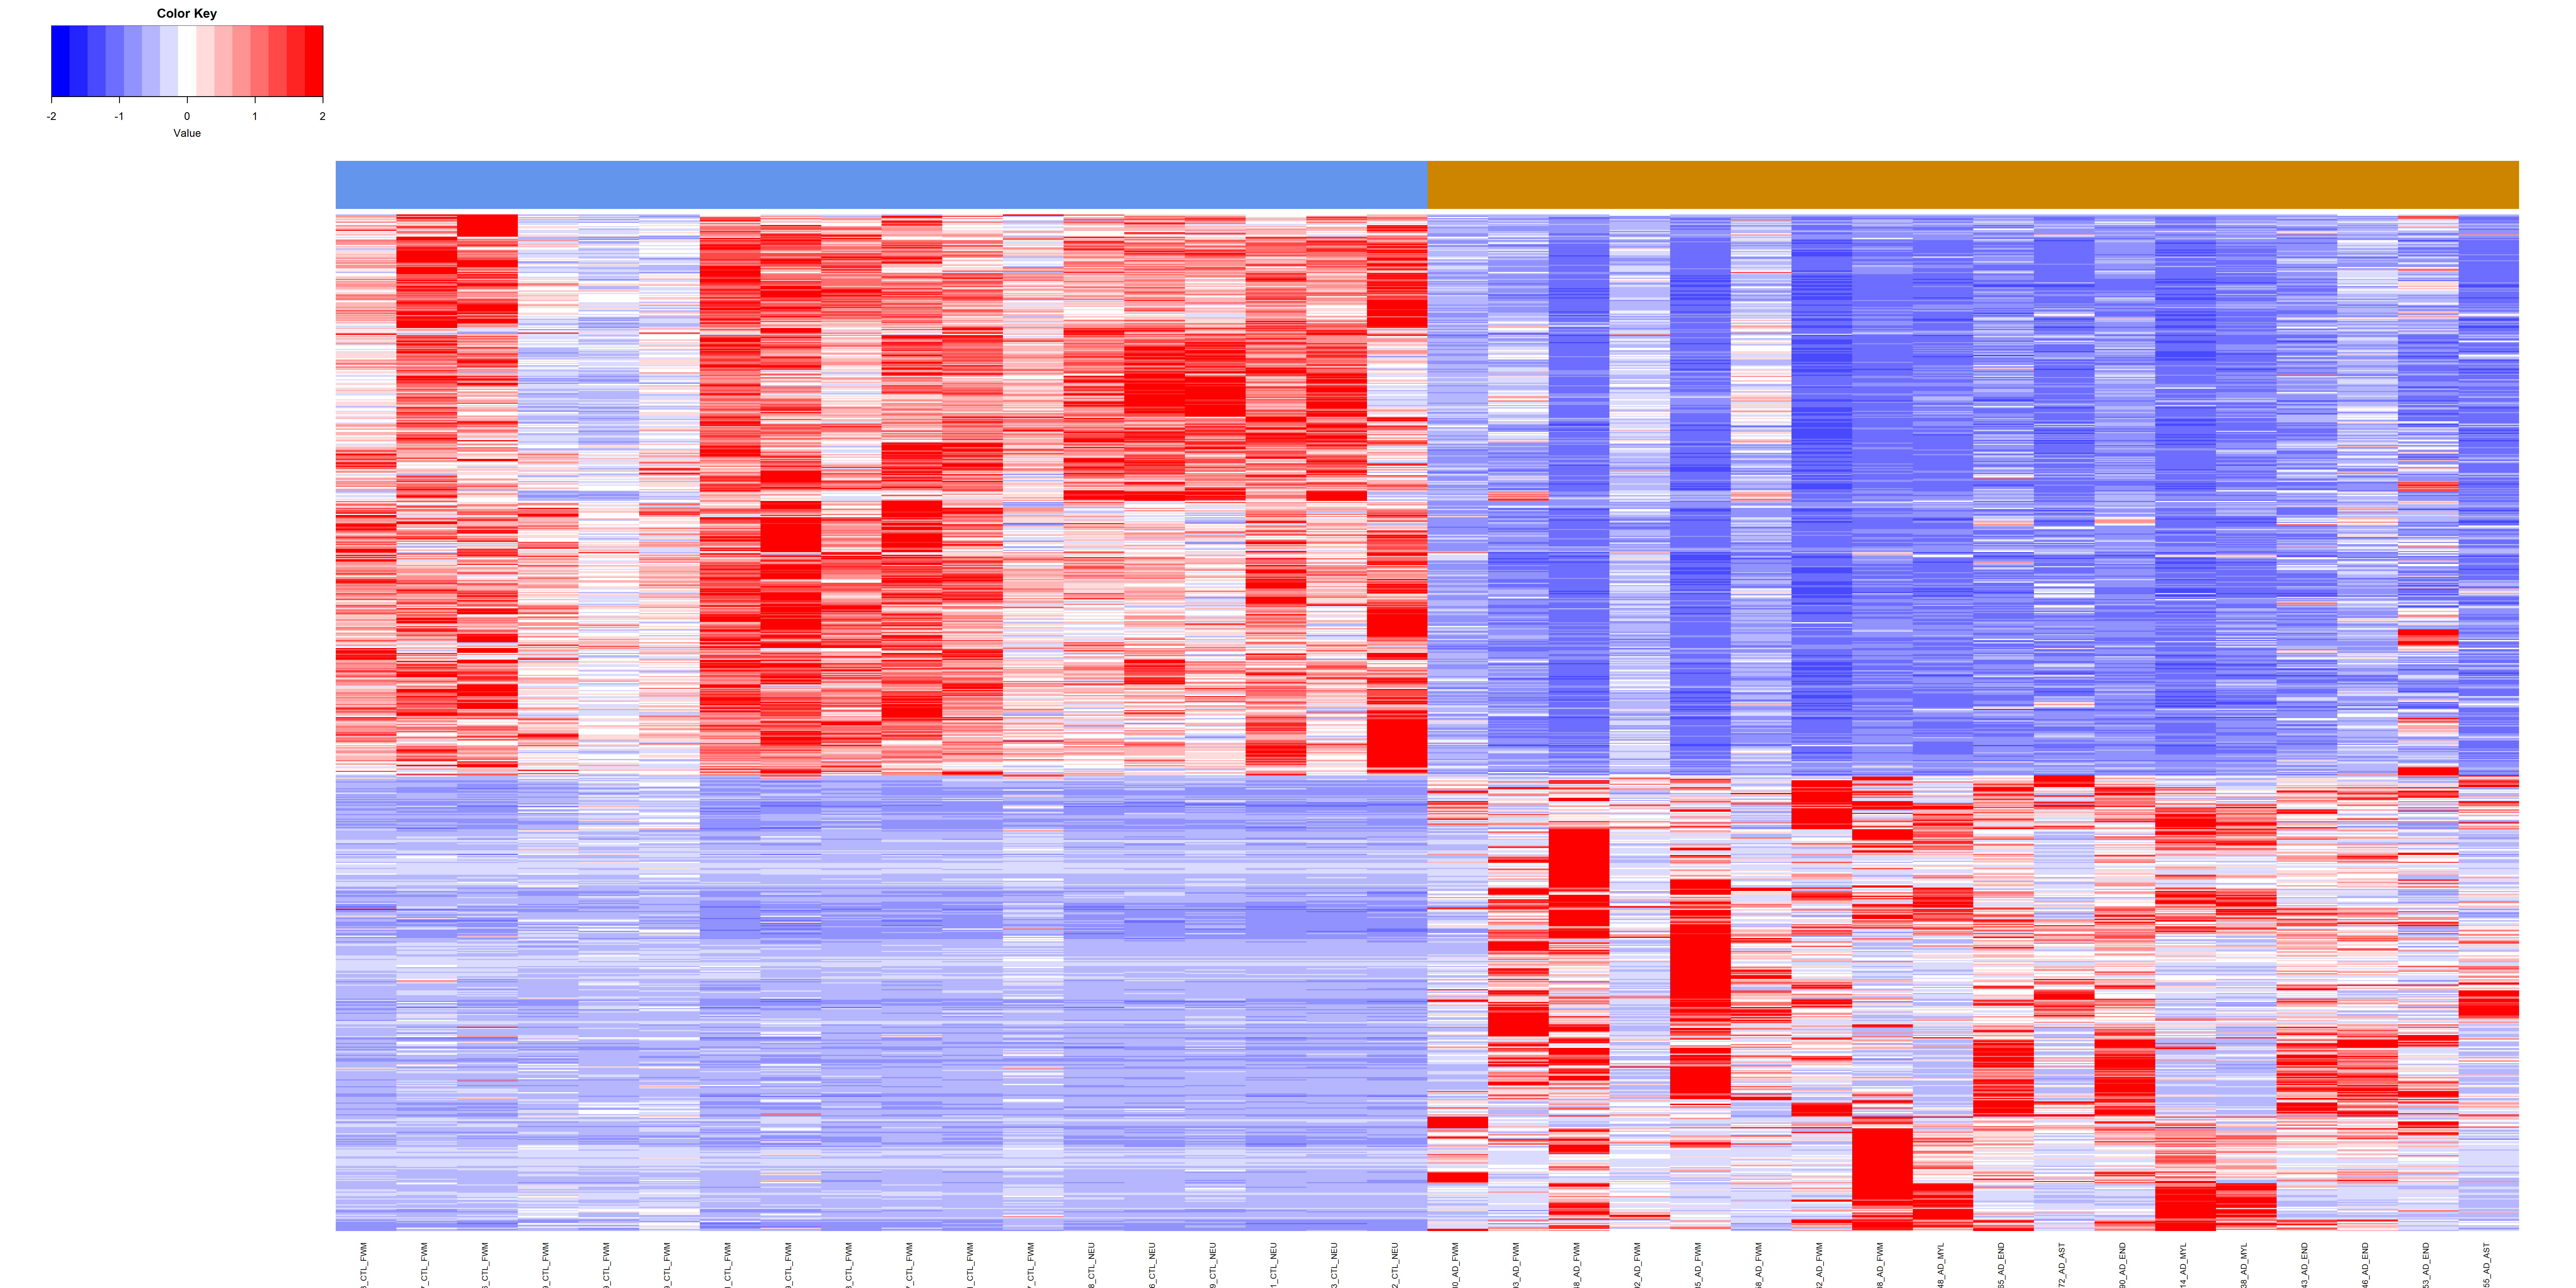
\includegraphics[width = 11cm]{Figures/DE heatmap/CTLvsAD-Front-f_all.png}}
\caption{Heatmap of Front-AD-f dataset for all the differentially expressed genes.}
\label{DE-front-ad-f}
\footnotesize $|$LFC$| >$ 1; AD is the contrast reference. Blue bar: control samples; golden bar: AD samples.
\end{figure}

%\section{Heatmaps for Front-AD-m comparisons} 

\begin{figure}[!ht]
    \centerline{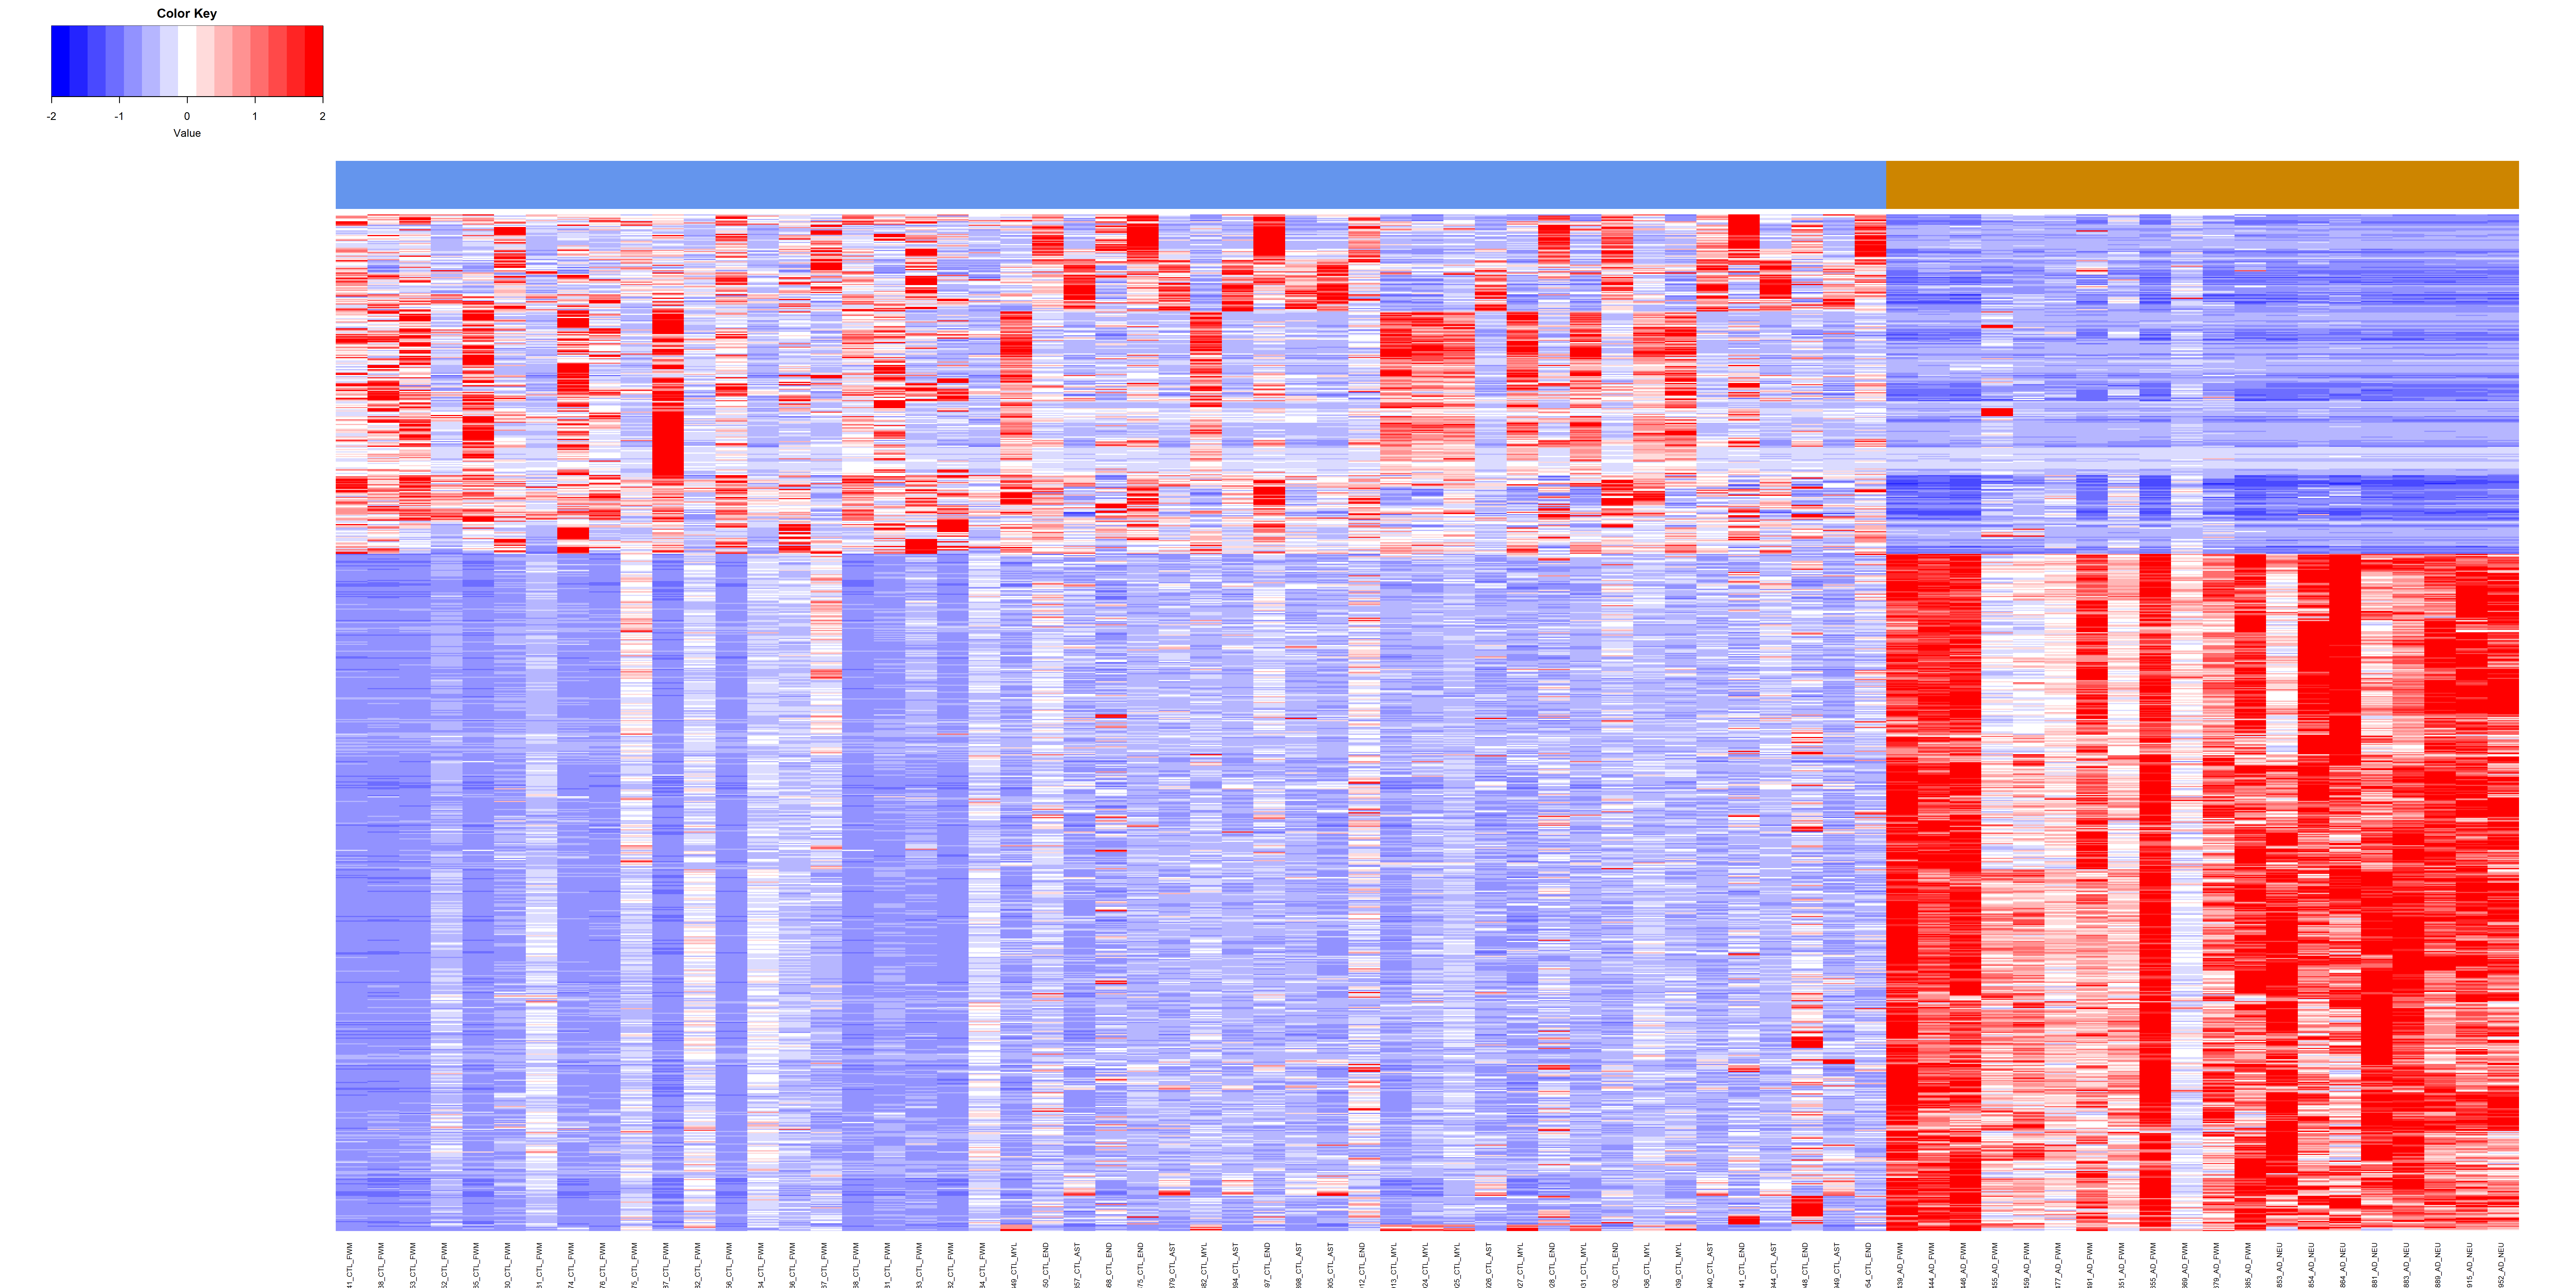
\includegraphics[width = 11cm]{Figures/DE heatmap/CTLvsAD-Front-m_all.png}}
\caption{Heatmap of Front-AD-m dataset for all the differentially expressed genes.}
\label{DE-front-ad-m}
\footnotesize $|$LFC$| >$ 1; AD is the contrast reference. Blue bar: control samples; golden bar: AD samples.
\end{figure}

%\section{Heatmaps for Fus-AD-f comparisons} 

\begin{figure}[!ht]
    \centerline{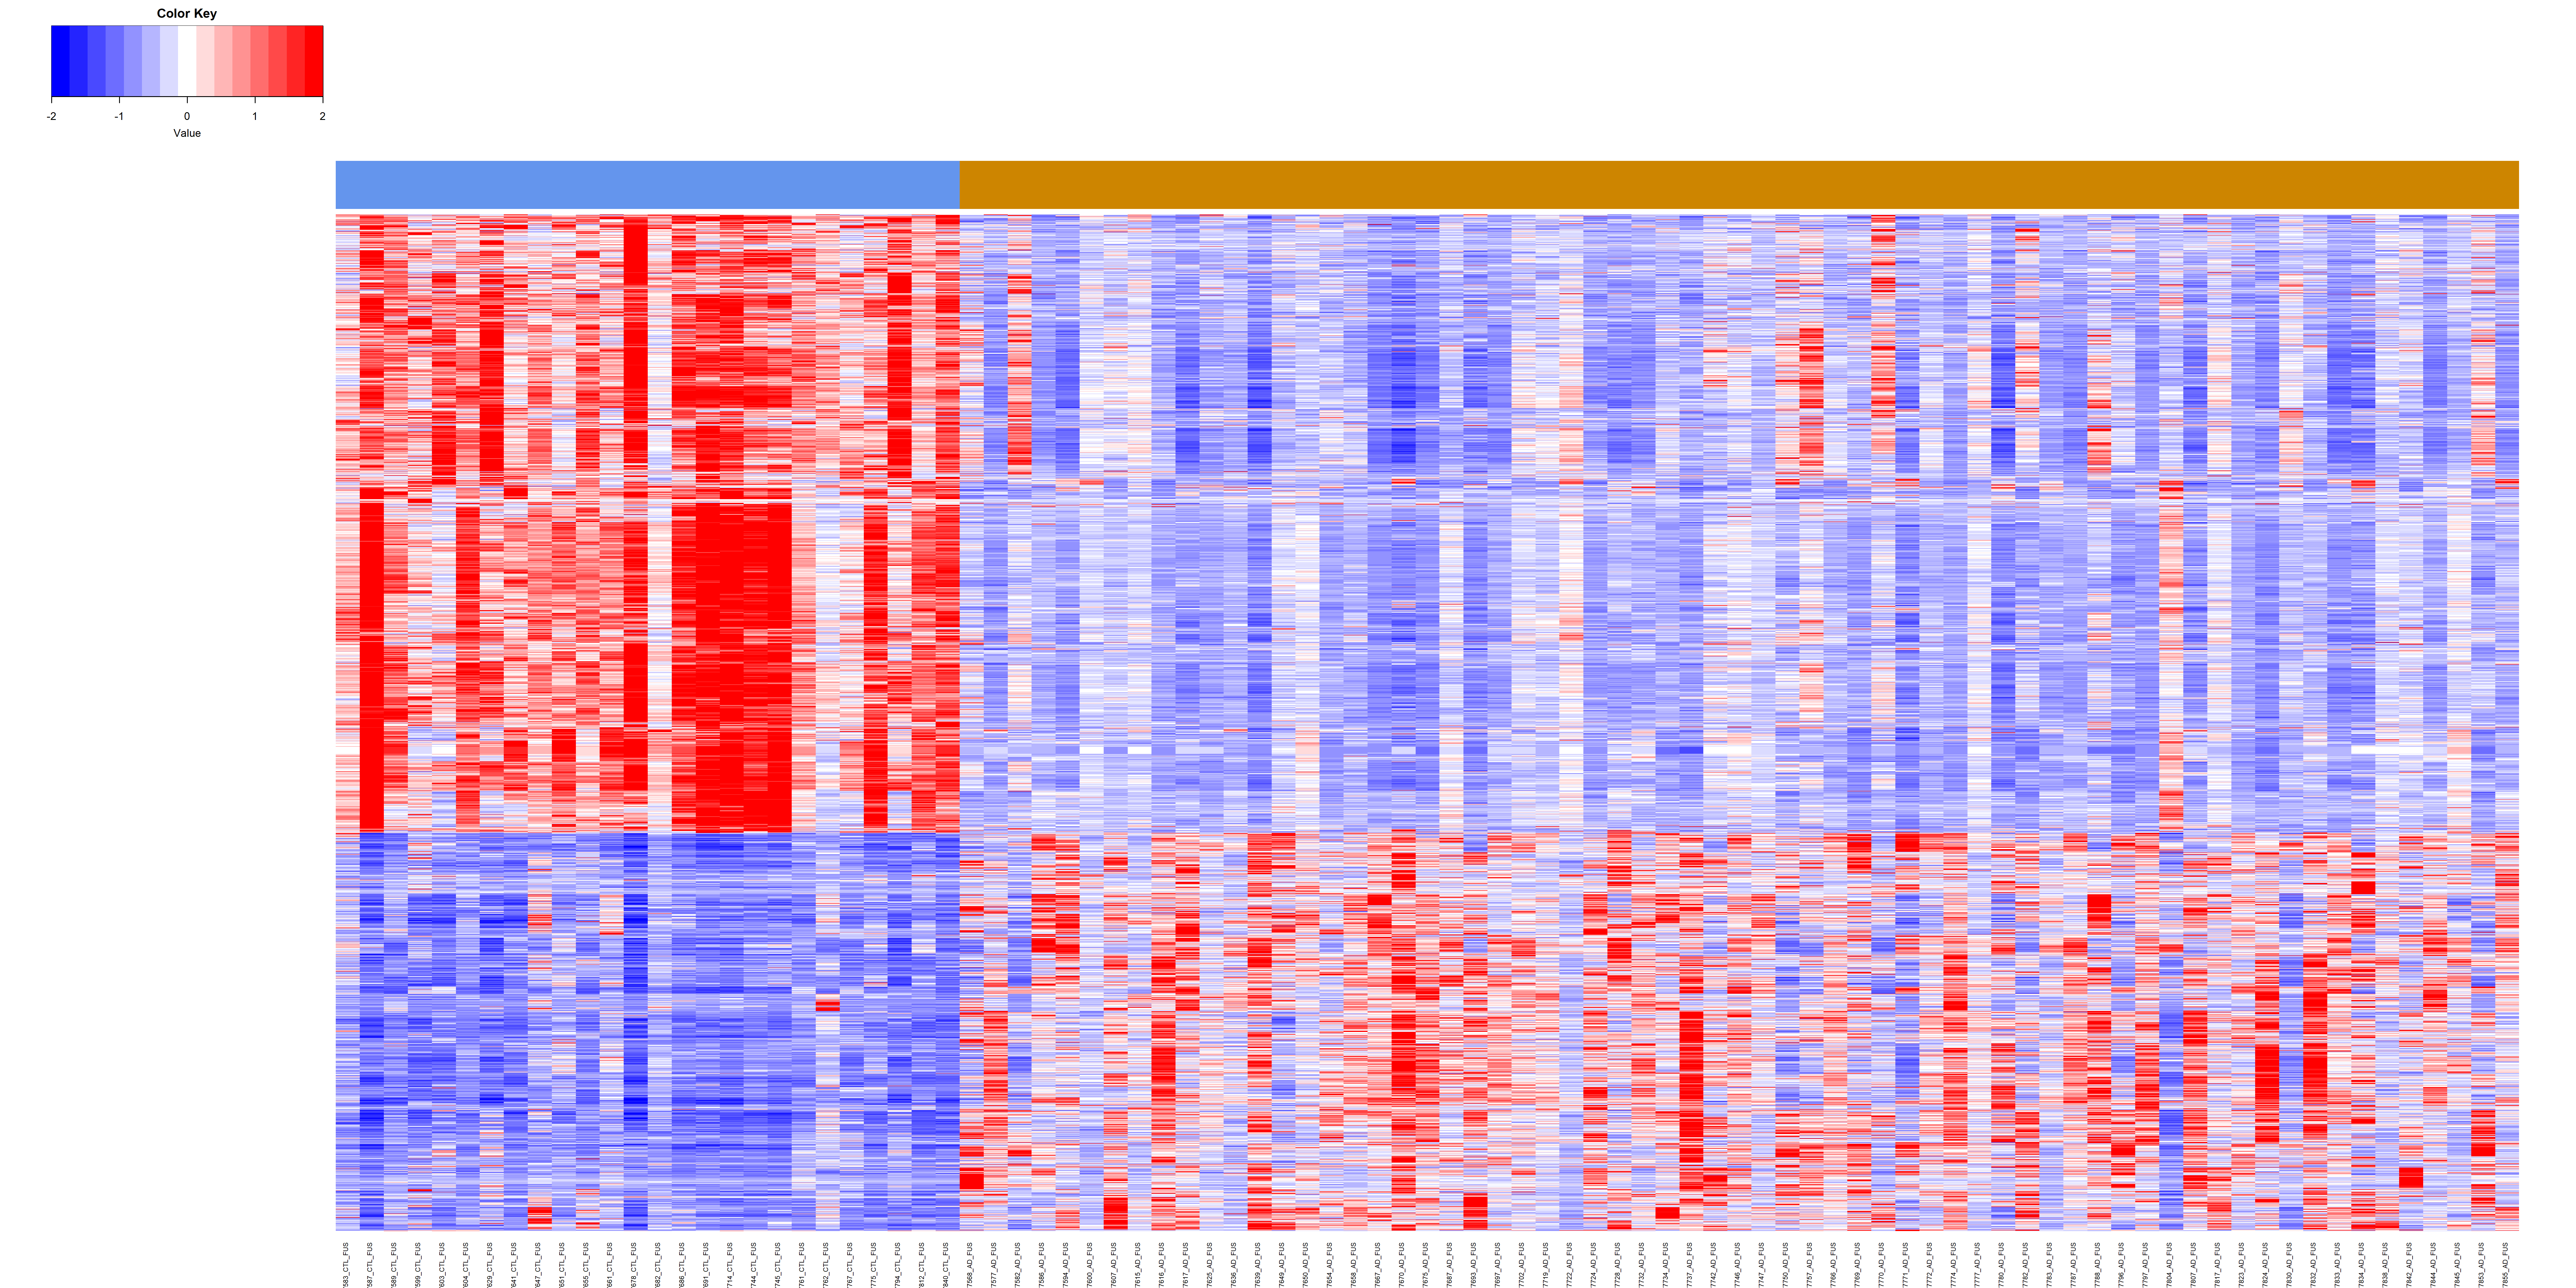
\includegraphics[width = 11cm]{Figures/DE heatmap/CTLvsAD-FUS-f_all.png}}
\caption{Heatmap of Fus-AD-f dataset for all the differentially expressed genes.}
\label{DE-fus-ad-f}
\footnotesize $|$LFC$| >$ 1; AD is the contrast reference. Blue bar: control samples; golden bar: AD samples.
\end{figure}

\begin{figure}[!ht]
    \centerline{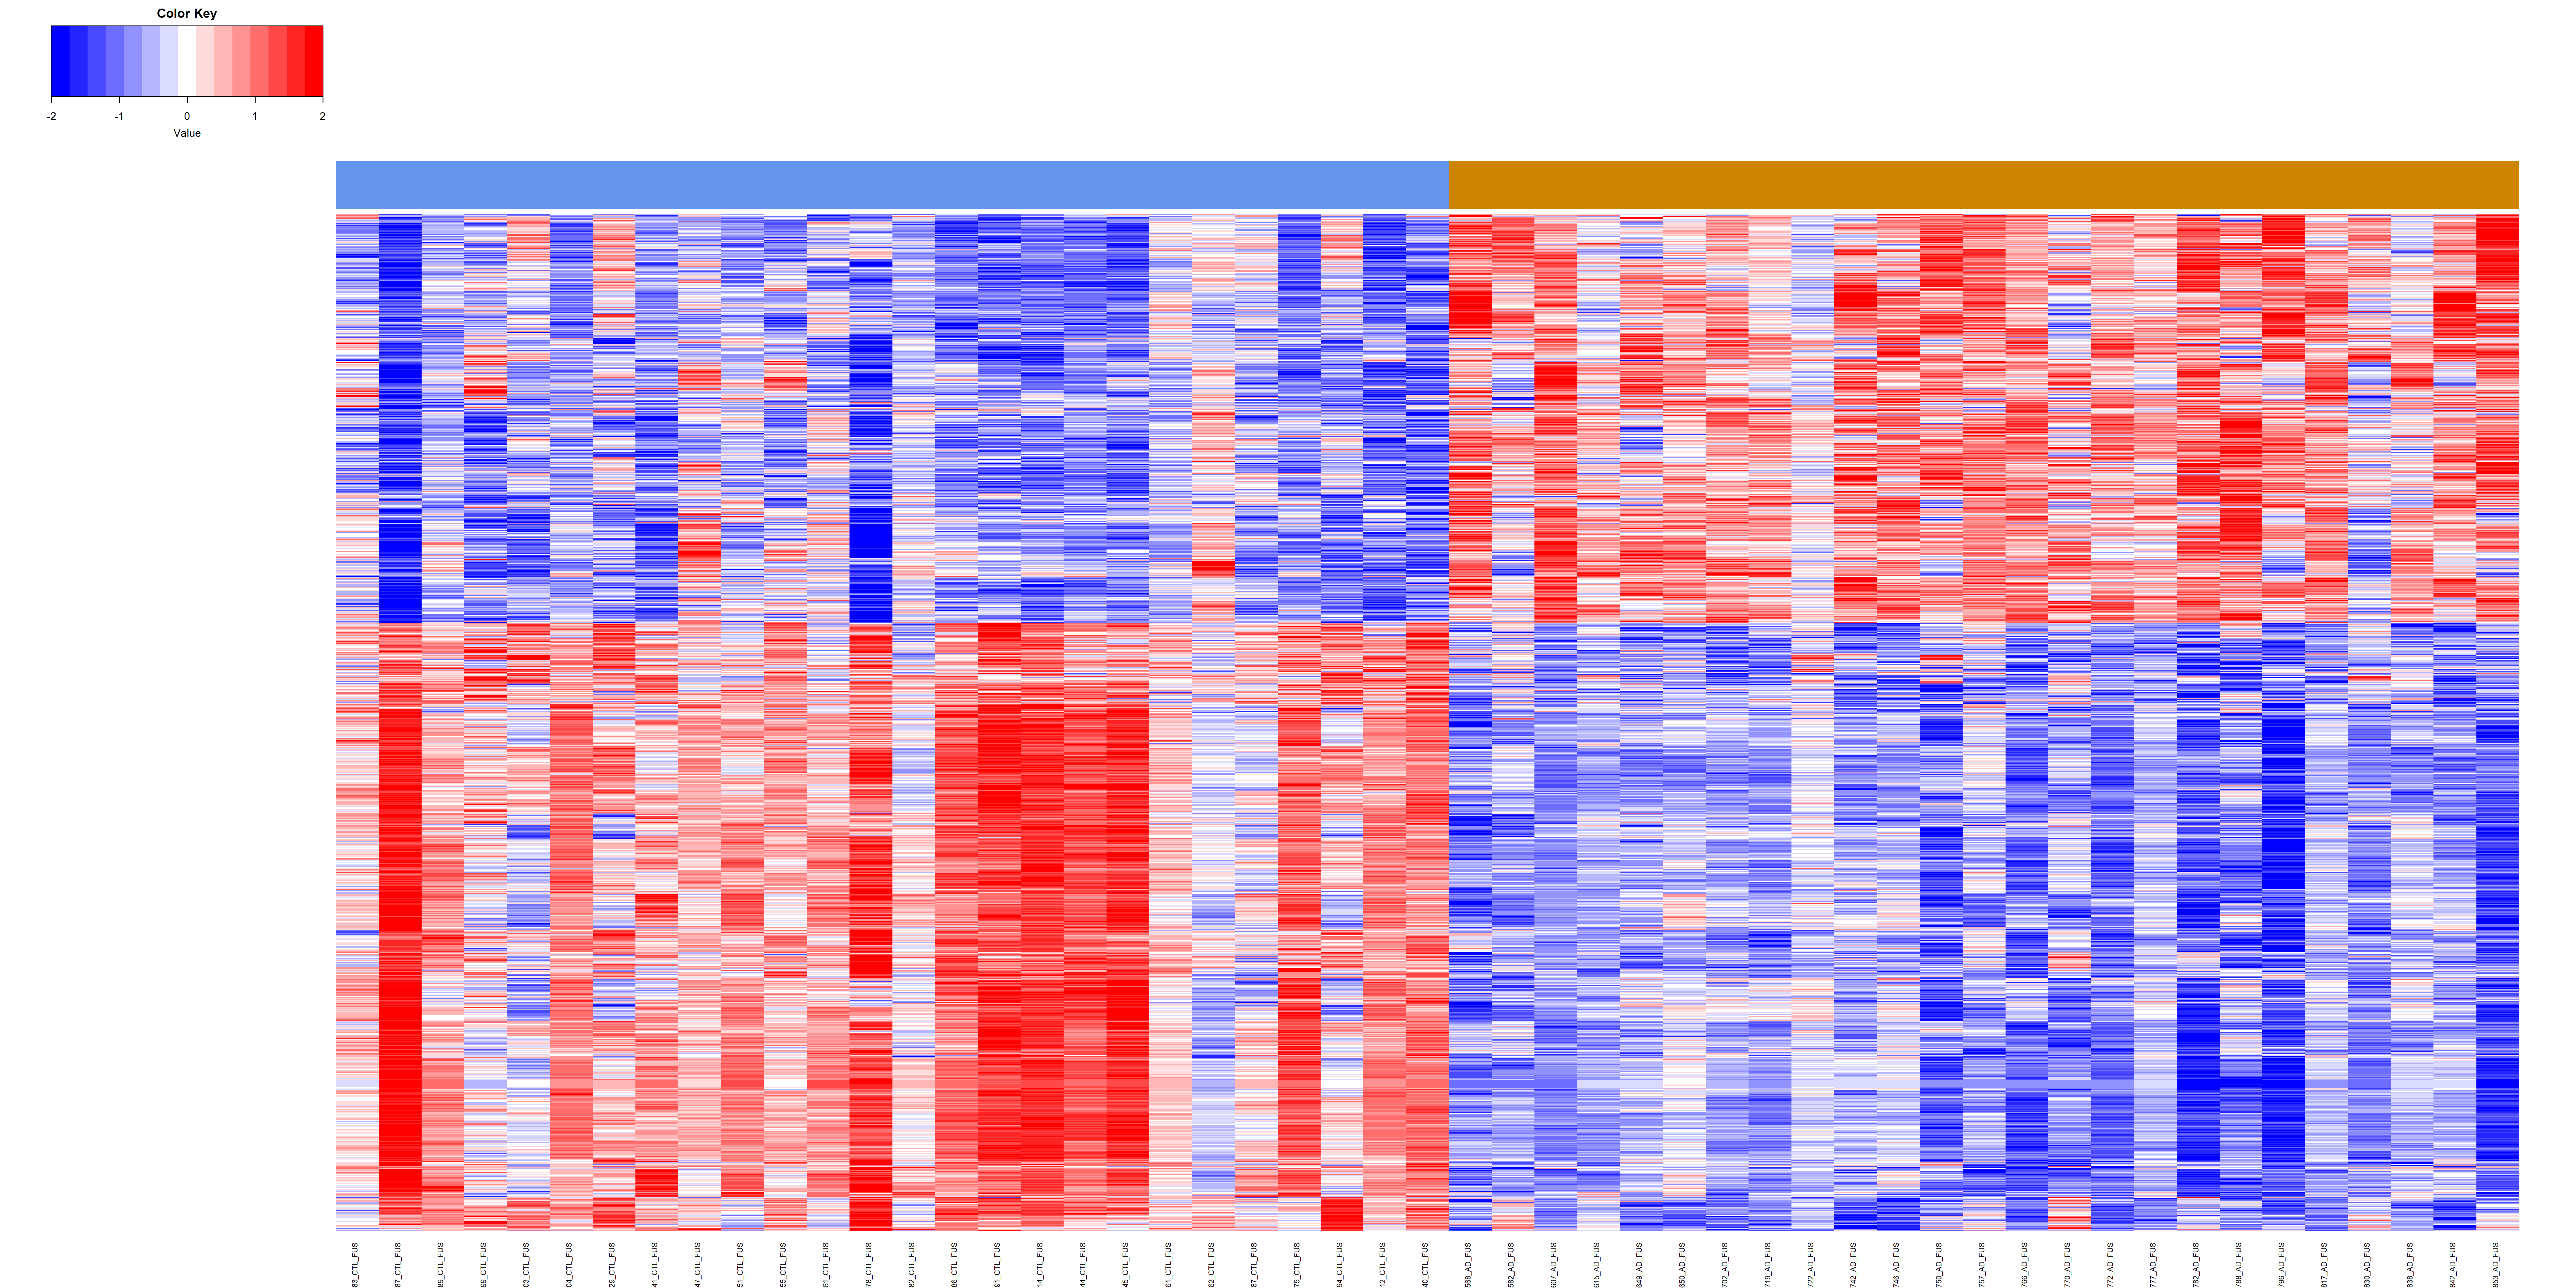
\includegraphics[width = 11cm]{Figures/DE heatmap/CTLvs1_AD-FUS-f_all.png}}
\caption{Heatmap of Fus-AD-f dataset for all the differentially expressed genes between control and subtype 1.}
\footnotesize $|$LFC$| >$ 1.5; case is the contrast reference. Blue bar: control samples; golden bar: S1 samples.
\end{figure}

\begin{figure}[!ht]
    \centerline{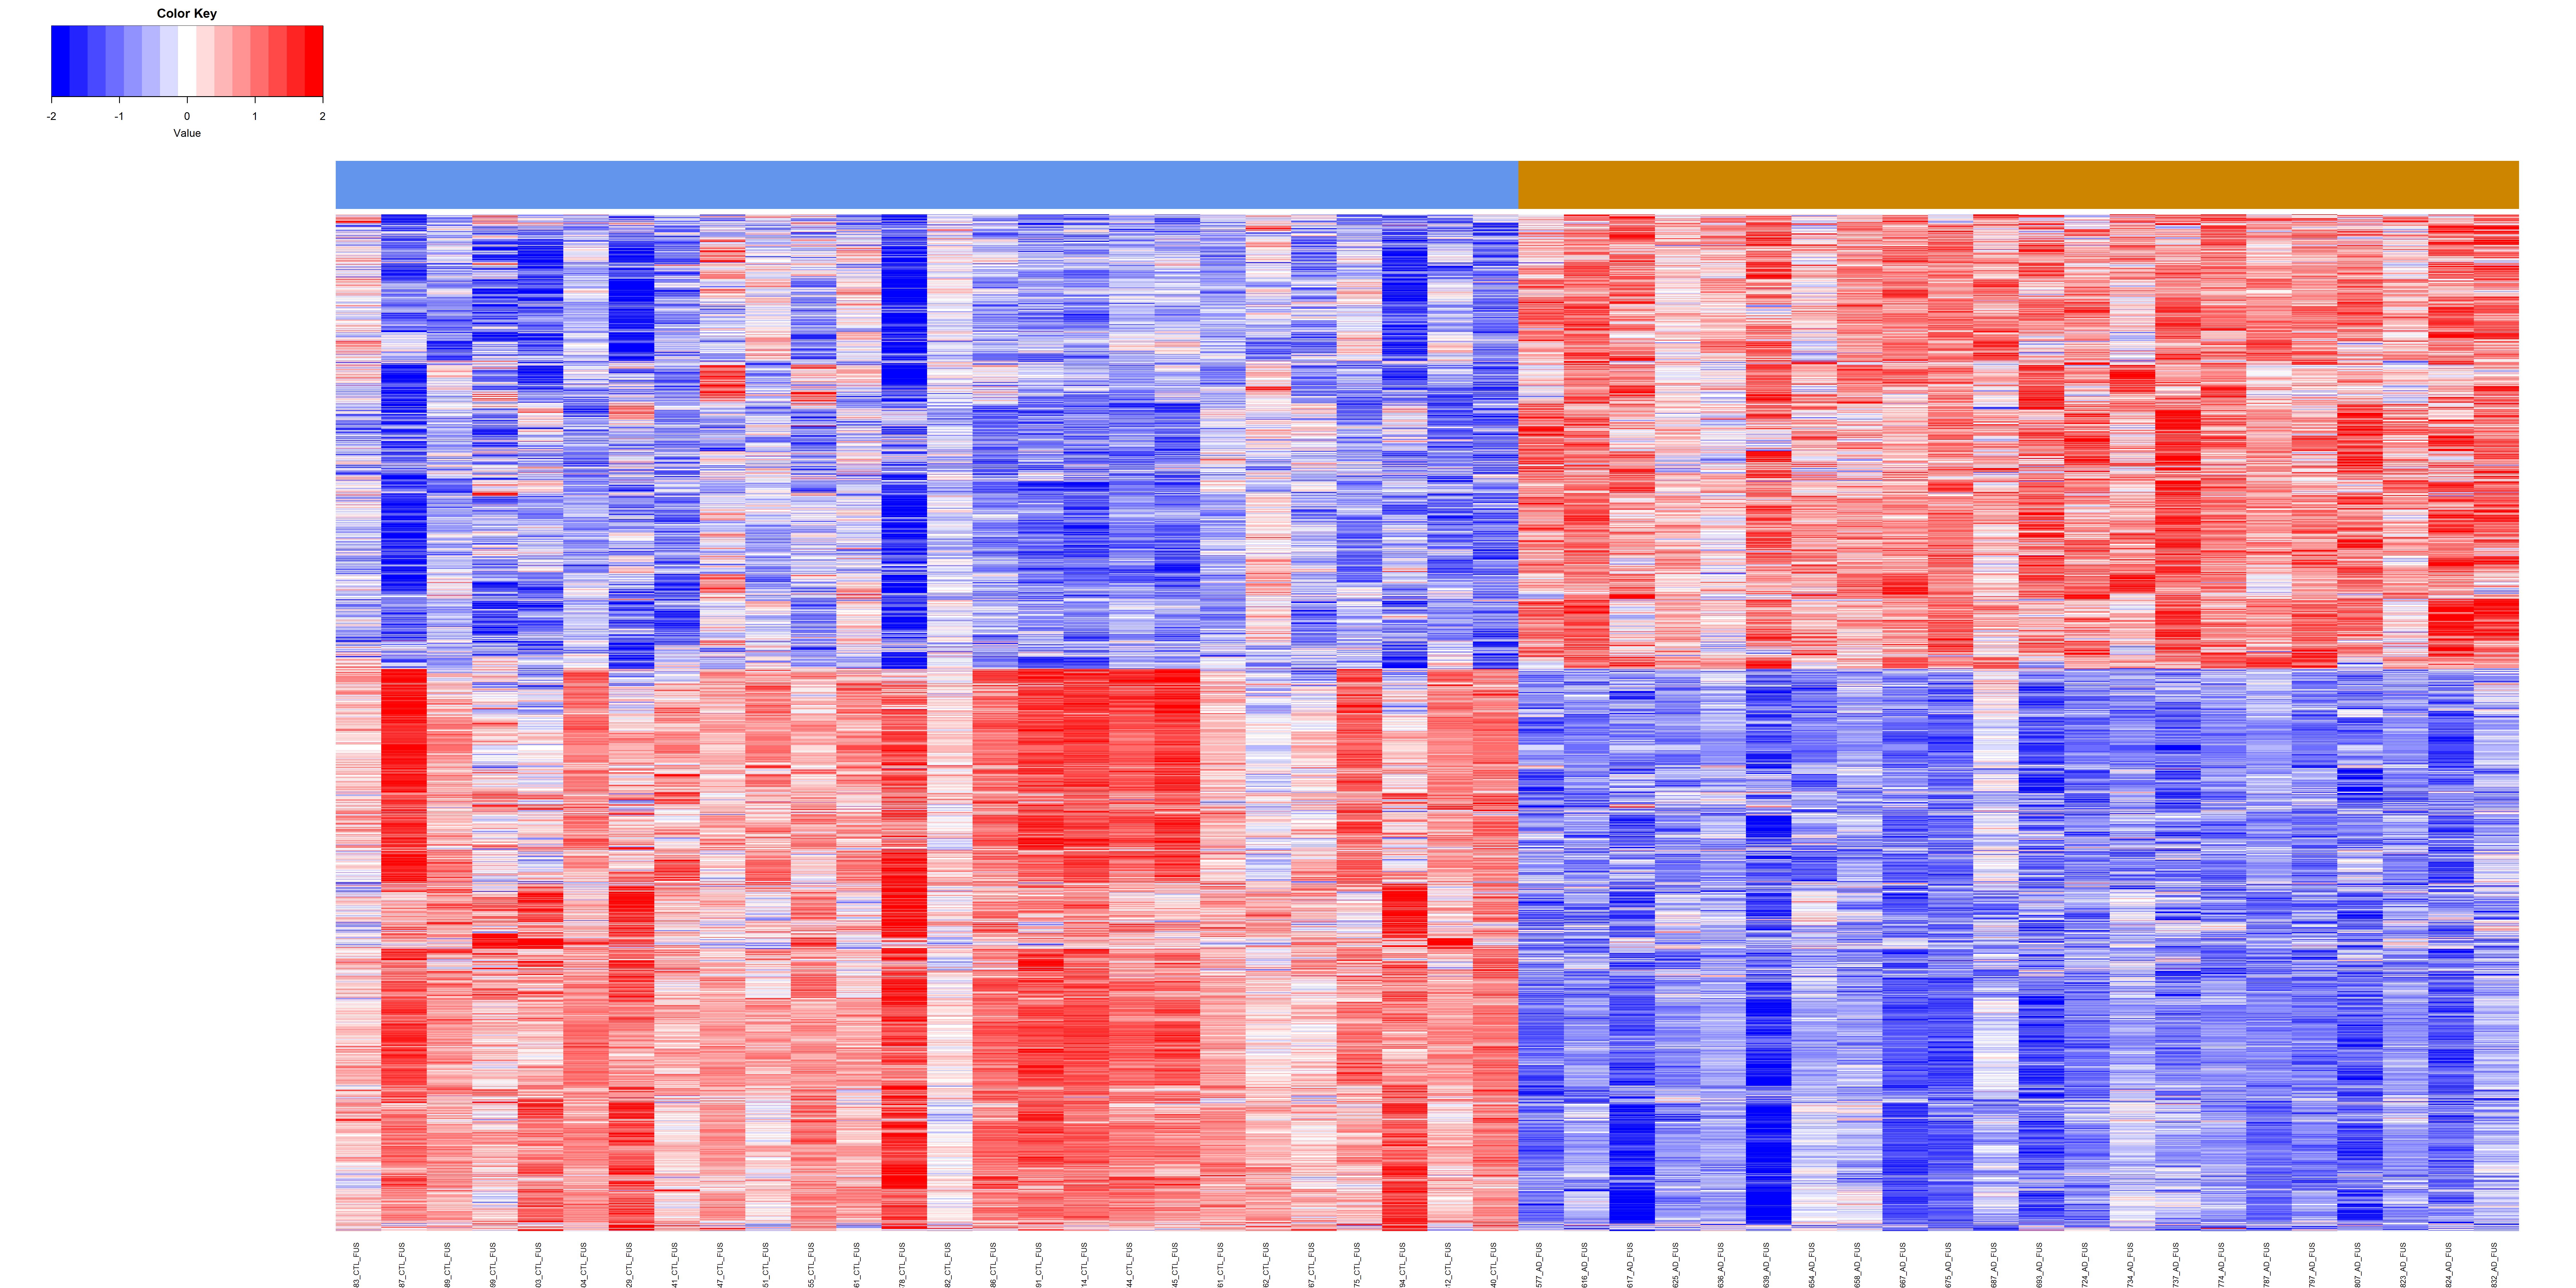
\includegraphics[width = 11cm]{Figures/DE heatmap/CTLvs2_AD-FUS-f_all.png}}
\caption{Heatmap of Fus-AD-f dataset for all the differentially expressed genes between control and subtype 2.}
\footnotesize $|$LFC$| >$ 1.5; case is the contrast reference. Blue bar: control samples; golden bar: S2 samples.
\end{figure}

\begin{figure}[!ht]
    \centerline{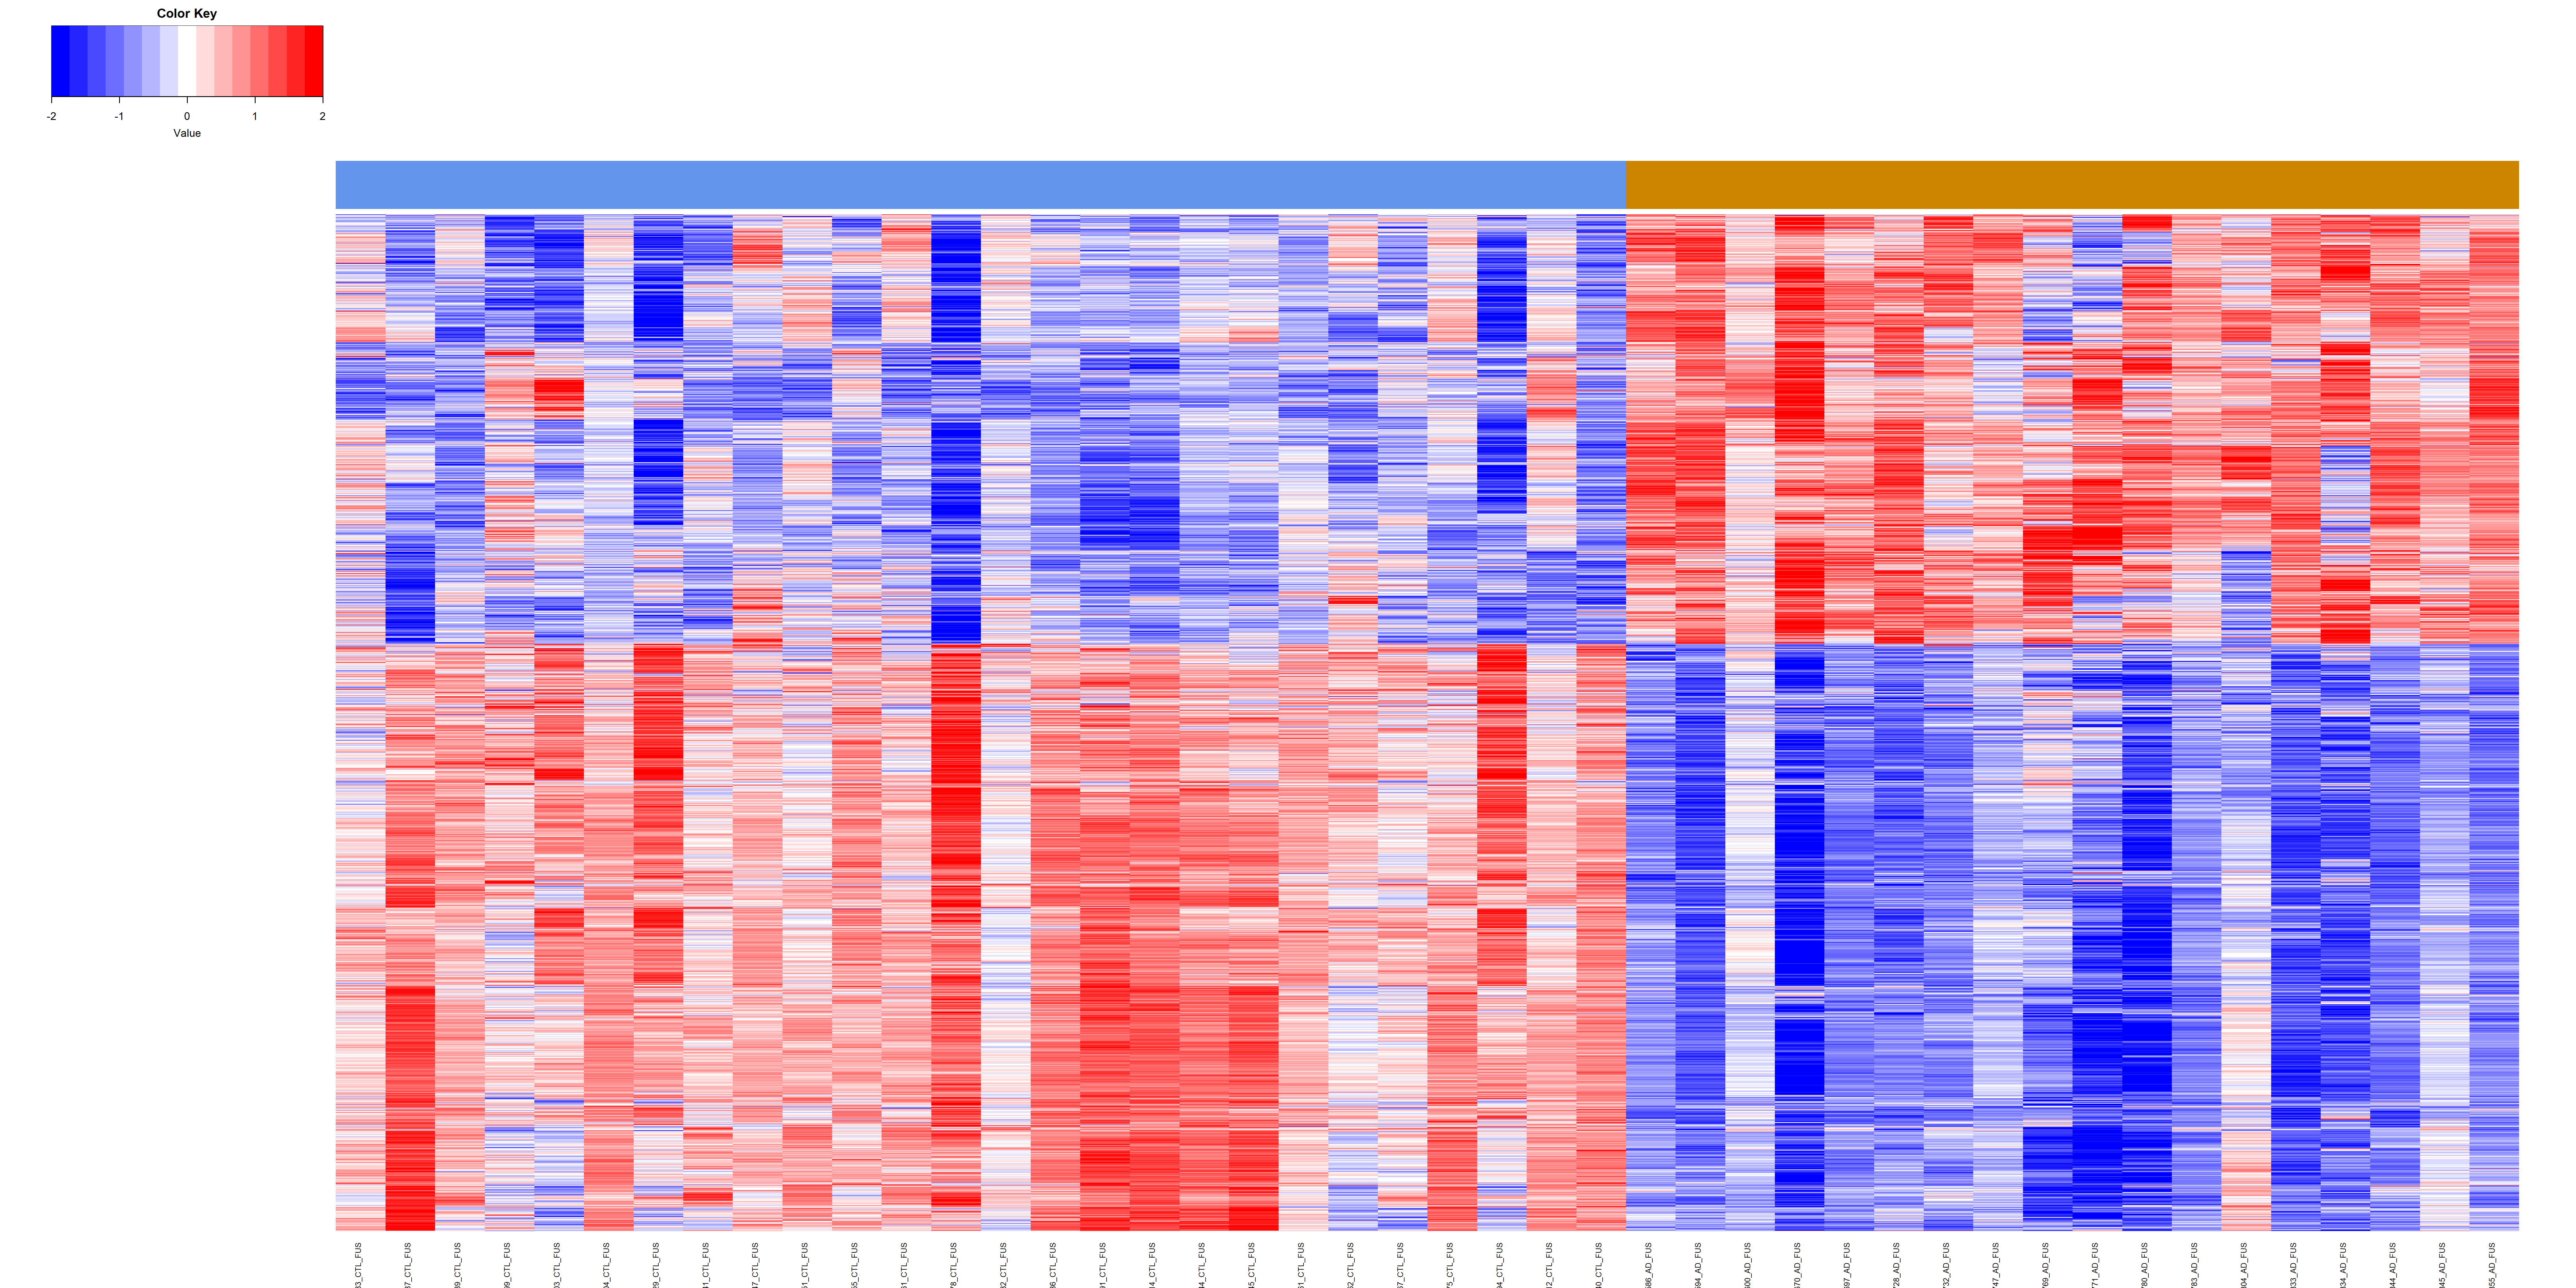
\includegraphics[width = 11cm]{Figures/DE heatmap/CTLvs3_AD-FUS-f_all.png}}
\caption{Heatmap of Fus-AD-f dataset for all the differentially expressed genes between control and subtype 3.}
\footnotesize $|$LFC$| >$ 1.5; case is the contrast reference. Blue bar: control samples; golden bar: S3 samples.
\end{figure}

%\section{Heatmaps for Fus-AD-m comparisons}

\begin{figure}[!ht]
    \centerline{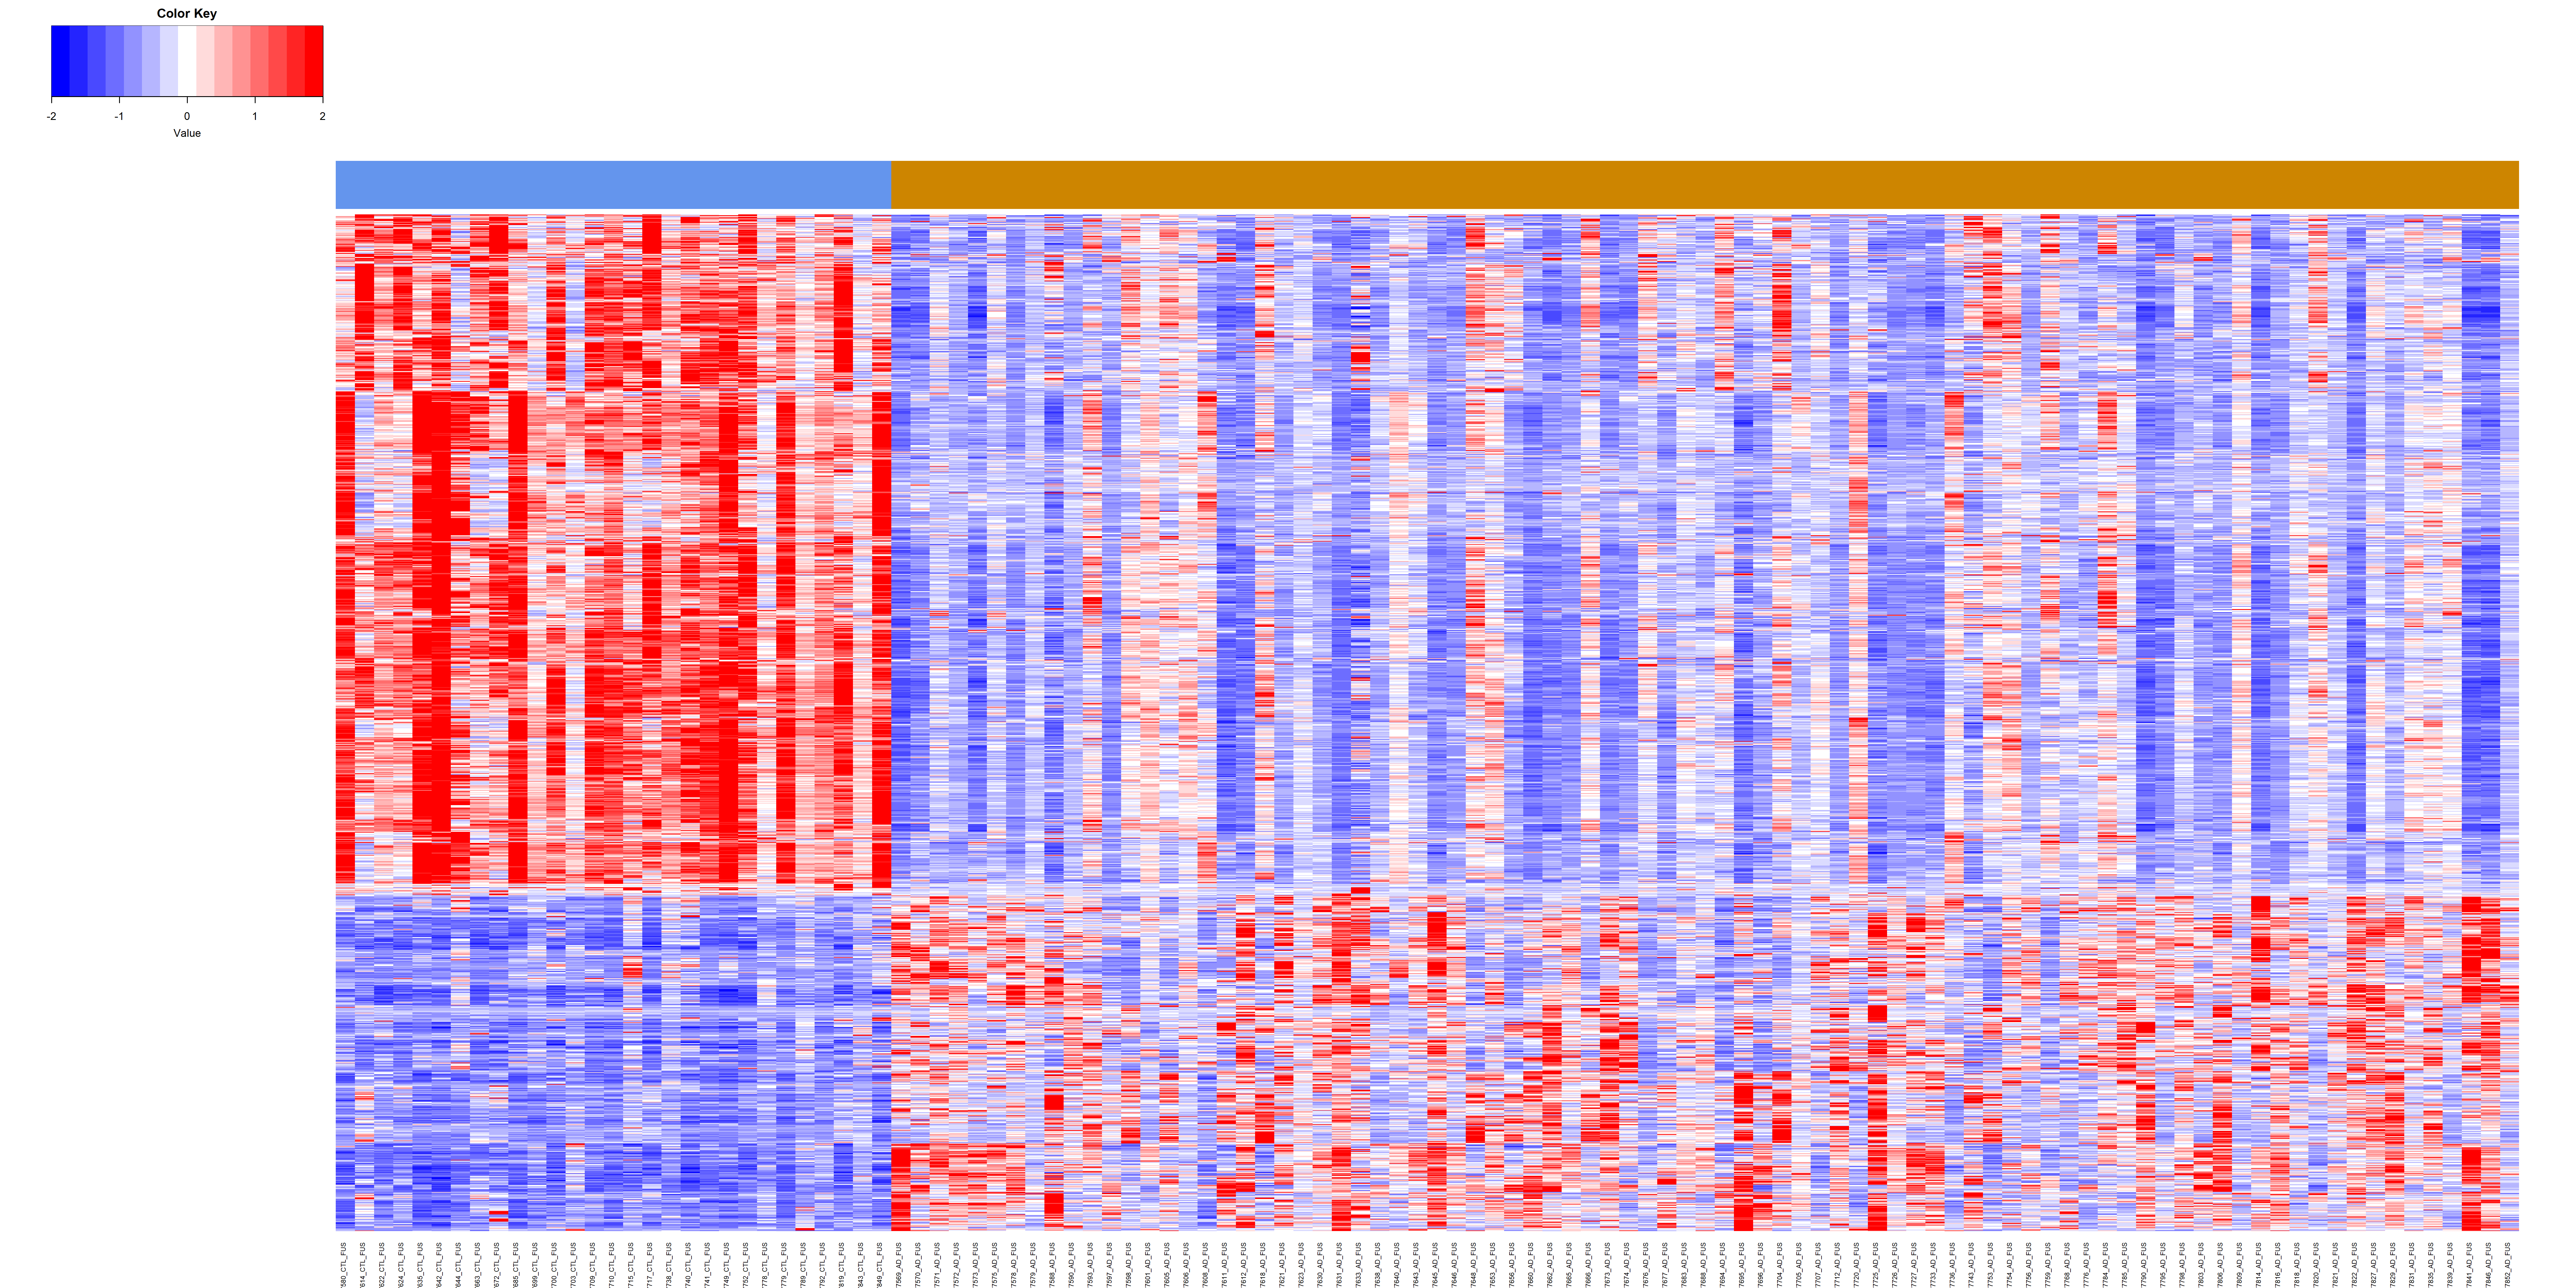
\includegraphics[width = 11cm]{Figures/DE heatmap/CTLvsAD-FUS-m_all.png}}
\caption{Heatmap of Fus-AD-m dataset for all the differentially expressed genes.}
\label{DE-fus-ad-m}
\footnotesize $|$LFC$| >$ 1; AD is the contrast reference. Blue bar: control samples; golden bar: AD samples.
\end{figure}

\begin{figure}[!ht]
    \centerline{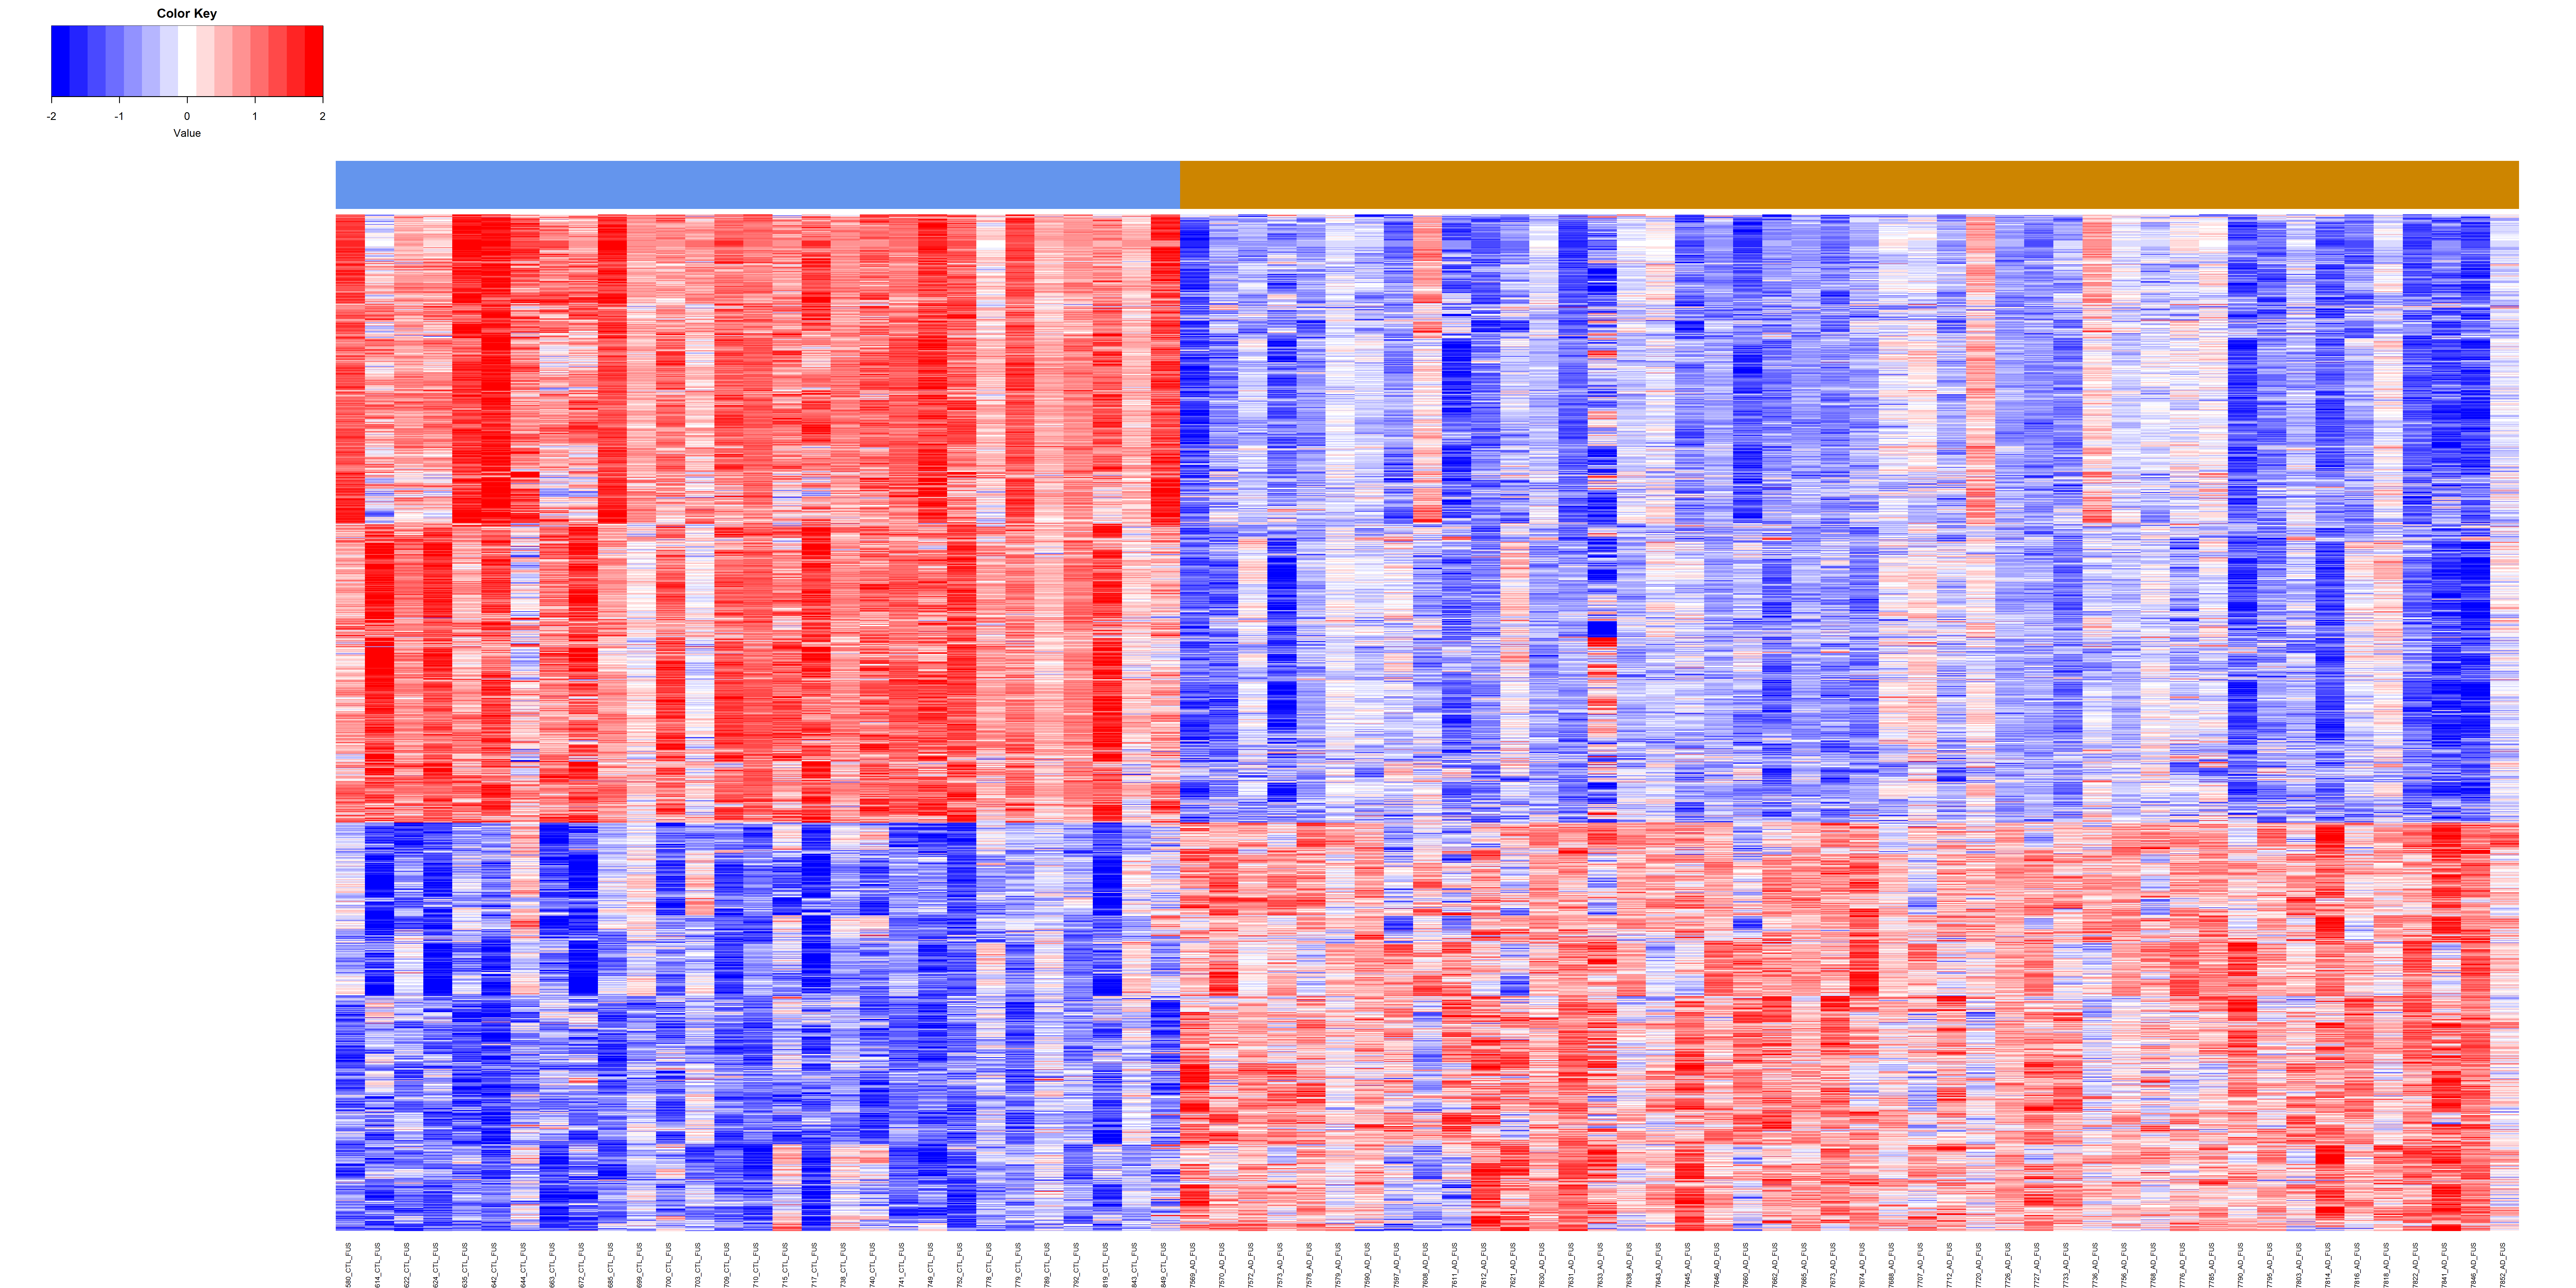
\includegraphics[width = 11cm]{Figures/DE heatmap/CTLvs1_AD-FUS-m_all.png}}
\caption{Heatmap of Fus-AD-m dataset for all the differentially expressed genes between control and subtype 1.}
\footnotesize $|$LFC$| >$ 1.5; case is the contrast reference. Blue bar: control samples; golden bar: S1 samples.
\end{figure}

\begin{figure}[!ht]
    \centerline{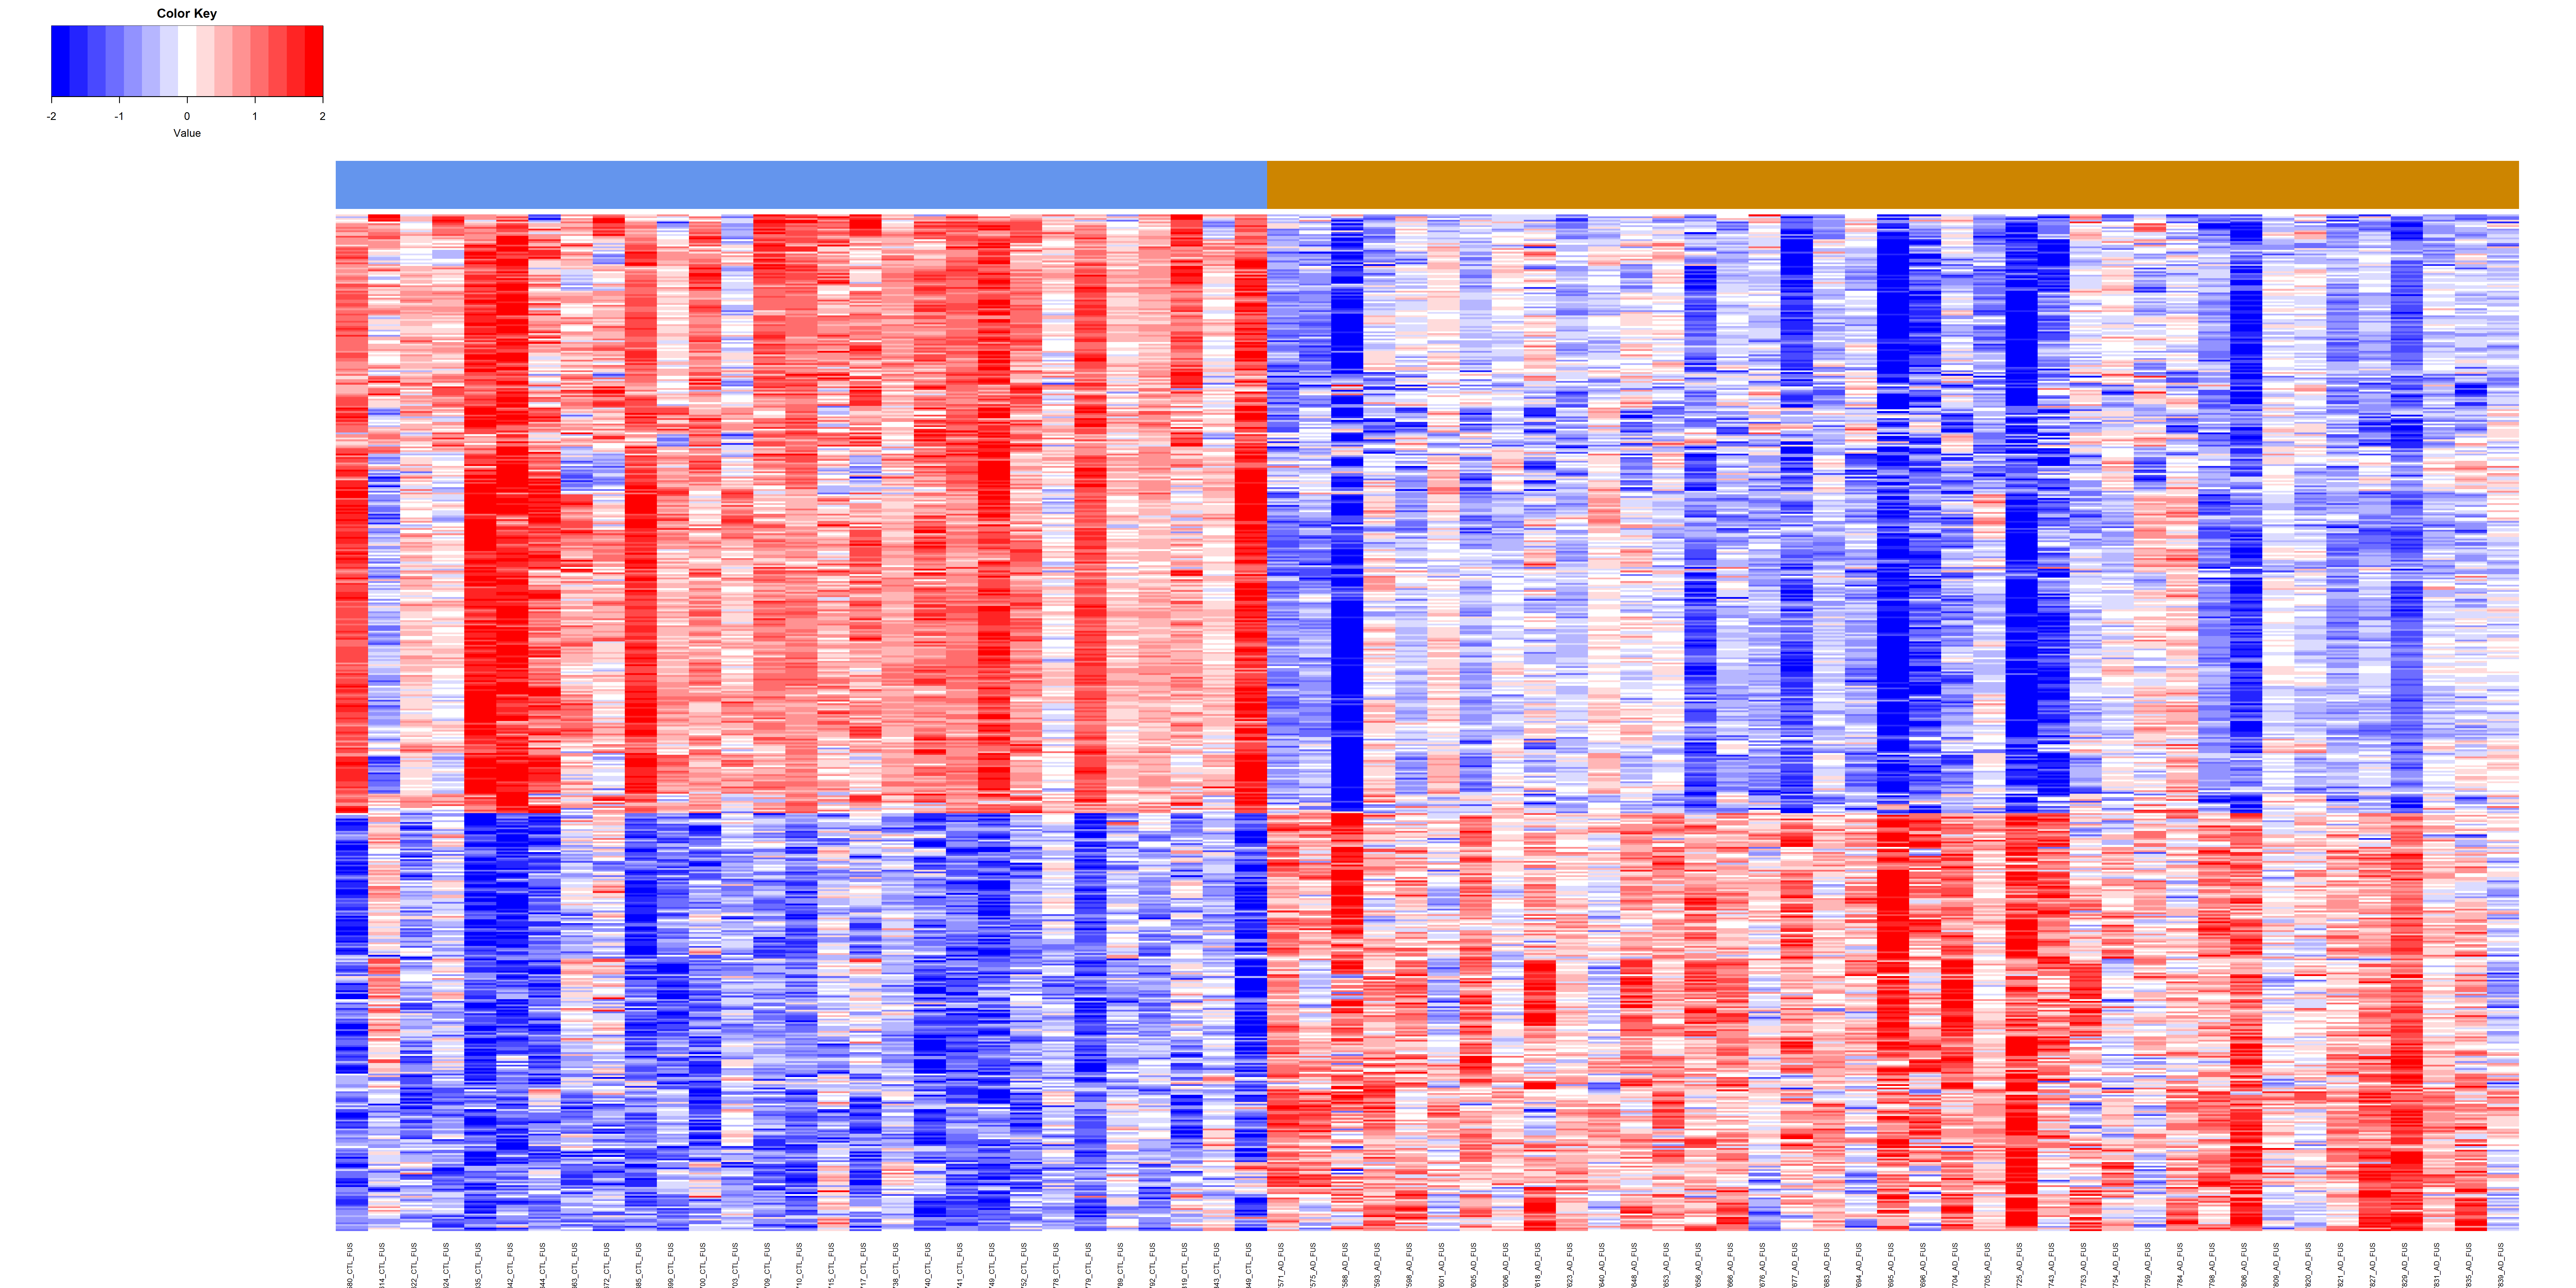
\includegraphics[width = 11cm]{Figures/DE heatmap/CTLvs2_AD-FUS-m_all.png}}
\caption{Heatmap of Fus-AD-m dataset for all the differentially expressed genes between control and subtype 2.}
\footnotesize $|$LFC$| >$ 1.5; case is the contrast reference. Blue bar: control samples; golden bar: S2 samples.
\end{figure}